%
% Template Laporan Skripsi/Thesis Universitas Indonesia
%
% @author  Ichlasul Affan, Azhar Kurnia
% @version 2.1.2
%
% Dokumen ini dibuat berdasarkan standar IEEE dalam membuat class untuk
% LaTeX dan konfigurasi LaTeX yang digunakan Fahrurrozi Rahman ketika
% membuat laporan skripsi, yang kemudian diadaptasi oleh Andreas Febrian dan
% Lia Sadita untuk template skripsi tahun 2010.
% Konfigurasi template sebelumnya telah disesuaikan dengan
% aturan penulisan thesis yang dikeluarkan UI pada tahun 2017.
%

%
% Tipe dokumen adalah report dengan satu kolom.
%
\documentclass[12pt, a4paper, onecolumn, twoside, final]{report}
\raggedbottom

% Load konfigurasi LaTeX untuk tipe laporan thesis
\usepackage{_internals/uithesis}
%

% Load konfigurasi khusus untuk laporan yang sedang dibuat
%-----------------------------------------------------------------------------%
% Informasi Mengenai Dokumen
%-----------------------------------------------------------------------------%
%
% Judul laporan.
% \def\judul{Analisis pengaruh Load Balancing terhadap Performa Aplikasi Web Service dalam Multi-Region Kubernetes Cluster}
\def\judul{Analisis Performa Aplikasi Web Service dalam Multi-Region Geo-Distributed Kubernetes Cluster}
%
% Tulis kembali judul laporan, kali ini akan diubah menjadi huruf kapital
% \Var{\Judul}{Analisis pengaruh Load Balancing terhadap Performa Aplikasi Web Service dalam Multi-Region Kubernetes Cluster}
\Var{\Judul}{Analisis Performa Aplikasi Web Service dalam Multi-Region Geo-Distributed Kubernetes Cluster}
%
% Tulis kembali judul laporan namun dengan bahasa Ingris
\def\judulInggris{Web Application Performance Analysis of Multi-Region Geo-Distributed Kubernetes Clusters}

\Var{\JudulInggris}{Web Application Performance Analysis of Multi-Region Geo-Distributed Kubernetes Clusters}

%
% Tipe laporan, dapat berisi: Laporan Kerja Praktik, Skripsi, Tugas Akhir, Thesis, atau Disertasi
\def\type{Skripsi}
%
% Jenjang studi, dapat berisi: Diploma, Sarjana, Magister, atau Doktor
\def\jenjang{Sarjana}
%
% Tulis kembali tipe laporan, kali ini akan diubah menjadi huruf kapital
\Var{\Type}{Skripsi}
%
% Tulis nama penulis
\def\penulis{Jonathan Nicholas}
%
% Tulis kembali nama penulis, kali ini akan diubah menjadi huruf kapital
\Var{\Penulis}{Jonathan Nicholas}
%
% Tulis NPM penulis
\def\npm{1906293133}
%
% Tuliskan Fakultas dimana penulis berada
\Var{\Fakultas}{Ilmu Komputer}
\def\fakultas{Ilmu Komputer}
%
% Tuliskan Program Studi yang diambil penulis
\Var{\Program}{Ilmu Komputer}
\def\program{Ilmu Komputer}
% Program Studi dalam bahasa inggris
\def\studyProgram{Computer Science}
%
% Tuliskan tahun publikasi laporan
\Var{\bulanTahun}{Mei 2023}
%
% Tuliskan gelar yang akan diperoleh dengan menyerahkan laporan ini
\def\gelar{Gelar Jurusan Anda}
%
% Tuliskan tanggal pengesahan laporan, waktu dimana laporan diserahkan ke
% penguji/sekretariat
\def\tanggalSiapSidang{09 Juni 2023}
%
% Tuliskan tanggal keputusan sidang dikeluarkan dan penulis dinyatakan
% lulus/tidak lulus
\def\tanggalLulus{21 Juni 2023}
%
% Tuliskan pembimbing
\def\pembimbingSatu{Muhammad Hafizhuddin Hilman, S.Kom., M.Kom.}
% S1 s.d. S3: Kosongkan jika tidak ada pembimbing kedua
\def\pembimbingDua{}
% S2 & S3: Kosongkan jika tidak ada pembimbing ketiga
\def\pembimbingTiga{}
%
% Tuliskan penguji
\def\pengujiSatu{Amril Syalim, S.Kom., M.Eng., Ph.D.}
\def\pengujiDua{Penguji Kedua Anda}
% Kosongkan jika tidak ada penguji ketiga (umumnya penguji ketiga hanya ada untuk S2)
\def\pengujiTiga{Made Harta Dwijaksara, S.T., M.Sc., Ph.D.}
% Kosongkan jika tidak ada penguji keempat, kelima, atau keenam (umumnya penguji > 3 hanya ada untuk S3)
\def\pengujiEmpat{}
\def\pengujiLima{}
\def\pengujiEnam{}

%-----------------------------------------------------------------------------%
% Judul Setiap Bab
%-----------------------------------------------------------------------------%
%
% Berikut ada judul-judul setiap bab.
% Silahkan diubah sesuai dengan kebutuhan.
%
\Var{\kataPengantar}{Acknowledgement}
\Var{\babSatu}{Introduction}
\Var{\babDua}{Literature Review}
\Var{\babTiga}{Methodology}
\Var{\babEmpat}{Design and Implementation}
\Var{\babLima}{Results and Analysis}
\Var{\kesimpulan}{Conclusion}

% Daftar pemenggalan suku kata dan istilah dalam LaTeX
% %
% Hyphenation untuk Indonesia
%
% @author  Andreas Febrian
% @version 2.1.2
% @edit by Ichlasul Affan, Muhammad Aulia Adil Murtito
%
% Tambahkan cara pemenggalan kata-kata yang salah dipenggal secara otomatis
% oleh LaTeX. Jika kata tersebut dapat dipenggal dengan benar, maka tidak
% perlu ditambahkan dalam berkas ini. Tanda pemenggalan kata menggunakan
% tanda '-'; contoh:
% menarik
%   --> pemenggalan: me-na-rik
%


% Silakan ganti ke bahasa Inggris (\selectlanguage{english}) jika Anda merasa terlalu banyak kata bahasa Inggris yang pemenggalannya tidak benar.
%\selectlanguage{english}


\hyphenation{
    % alphabhet A
    a-na-li-sa a-tur a-tur-an
    a-pli-ka-si
    % alphabhet B
    bab ba-ngun-an
    be-be-ra-pa
    ber-ge-rak
    ber-ke-lan-jut-an
    ber-o-per-ra-si
    ber-pe-nga-ruh
    % alphabhet C
    ca-ri Com-po-nent-UML
    % alphabhet D
    di-da-pat-kan di-sim-pan di-pim-pin di-tam-bah-kan di-tem-pat-kan de-ngan da-e-rah di-ba-ngun di-gu-na-kan da-pat di-nya-ta-kan
    di-se-mat-kan di-sim-bol-kan di-pi-lih di-li-hat de-fi-ni-si di-de-fi-ni-si-kan di-mo-del-kan di-mi-li-ki di-re-a-li-sa-si-kan di-su-sun
    % alphabhet E
    eks-pli-sit e-ner-gi en-gi-neer en-gi-neer-ing eks-klu-sif ele-men
    % alphabhet F
    fa-si-li-tas
    % alphabhet G
    ga-bung-an ge-rak ge-ne-ral ge-ne-ra-li-sa-si
    % alphabhet H
    ha-lang-an
    % alphabhet I
    in-fra-struk-tur i-ni-si-a-si
    % alphabhet J
    % alphabhet K
    ke-hi-lang-an
    ke-ter-hu-bung-an
    ku-ning
    kua-li-tas ka-me-ra ke-mung-kin-an ke-se-pa-ham-an
    % alphabhet L
    ling-kung-an
    % alphabhet M
    ma-na-je-men me-neng-ah meng-a-da-kan me-mo-ni-tor
    me-mer-lu-kan me-mo-del-kan men-de-fi-ni-si-kan meng-ak-ses me-ne-mu-kan
    meng-a-tas-i me-mo-di-fi-ka-si me-mung-kin-kan me-nge-na-i me-ngi-rim-kan meng-i-zin-kan
    meng-u-bah meng-a-dap-ta-si me-nya-ta-kan me-nyim-pan me-res-trik-si mi-cro-ser-vi-ce mi-cro-ser-vi-ces mo-di-fi-ka-si mo-dul mo-dule
    meng-a-tur meng-a-rah-kan mi-lik meng-gu-na-kan me-ne-ri-ma me-nga-la-mi
    % alphabhet N
    nya-ta non-eks-klu-sif
    % alphabhet O
    o-pe-ra-si or-ga-ni-sa-si
    % alphabhet P
	pe-nye-rap-an
	pe-ngon-trol
    pe-mo-del-an
    pe-ran  pe-ran-an-nya
    pem-ba-ngun-an pre-si-den pe-me-rin-tah pe-mi-li-han prio-ri-tas peng-am-bil-an
    peng-ga-bung-an pe-nga-was-an pe-ngem-bang-an
    pe-nga-ruh pe-nge-lo-la pa-ra-lel-is-me per-hi-tung-an per-ma-sa-lah-an
    pen-ca-ri-an pen-ce-ta-kan peng-struk-tur-an pen-ting pen-ting-nya pe-ngu-ku-ran
    pre-sen-ta-si
    % alphabhet Q
    % alphabhet R
    ran-cang-an re-fe-ren-si re-pre-sen-ta-si
    % alphabhet S
    sub-bab si-mu-la-si sa-ngat ska-la-bi-li-tas
    stan-dar-di-sa-si
    % alphabhet T
    te-ngah
    ter-da-pat
    trans-for-ma-si
    % alphabhet U
    % alphabhet V
    va-li-da-si va-ri-an va-ri-a-si va-ri-a-bi-li-tas ve-ri-fi-ka-si
    % alphabhet W
    % alphabhet X
    % alphabhet Y
    % alphabhet Z
    % special
}

% Daftar istilah yang mungkin perlu ditandai
%
% @author  Andreas Febrian
% @version 1.00
%
% Mendaftar seluruh istilah yang mungkin akan perlu dijadikan
% italic atau bold pada setiap kemunculannya dalam dokumen.
%

\var{\license}{\f{Creative Common License 1.0 Generic}}
\var{\bslash}{$\setminus$}


% Awal bagian penulisan laporan
\begin{document}
%
% Sampul Laporan
%
% Sampul Laporan

%
% @author  unknown
% @version 1.01
% @edit by Andreas Febrian
%

\begin{titlepage}
    \begin{center}
        \begin{figure}
            \begin{center}
                
\includegraphics[width=2.5cm]{assets/pics/makara_kuning.png}
            \end{center}
        \end{figure}
        \vspace*{0cm}
        \bo{
        	UNIVERSITAS INDONESIA\\
        }

        \vspace*{1.0cm}
        % judul thesis harus dalam 14pt Times New Roman
        \bo{\JudulInggris} \\[1.0cm]

        \vspace*{2.5 cm}
        % harus dalam 14pt Times New Roman
        \bo{\Type}

        \vspace*{3 cm}
        % penulis dan npm
        \bo{\Penulis} \\
        \bo{\npm} \\

        \vspace*{5.0cm}

        % informasi mengenai fakultas dan program studi
        \bo{
        	FAKULTAS \Fakultas\\
        	PROGRAM STUDI \Program \\
        	DEPOK \\
        	\bulanTahun
        }
    \end{center}
\end{titlepage}

\forceclearchapter

%
% Gunakan penomeran romawi
\pagenumbering{roman}
%
% Menghilangkan penebalan pada huruf-huruf table of content
% dari halaman judul hingga daftar lampiran
\disableboldchapterintoc
%
% load halaman judul dalam
\addChapter{HALAMAN JUDUL}
%
% Halaman Judul Laporan
%
% @author  unknown
% @version 1.01
% @edit by Andreas Febrian
%

\begin{titlepage}
    \begin{center}\begin{figure}
            \begin{center}
                
\includegraphics[width=2.5cm]{assets/pics/makara.png}
            \end{center}
        \end{figure}
        \vspace*{0cm}
        \bo{
        	UNIVERSITAS INDONESIA\\
        }

        \vspace*{1.0cm}
        % judul thesis harus dalam 14pt Times New Roman
        \bo{\JudulInggris} \\[1.0cm]

        \vspace*{2.5 cm}
        % harus dalam 14pt Times New Roman
        \bo{\Type} \\
        % keterangan prasyarat
        \bo{Diajukan sebagai salah satu syarat untuk memperoleh gelar \\
        \gelar}\\

        \vspace*{3 cm}
        % penulis dan npm
        \bo{\Penulis} \\
        \bo{\npm} \\

        \vspace*{5.0cm}

        % informasi mengenai fakultas dan program studi
        \bo{
        	FAKULTAS \Fakultas\\
        	PROGRAM STUDI \Program \\
        	DEPOK \\
        	\bulanTahun
        }
    \end{center}
\end{titlepage}

\forceclearchapter

%
% load halaman orisinalitas

% Menghilangkan penomoran
\pagenumbering{gobble}

\strcompare{Laporan Kerja Praktik}{\type}{}
{
	%
% Halaman Orisinalitas
%
% @author  Andreas Febrian
% @version 2.1.2
% @edit by Muhammad Aulia Adil Murtito
%

\chapter*{\uppercase{Halaman Pernyataan Orisinalitas}}
\thispagestyle{empty}
\vspace*{2cm}

% Untuk input gambar tanda tangan, silahkan sesuaikan xshift, yshift, dan width dengan gambar tanda tangan Anda
%\begin{tikzpicture}[remember picture,overlay,shift={(current page.north east)}]
%\node[anchor=north east,xshift=-8.5cm,yshift=-14.2cm]{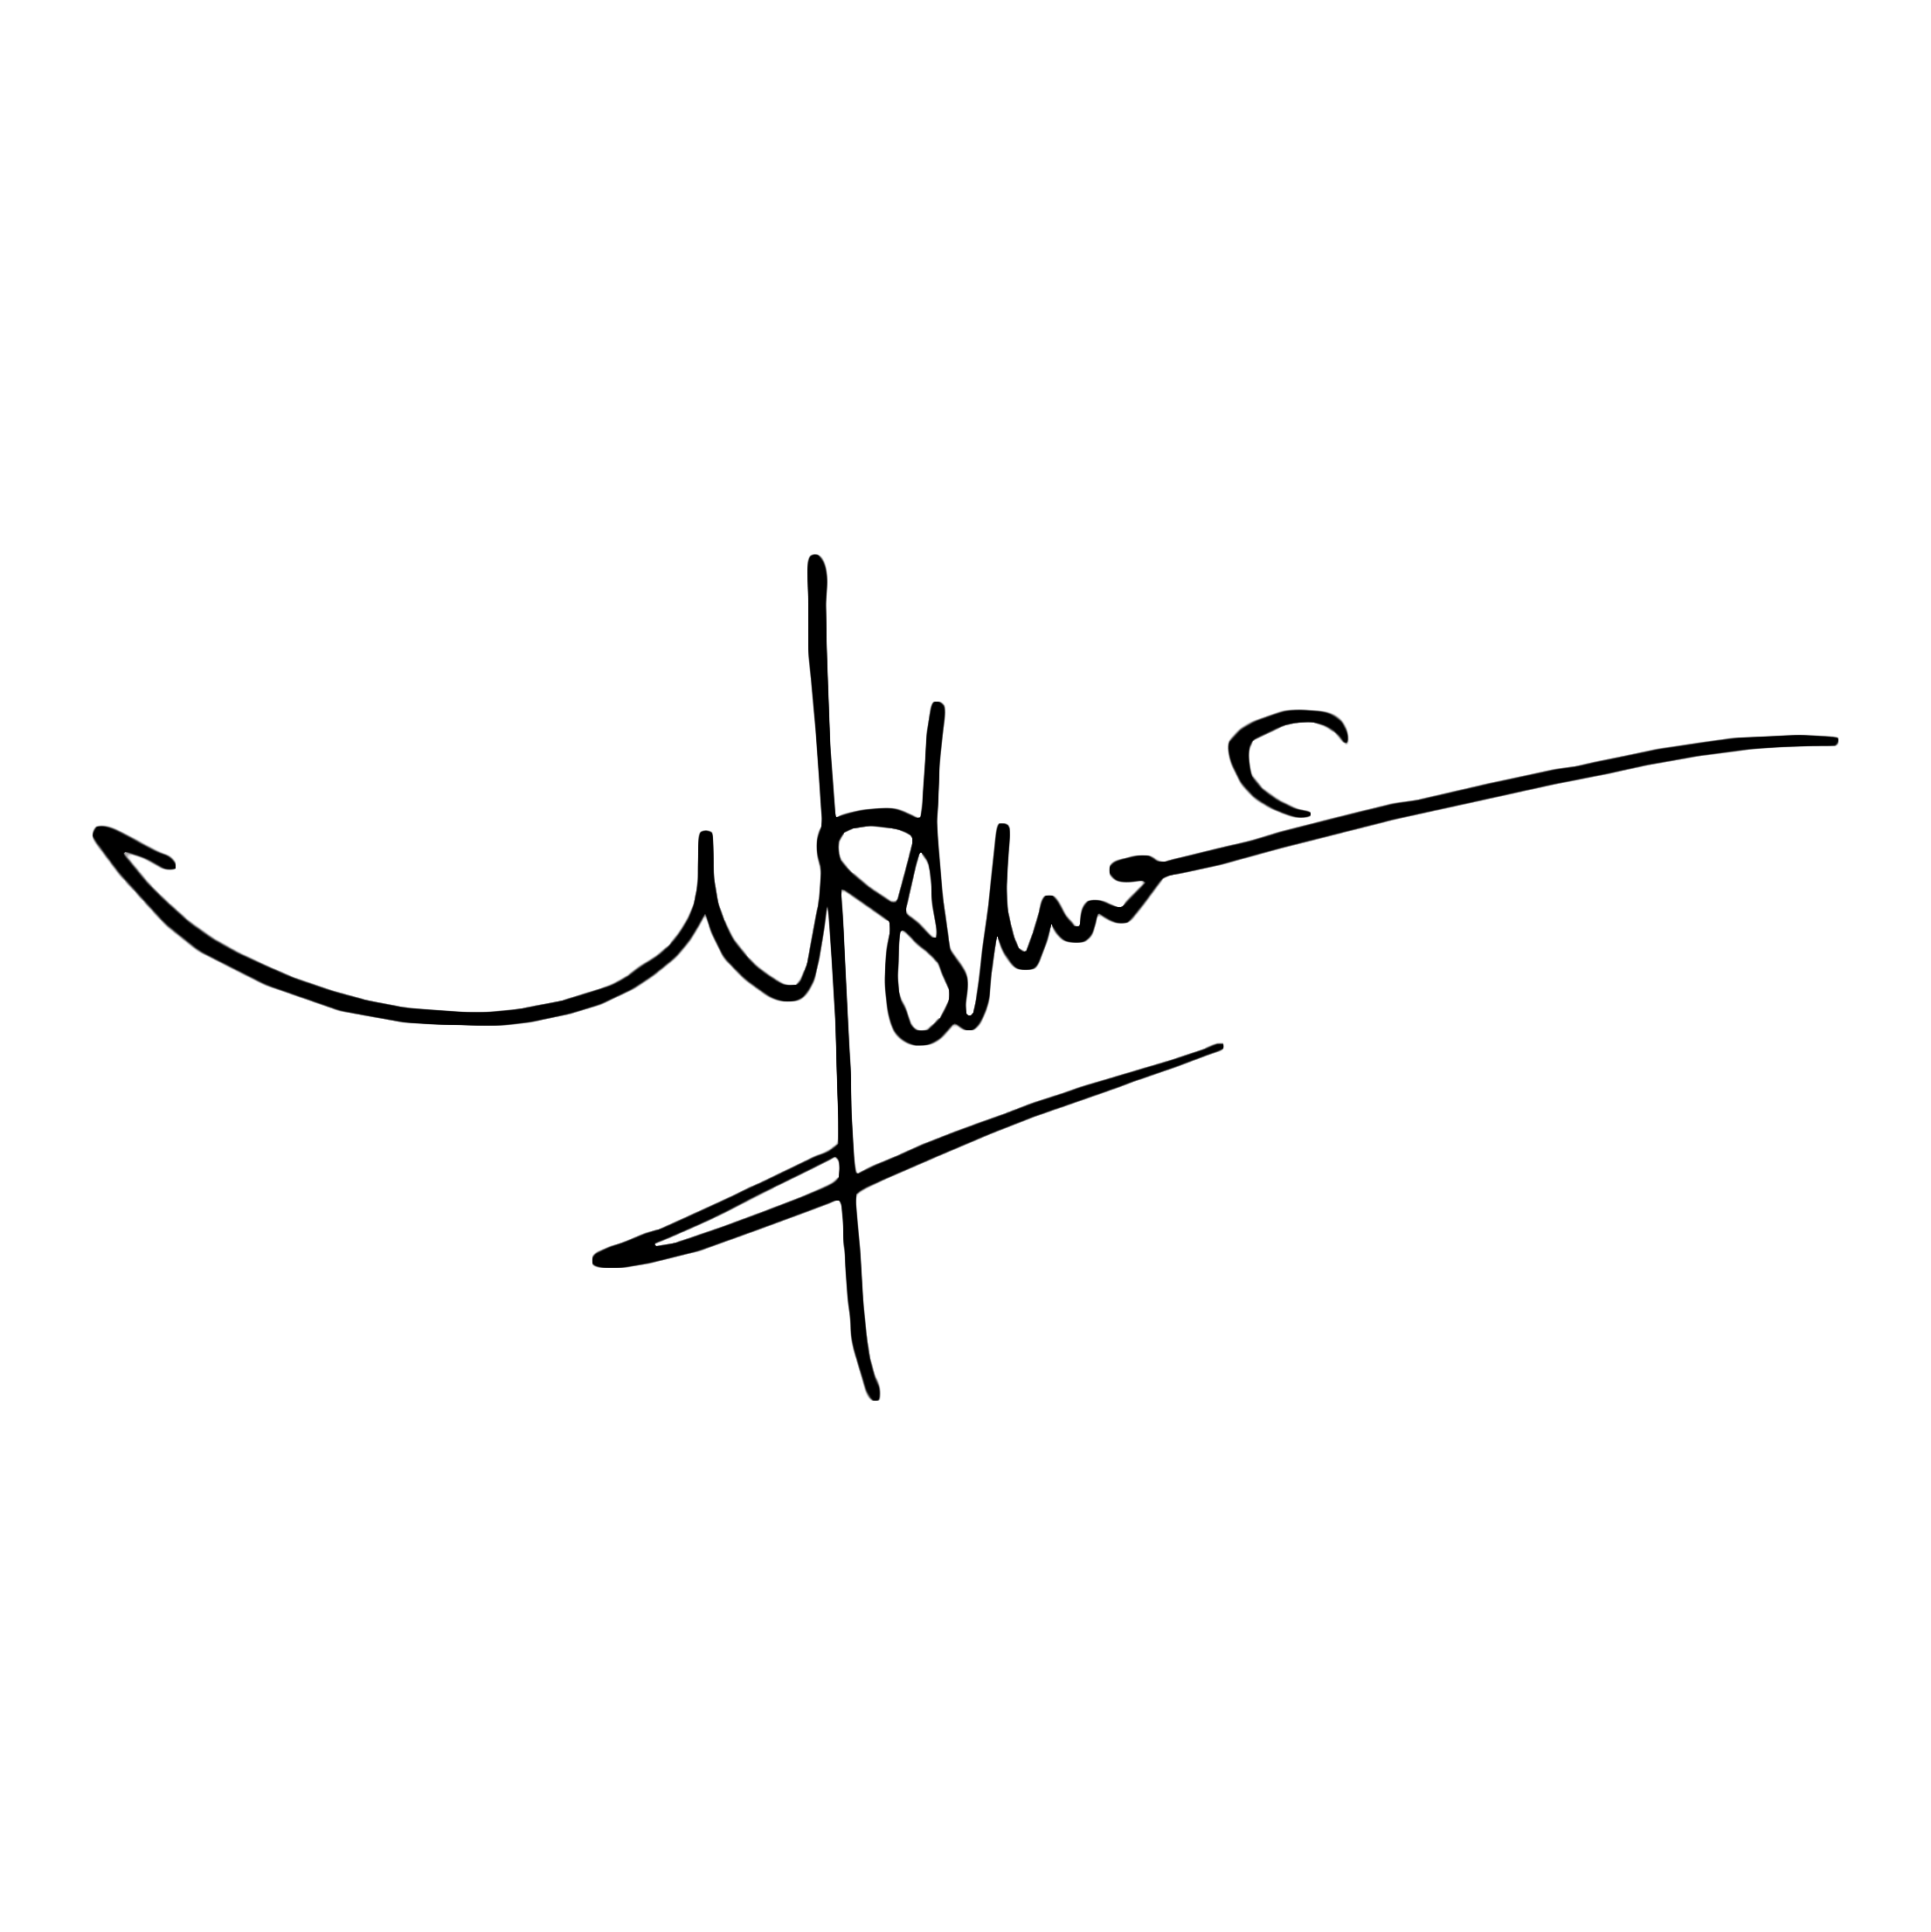
\includegraphics[width=3cm]{assets/pics/tanda_tangan_wikipedia.png}};
%\end{tikzpicture}

\begin{center}
	\bo{\type~ini adalah hasil karya saya sendiri, \\
	dan semua sumber baik yang dikutip maupun dirujuk \\
	telah saya nyatakan dengan benar.} \\
	\vspace*{2.6cm}

	\begin{tabular}{l c l}
	\bo{Nama} & : & \bo{\penulis} \\
	\bo{NPM} & : & \bo{\npm} \\
	\bo{Tanda Tangan} & : & \\
	& & \\
	& & \\
	\bo{Tanggal} & : & \bo{\tanggalSiapSidang} \\
	\end{tabular}
\end{center}

\newpage

	\forceclearchapter
}

% Memunculkan penomoran kembali
\pagenumbering{roman}

%
% setelah bagian ini, halaman dihitung sebagai halaman ke 2
\setcounter{page}{2}

%
% Lembar Penegesahan
\strcompare{Laporan Kerja Praktik}{\type}
{
	% Lembar Pengesahan Kerja Praktik dari LaTeX
	\addChapter{LEMBAR PERSETUJUAN DOSEN KERJA PRAKTIK}
	%
% Halaman Pengesahan Laporan Kerja Praktik
%
% @author  Andreas Febrian, Andre Tampubolon
% @version 2.1.2
% @edit by Ichlasul Affan
%

\chapter*{HALAMAN PERSETUJUAN DOSEN KERJA PRAKTIK}
\thispagestyle{empty}
\vspace*{0.4cm}
\noindent

\noindent
\begin{tabular}{ll p{9cm}}
	\multicolumn{3}{l}{\type~ini diajukan oleh:}  \\
	Nama&: & \penulis \\
	NPM&: & \npm \\
	Program Studi&: & \program \\
	Judul Kerja Praktik&: & \judul \\
\end{tabular} \\

\vspace*{1.0cm}

\noindent \bo{Telah berhasil diselesaikan laporan kerja praktik untuk
Fakultas \fakultas~dan dipresentasikan hasil kerja praktiknya sebagai
persyaratan yang harus dipenuhi dalam mata kuliah Kerja Praktik.}\\[0.2cm]

\begin{center}
	DOSEN MATA KULIAH KERJA PRAKTIK\\[2cm]
\end{center}

\begin{center}
	\underline{\pembimbingSatu}\\[0.1cm]
\end{center}

\vspace*{2.0cm}

\begin{tabular}{ll l}
	Ditetapkan di&: & Depok\\
	Tanggal&: & \tanggalLulus \\
\end{tabular}

\newpage

	\forceclearchapter
}
{
	\addChapter{LEMBAR PENGESAHAN}
	% Gunakan salah satu (comment atau hapus kode yang tidak perlu):
	% Lembar Pengesahan Tugas Akhir dari LaTeX
	\strcompare{Doktor}{\jenjang}
	{%
% Halaman Pengesahan Sidang (S3)
%
% @author  Andreas Febrian, Andre Tampubolon
% @version 2.1.2
% @edit by Ichlasul Affan
%

\chapter*{HALAMAN PENGESAHAN}
\thispagestyle{empty}
\vspace*{0.4cm}
\noindent

\noindent
\begin{tabular}{ll p{9cm}}
	\type~ini diajukan oleh&: & \\
	Nama&: & \penulis \\
	NPM&: & \npm \\
	Program Studi&: & \program \\
	Judul \type&: & \judul \\
\end{tabular} \\

\vspace*{1.0cm}

\noindent \bo{Telah berhasil dipertahankan di hadapan Dewan Penguji
dan diterima sebagai bagian persyaratan yang diperlukan untuk
memperoleh gelar Doktor pada Program Studi \program, Fakultas
\fakultas, Universitas Indonesia.}\\[0.2cm]

\begin{center}
	\bo{DEWAN PENGUJI}
\end{center}

\vspace*{0.3cm}

\def\blank{}
\begin{longtable}{l l p{7cm} l }
	\centering
	& & & \\
	Promotor&: & \pembimbingSatu & (\hspace*{3.0cm}) \\
	\ifx\blank\pembimbingDua
    \else
        & & & \\
    	Kopromotor&: & \pembimbingDua & (\hspace*{3.0cm}) \\
    \fi
    \ifx\blank\pembimbingTiga
    \else
        & & & \\
    	&: & \pembimbingTiga & (\hspace*{3.0cm}) \\
    \fi
	& & & \\
	Tim Penguji&: & \pengujiSatu~(Ketua) & (\hspace*{3.0cm}) \\
	& & & \\
	&: & \pengujiDua~(Anggota) & (\hspace*{3.0cm}) \\
	\ifx\blank\pengujiTiga
    \else
        & & & \\
    	&: & \pengujiTiga~(Anggota) & (\hspace*{3.0cm}) \\
    \fi
	\ifx\blank\pengujiEmpat
	\else
		& & & \\
		&: & \pengujiEmpat~(Anggota) & (\hspace*{3.0cm}) \\
	\fi
	\ifx\blank\pengujiLima
	\else
		& & & \\
		&: & \pengujiLima~(Anggota) & (\hspace*{3.0cm}) \\
	\fi
	\ifx\blank\pengujiEnam
	\else
		& & & \\
		&: & \pengujiEnam~(Anggota) & (\hspace*{3.0cm}) \\
	\fi
\end{longtable}

\vspace*{2.0cm}

\begin{tabular}{ll l}
	Ditetapkan di&: & Depok\\
	Tanggal&: & \tanggalLulus \\
\end{tabular}


\newpage
}
	{%
% Halaman Pengesahan Sidang
%
% @author  Andreas Febrian, Andre Tampubolon
% @version 2.1.2
% @edit by Muhammad Aulia Adil Murtito
%

\chapter*{HALAMAN PENGESAHAN}
\thispagestyle{empty}
\vspace*{0.4cm}
\noindent

\noindent
\begin{tabular}{ll p{9cm}}
	\type~ini diajukan oleh&: & \\
	Nama&: & \penulis \\
	NPM&: & \npm \\
	Program Studi&: & \program \\
	Judul \type&: & \judul \\
\end{tabular} \\

\vspace*{1.0cm}

\noindent \bo{Telah berhasil dipertahankan di hadapan Dewan Penguji
dan diterima sebagai bagian persyaratan yang diperlukan untuk
memperoleh gelar \jenjang~pada Program Studi \program, Fakultas
\fakultas, Universitas Indonesia.}\\[0.2cm]

\begin{center}
	\bo{DEWAN PENGUJI}
\end{center}

\vspace*{0.3cm}

\def\blank{}
\begin{tabular}{l l p{7cm} l }
	\centering
	& & & \\
	Pembimbing 1&: & \pembimbingSatu & (\hspace*{3.0cm}) \\
	\ifx\blank\pembimbingDua
    \else
        & & & \\
    	Pembimbing 2&: & \pembimbingDua & (\hspace*{3.0cm}) \\
    \fi
	& & & \\
	Penguji 1&: & \pengujiSatu & (\hspace*{3.0cm}) \\
	& & & \\
	Penguji 2&: & \pengujiDua & (\hspace*{3.0cm}) \\
	\ifx\blank\pengujiTiga
    \else
        & & & \\
    	Penguji 3&: & \pengujiTiga & (\hspace*{3.0cm}) \\
    \fi
\end{tabular}\\

\vspace*{2.0cm}

\begin{tabular}{ll l}
	Ditetapkan di&: & Depok\\
	Tanggal&: & \tanggalLulus \\
\end{tabular}


\newpage
}
	\forceclearchapter
	% Lembar Pengesahan dari PDF lain (misal: generated oleh SISIDANG [Fasilkom])
	%\putpdf{assets/pdfs/pengesahanSidang.pdf}
}


\strcompare{Laporan Kerja Praktik}{\type}{}
{
	%
	% Kata Pengantar
	\addChapter{\kataPengantar}
	%-----------------------------------------------------------------------------%
\chapter*{\kataPengantar}
%-----------------------------------------------------------------------------%
\pagestyle{first-pages}

I would like to express my gratitude to God Almighty, whom without His blessings and grace, I would not be able to write this thesis.

First of all, I am deeply grateful to my supervisor, Muhammad Hafizhuddin Hilman, S.Kom., M.Kom., Ph.D. for his guidance and support throughout the research process. I'm truly fortunate to have the opportunity to learn from him and gain valuable research experience.

I would also like to acknowledge the companies I've worked at, as they provided me with important technical and non-technical skills which were integral to the completion of this research project. Furthermore, I would like to thank my colleagues who have supported me throughout my academic studies. Lastly, I'm immensely grateful to my parents and sister for believing in me and for their unwavering support.

% Template ini disediakan untuk orang-orang yang berencana menggunakan \latex~untuk membuat dokumen tugas akhir.

% \todo{Silakan ganti pesan ini dengan pendahuluan kata pengantar Anda.}

% Ucapan Terima Kasih:
% \begin{enumerate}[topsep=0pt,itemsep=-1ex,partopsep=1ex,parsep=1ex]
% 	\item Pembimbing.
% 	\item Dosen.
% 	\item Instansi.
% 	\item Orang tua.
% 	\item Sahabat.
% 	\item Teman.
% \end{enumerate}

% Penulis menyadari bahwa laporan \type~ini masih jauh dari sempurna. Oleh karena itu, apabila terdapat kesalahan atau kekurangan dalam laporan ini, Penulis memohon agar kritik dan saran bisa disampaikan langsung melalui \f{e-mail} \code{emailanda@mail.id}.

% \begin{figure}
% 	\centering
% 	\includegraphics[width=0.74\textwidth]
% 	{assets/pics/creative_commons.png}
% 	\caption*{\license}
% 	\label{fig:lisensi}
% \end{figure}

% Terkait template ini, gambar lisensi di atas diambil dari \url{http://creativecommons.org/licenses/by-nc-sa/1.0/deed.en_CA}. Jika ingin mengentahui lebih lengkap mengenai \license, silahkan buka \url{http://creativecommons.org/licenses/by-nc-sa/1.0/legalcode}.
% Seluruh dokumen yang dibuat dengan menggunakan template ini sepenuhnya menjadi hak milik pembuat dokumen dan bebas didistribusikan sesuai dengan keperluan masing-masing.
% Lisensi hanya berlaku jika ada orang yang membuat template baru dengan menggunakan template ini sebagai dasarnya.

% Penyusun template ingin berterima kasih kepada Andreas Febrian, Lia Sadita, Fahrurrozi Rahman, Andre Tampubolon, dan Erik Dominikus atas kontribusinya dalam template yang menjadi pendahulu template ini.
% Penyusun template juga ingin mengucapkan terima kasih kepada Azhar Kurnia atas kontribusinya dalam template yang menjadi pendahulu template ini.

% Semoga template ini dapat membantu orang-orang yang ingin mencoba menggunakan \latex.
% Semoga template ini juga tidak berhenti disini dengan ada kontribusi dari para penggunanya.
% Jika Anda memiliki perubahan yang dirasa penting untuk disertakan dalam template, silakan lakukan \f{fork} repositori Git template ini di \url{https://gitlab.com/ichlaffterlalu/latex-skripsi-ui-2017}, lalu lakukan \f{merge request} perubahan Anda terhadap \f{branch} \code{master}.
% Kami berharap agar \f{template} ini dapat terus diperbarui mengikuti perubahan ketentuan dari pihak Rektorat Universitas Indonesia, dan hal itu tidak mungkin terjadi tanpa kontribusi dari teman-teman sekalian.

% Untuk input gambar tanda tangan, silahkan sesuaikan xshift, yshift, dan width dengan gambar tanda tangan Anda
%\begin{tikzpicture}[remember picture,overlay,shift={(current page.north east)}]
%\node[anchor=north east,xshift=-3cm,yshift=-6.2cm]{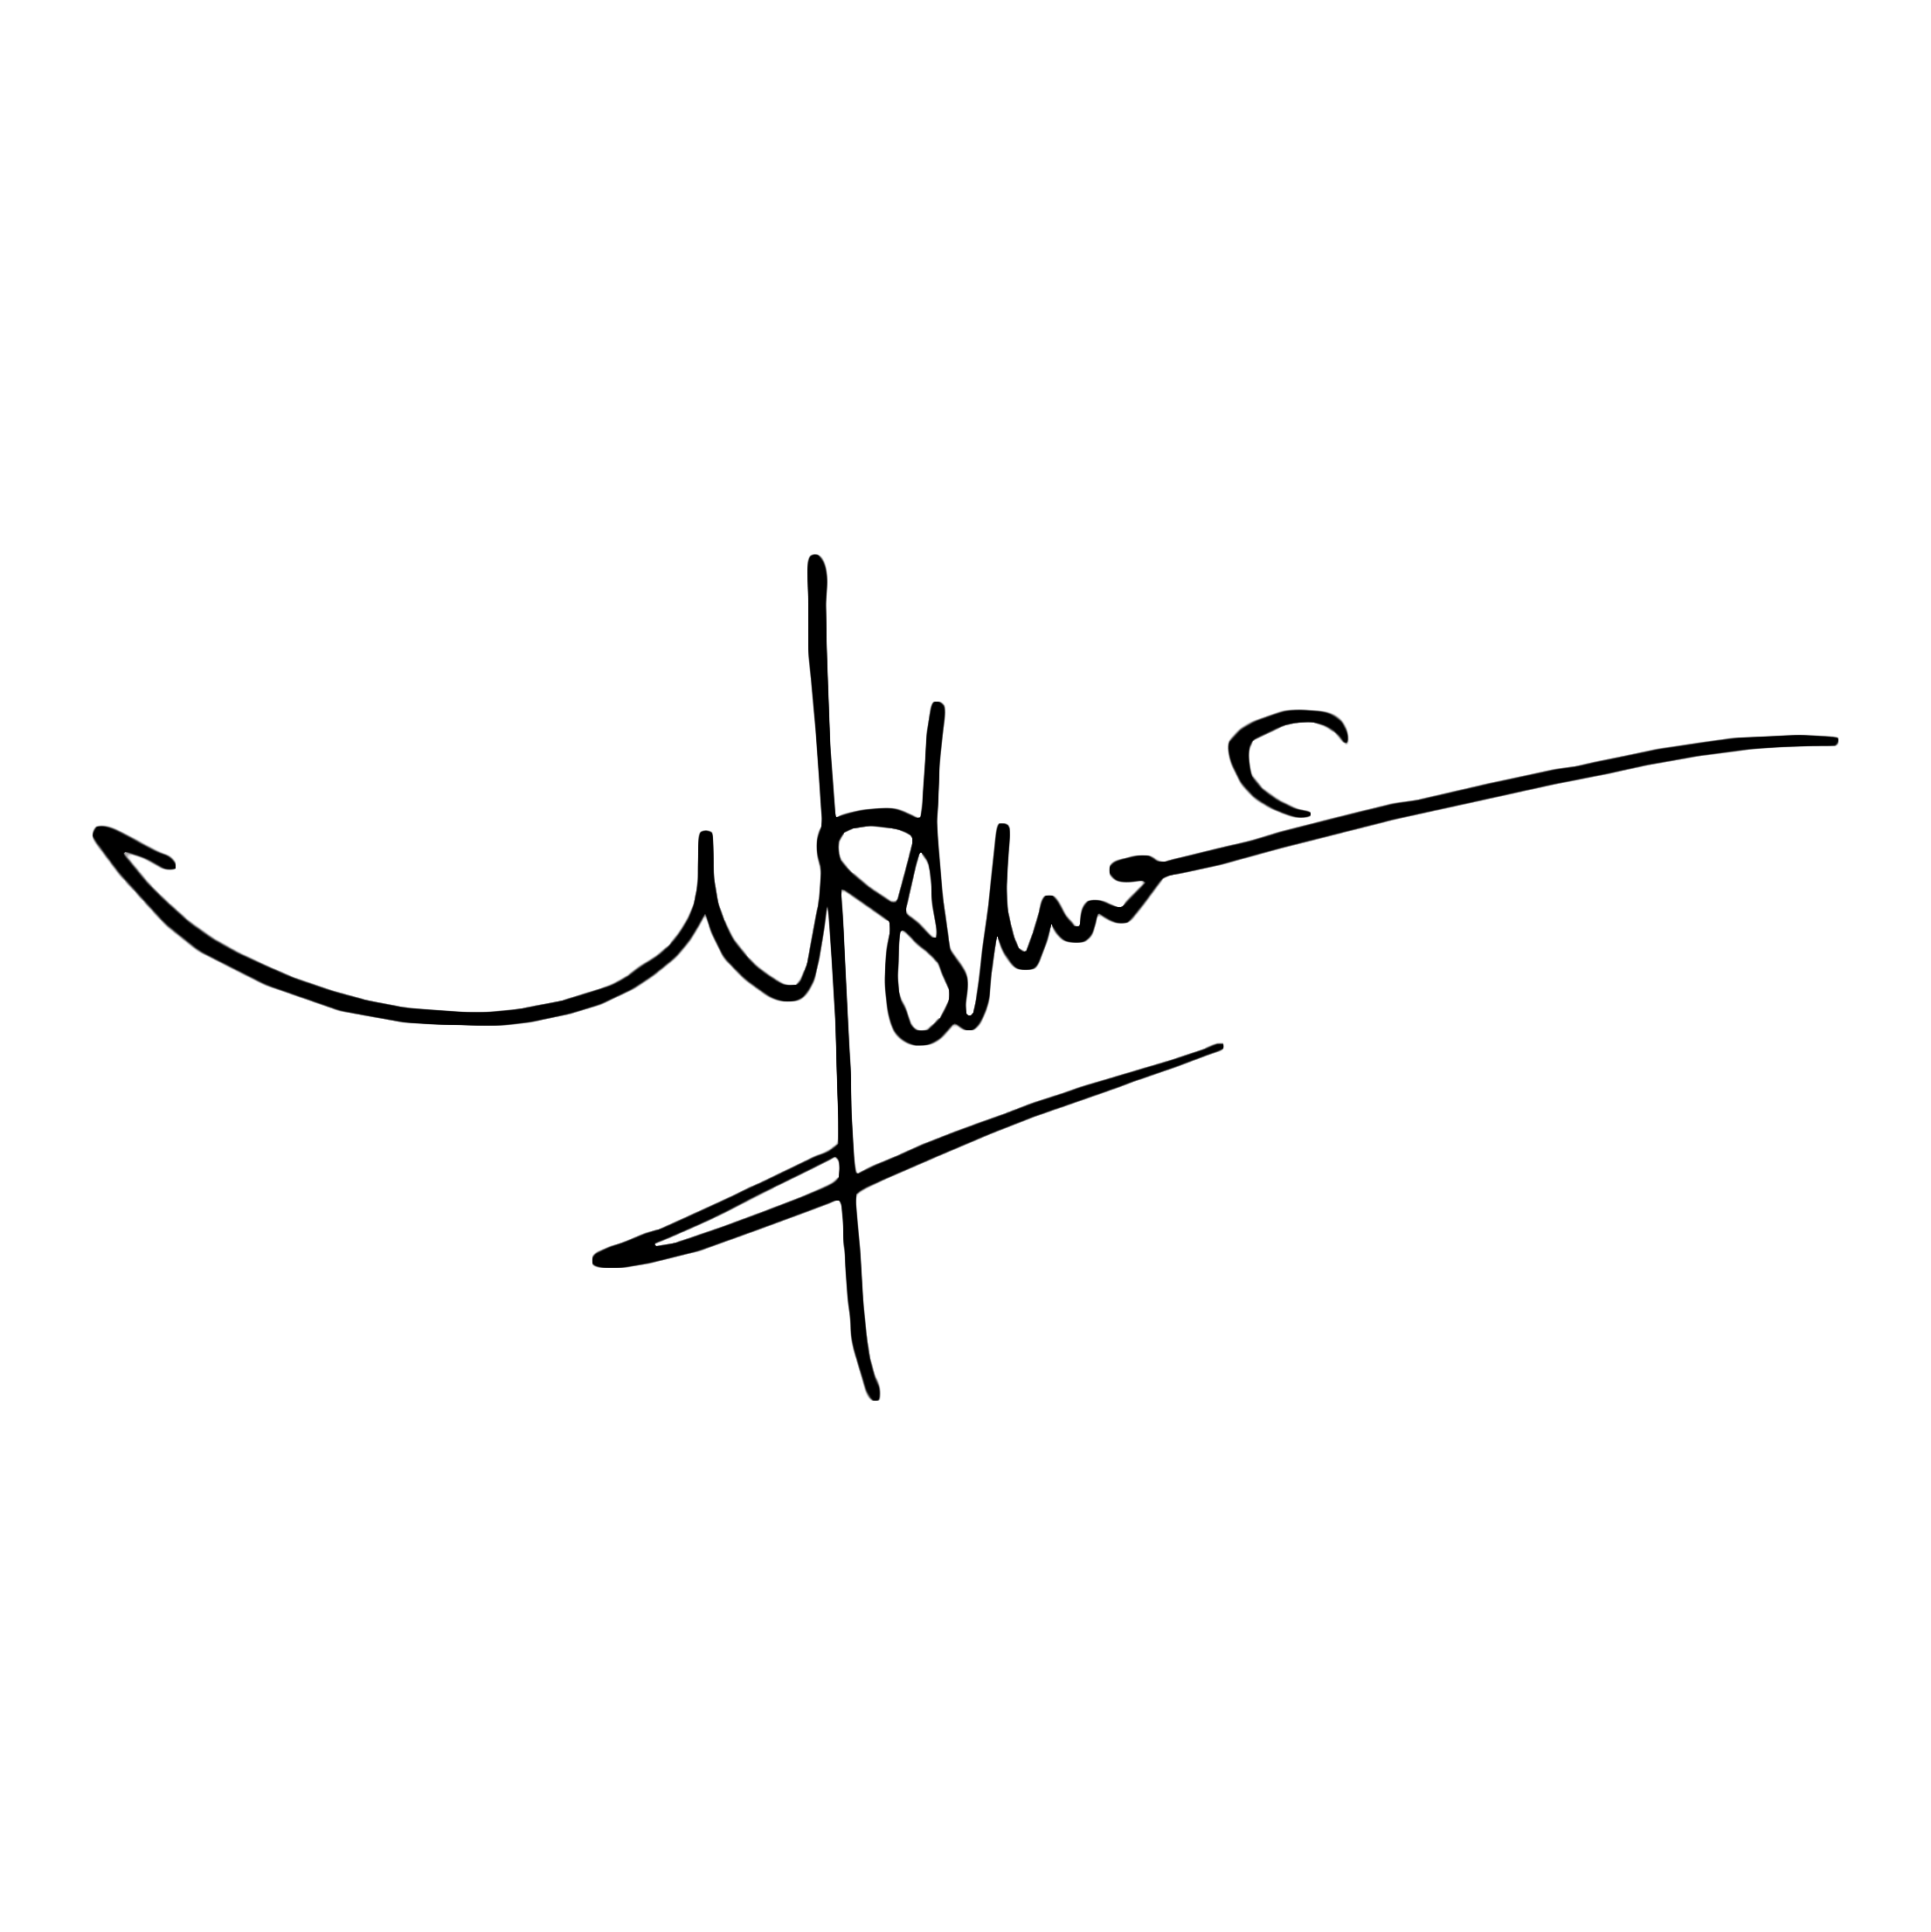
\includegraphics[width=3cm]{assets/pics/tanda_tangan_wikipedia.png}};
%\end{tikzpicture}

\vspace*{0.1cm}
\begin{flushright}
Depok, \tanggalSiapSidang\\[0.1cm]
\vspace*{1.5cm}
\penulis

\end{flushright}

	\forceclearchapter
	%
	% Lembar Persetujuan Publikasi Ilmiah
	\addChapter{LEMBAR PERSETUJUAN PUBLIKASI ILMIAH}
	%
% @author  Andre Tampubolon, Andreas Febrian
% @version 2.1.2
% @edit by Muhammad Aulia Adil Murtito
%

\chapter*{\uppercase{Halaman Pernyataan Persetujuan Publikasi Tugas Akhir untuk Kepentingan Akademis}}
\thispagestyle{empty}
\vspace*{0.2cm}
\noindent
Sebagai sivitas akademik Universitas Indonesia, saya yang bertanda
tangan di bawah ini:
\vspace*{0.4cm}


\begin{tabular}{p{4.2cm} l p{6cm}}
	\bo{Nama} & : & \penulis \\
	\bo{NPM} & : & \npm \\
	\bo{Program Studi} & : & \program\\
	\bo{Fakultas} & : & \fakultas\\
	\bo{Jenis Karya} & : & \type \\
\end{tabular}

\vspace*{0.6cm}
\noindent demi pengembangan ilmu pengetahuan, menyetujui untuk memberikan
kepada Universitas Indonesia \bo{Hak Bebas Royalti Noneksklusif
(\textit{Non-exclusive Royalty Free Right})} atas karya ilmiah saya yang berjudul:
\begin{center}
	\judul
\end{center}
beserta perangkat yang ada (jika diperlukan). Dengan Hak Bebas Royalti
Noneksklusif ini Universitas Indonesia berhak menyimpan,
mengalihmedia/formatkan, mengelola dalam bentuk pangkalan data
(\textit{database}), merawat, dan memublikasikan tugas akhir saya selama
tetap mencantumkan nama saya sebagai penulis/pencipta dan sebagai
pemilik Hak Cipta. \\

\noindent Demikian pernyataan ini saya buat dengan sebenarnya.

% Untuk input gambar tanda tangan, silahkan sesuaikan xshift, yshift, dan width dengan gambar tanda tangan Anda
%\begin{tikzpicture}[remember picture,overlay,shift={(current page.north east)}]
%\node[anchor=north east,xshift=-9cm,yshift=-23.5cm]{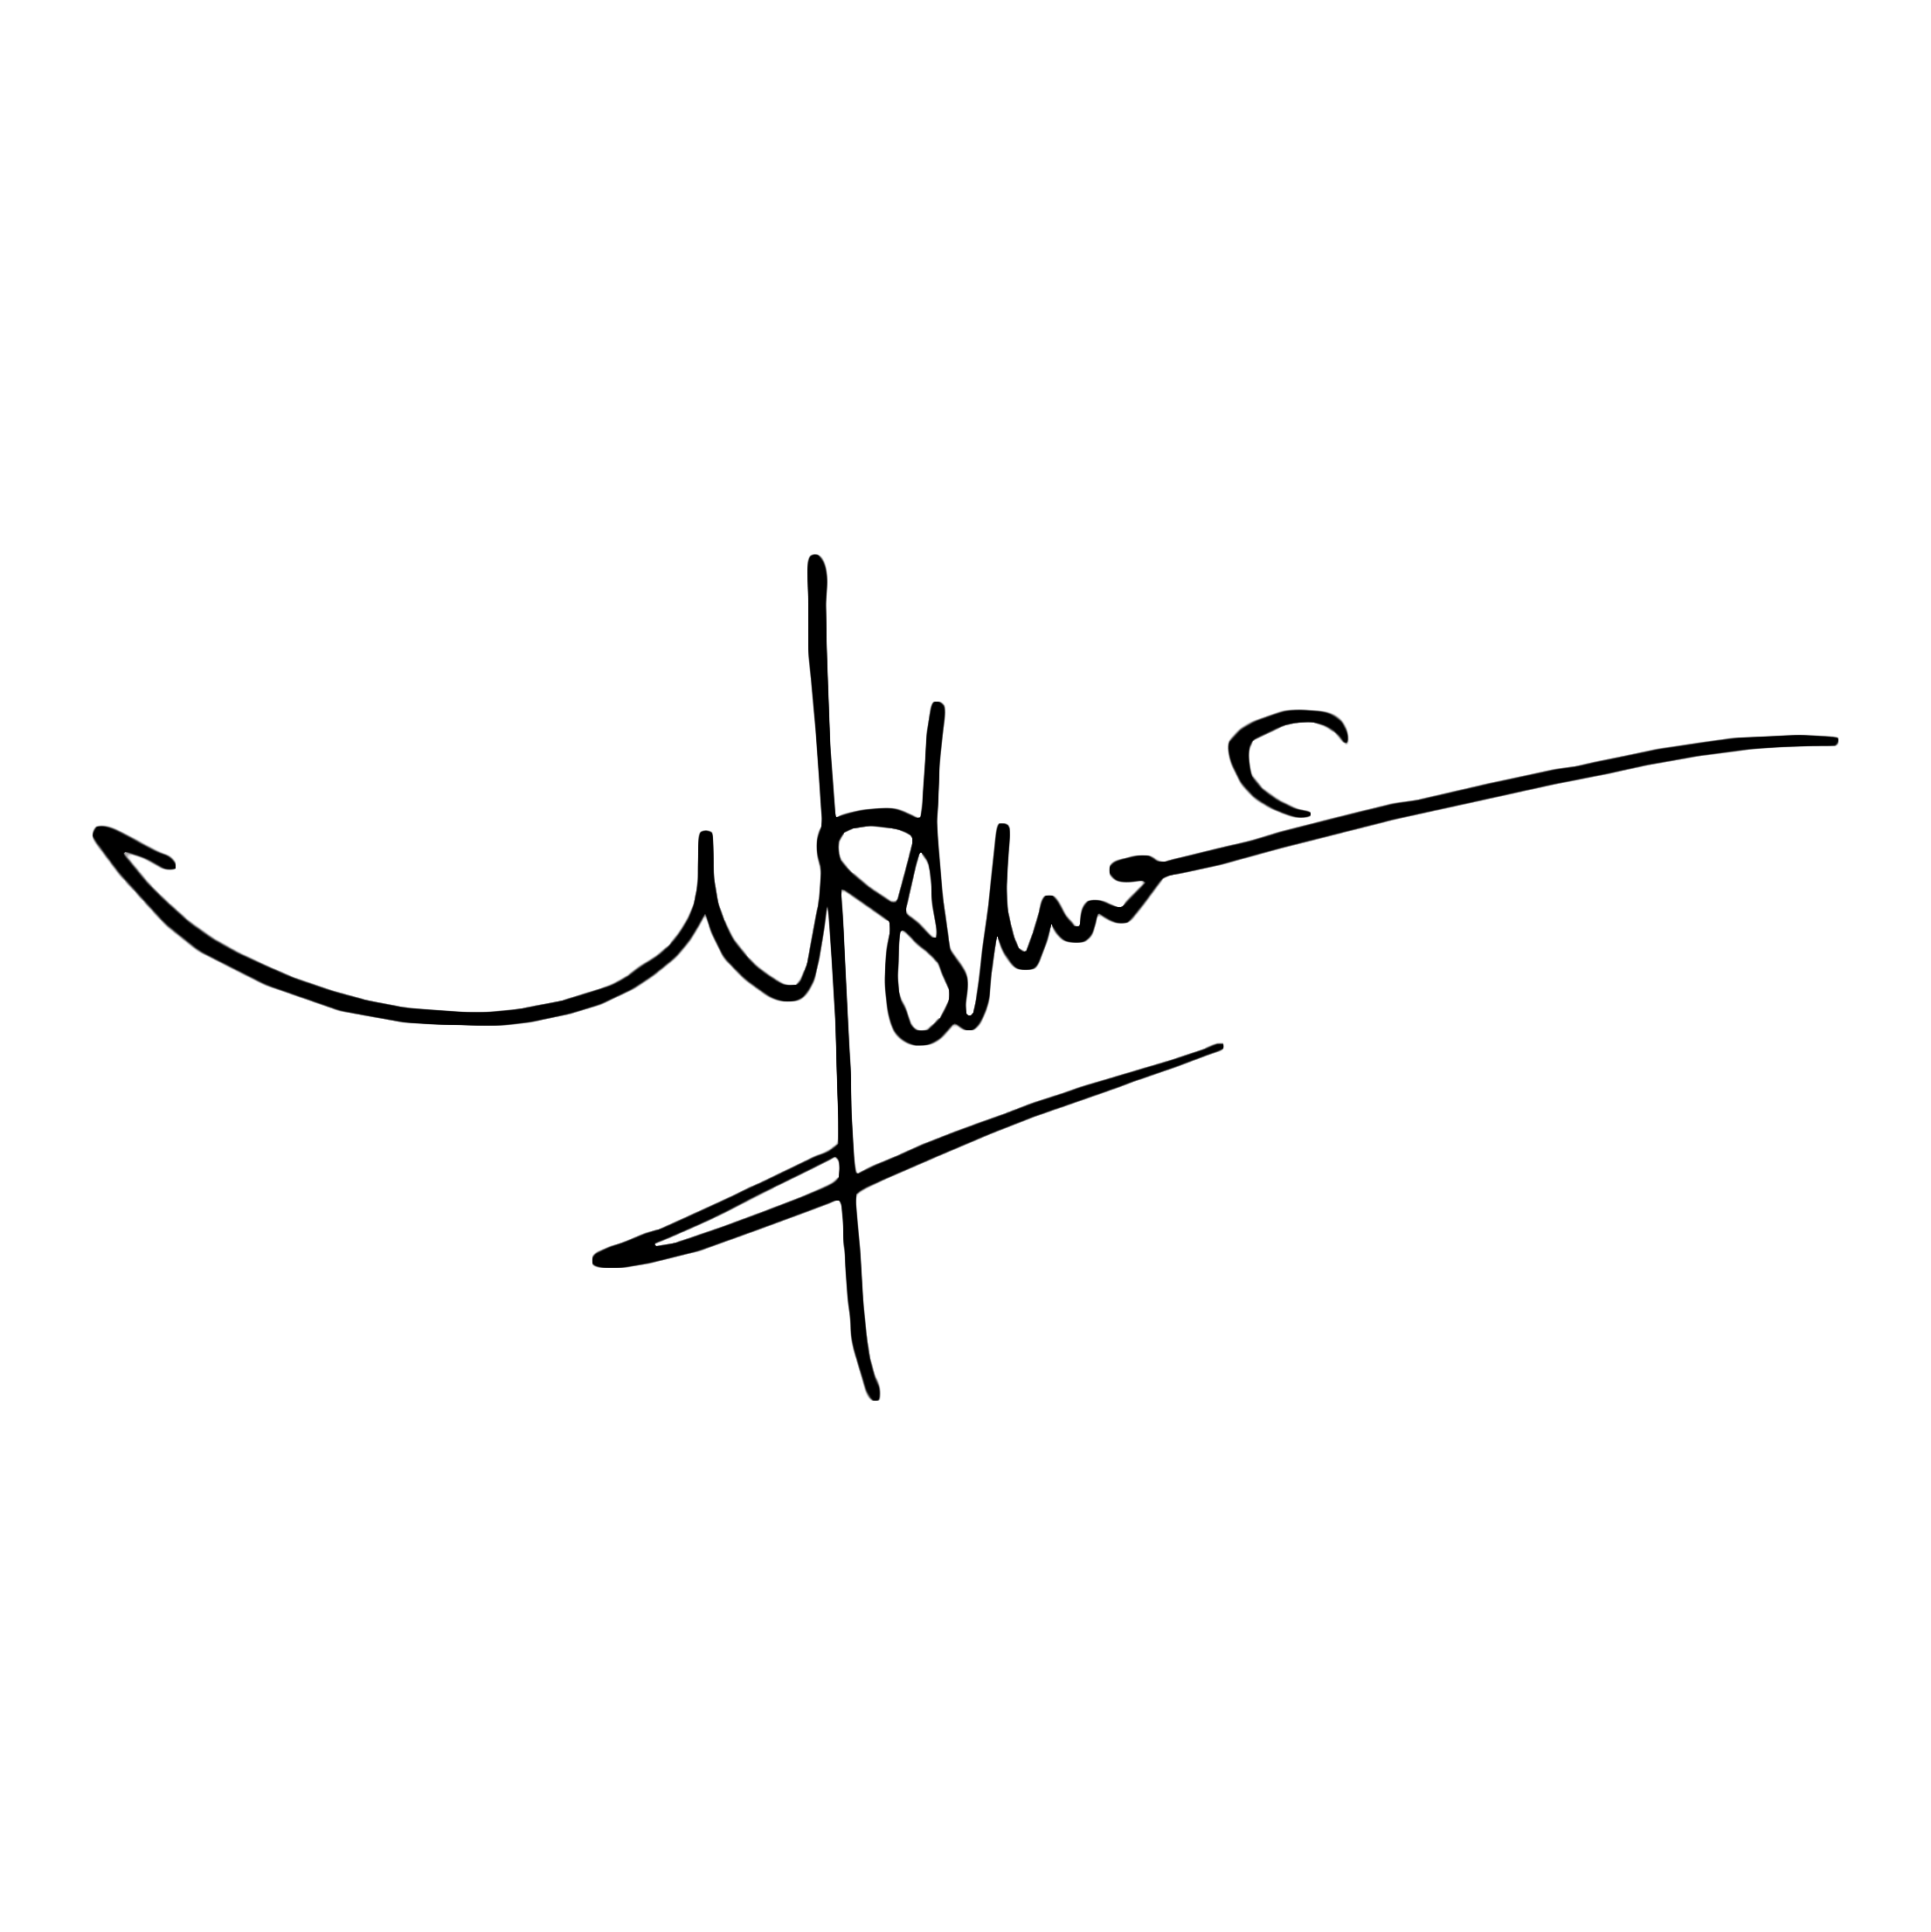
\includegraphics[width=3cm]{assets/pics/tanda_tangan_wikipedia.png}};
%\end{tikzpicture}

\begin{center}
	\vspace*{0.8cm}
	\begin{tabular}{lll}
		Dibuat di&: & Depok \\
		Pada tanggal&: & \tanggalSiapSidang \\
	\end{tabular}\\

	\vspace*{0.2cm}
	Yang menyatakan \\
	\vspace*{2cm}
	(\penulis)
\end{center}

\newpage

	\forceclearchapter
}

%
% Untuk halaman pertama setiap chapter mulai dari abstrak, tetap berikan mark universitas.
%
\pagestyle{first-pages}

%
\addChapter{ABSTRAK}
%
% Halaman Abstrak
%
% @author  Andreas Febrian
% @version 2.1.2
% @edit by Ichlasul Affan
%

\chapter*{Abstrak}
\singlespacing

\vspace*{0.2cm}

% Untuk conditional statement pembimbing dua
\def\blank{}

\noindent \begin{tabular}{l l p{10cm}}
	Nama&: & \penulis \\
	Program Studi&: & \program \\
	Judul&: & \judul \\
	Pembimbing&: & \pembimbingSatu \\
	\ifx\blank\pembimbingDua
    \else
        \ &\ & \pembimbingDua \\
    \fi
    \ifx\blank\pembimbingTiga
    \else
    	\ &\ & \pembimbingTiga \\
    \fi
\end{tabular} \\

\vspace*{0.5cm}

% \noindent Dengan kebutuhan untuk menyediakan layanan kepada pengguna di seluruh dunia yang terus berkembang, layanan aplikasi web harus berdaptasi menggunakan teknologi baru untuk memenuhi kebutuhan ini.

% Namun, ada kelangkaan studi mengenai metode \textit{geo-distributed clusters} dan kinerjanya. Oleh karena itu,

\noindent Kebutuhan untuk menyediakan layanan kepada pengguna di seluruh dunia menyebabkan layanan aplikasi web untuk berdaptasi menggunakan teknologi baru dan memadai. Untuk mencapai hal tersebut, layanan cloud servis digunakan untuk memperluas jangkauan geografis dari layanan web di seluruh dunia. Peningkatan kualitas pengembangan \textit{deployment} aplikasi web terlihat pada Kubernetes, alat yang diadopsi secara luas yang didukung di sebagian besar platform cloud, yang memungkinkan penerapan \textit{geo-distributed clusters} untuk aplikasi yang memiliki pengguna multinasional. Dikarenakan kelangkaan studi mengenai \textit{geo-distributed clusters} dan kinerjanya, penelitian ini bermaksud untuk menjembatani kesenjangan pengetahuan tersebut dengan mengimplementasikan solusi menggunakan Istio (Anthos Service Mesh), mesh layanan yang paling banyak digunakan untuk aplikasi Kubernetes, serta solusi cloud native di Google Cloud Platform menggunakan MultiClusterService. Studi ini menemukan bahwa kedua pendekatan tersebut dapat diandalkan, namun, Istio/ASM memiliki latensi yang sedikit lebih rendah untuk sebagian besar \textit{request}. Kedua pendekatan tersebut merupakan pilihan baik untuk aplikasi global, karena keduanya menggunakan \textit{geo-aware load balancing}, yang merutekan permintaan pengguna ke klaster terdekat yang tersedia. Basis kode studi dan hasil pengujian ini tersedia secara \textit{open-sourced} untuk studi lebih lanjut tentang aplikasi berbasis \textit{geo-distributed Kubernetes clusters}.\\

\vspace*{0.2cm}

\noindent Kata kunci: \\ Kubernetes, Google Cloud Platform, MultiClusterService, Istio, Anthos Service Mesh \\

\setstretch{1.4}
\newpage

%
%
%
% Halaman Abstract
%
% @author  Andreas Febrian
% @version 2.1.2
% @edit by Ichlasul Affan
%

\chapter*{ABSTRACT}
\singlespacing

\vspace*{0.2cm}

% Untuk conditional statement pembimbing dua
\def\blank{}

\noindent \begin{tabular}{l l p{11.0cm}}
	Name&: & \penulis \\
	Study Program&: & \studyProgram \\
	Title&: & \judulInggris \\
	Counsellor&: & \pembimbingSatu \\
	\ifx\blank\pembimbingDua
	\else
		\ &\ & \pembimbingDua \\
	\fi
	\ifx\blank\pembimbingTiga
	\else
		\ &\ & \pembimbingTiga \\
	\fi
\end{tabular} \\

\vspace*{0.5cm}

\noindent With the need of providing services to ever-growing worldwide users, web application services must adapt new technologies in order to fulfill these needs. As setting up physical servers across the globe is a daunting task, cloud service providers are an essential tool to reach geographical coverage for worldwide web services. Further advancements on the developer experience of deploying web applications can be seen in tools such as Kubernetes, a widely adopted tool that's supported in most cloud platforms that enables the implementation of geo-distributed clusters for applications with a multi-national user base. However, there is a scarcity of studies regarding geo-distributed clusters methods and its performance. Therefore, this study intends to bridge that knowledge gap by implementing a solution using Istio (Anthos Service Mesh), the most used service mesh for kubernetes applications as well as a cloud native solution on Google Cloud Platform using MultiClusterService. This study found that both approaches are reliable, however, Istio / ASM has a slightly lower latency for the vast majority of requests. In addition, both approaches are a viable choice for worldwide applications, as they both use geo-aware load balancing, which routes user requests to the nearest available cluster. This study's scripts and test results are open-sourced for further studies about geo-distributed Kubernetes-based applications.\\

\vspace*{0.2cm}

\noindent Key words: \\ Kubernetes, Google Cloud Platform, MultiClusterService, Istio, Anthos Service Mesh \\

\setstretch{1.4}
\newpage


%
% Daftar isi, gambar, tabel, dan kode
%
\CAPinToC % All entries in ToC will be CAPITALIZED from here on
\phantomsection %hack to make them clickable
\singlespacing
\tableofcontents
\setstretch{1.4}
\clearpage
\phantomsection %hack to make them clickable
\singlespacing
\listoffigures
\setstretch{1.4}
\clearpage
\phantomsection %hack to make them clickable
\singlespacing
\listoftables
\setstretch{1.4}
\clearpage

%
% Daftar Kode Program
% Comment to disable.
%
\phantomsection %hack to make them clickable
\addcontentsline{toc}{chapter}{\lstlistlistingname}
\singlespacing
\listoflistings
\setstretch{1.4}
\clearpage

%
% Daftar Isi yang Didefinisikan Sendiri (Custom)
% Definisi jenis objek baru dapat dilakukan di uithesis.sty
% Uncomment to use.
%
%\phantomsection %hack to make them clickable
%\addcontentsline{toc}{chapter}{\listofthingname}
%\singlespacing
%\listofthing
%\setstretch{1.4}
%\clearpage

%
% Daftar Equation (Persamaan Matematis)
% Uncomment to use.
%
% \phantomsection %hack to make them clickable
% \addcontentsline{toc}{chapter}{\listofequname}
% \singlespacing
% \listofequ
% \setstretch{1.4}
% \clearpage

%
% Daftar Lampiran
% Comment to disable.
%
\phantomsection %hack to make them clickable
\addcontentsline{toc}{chapter}{\listofappendixname}
\singlespacing
\listofappendix
\setstretch{1.4}

% Table of content normal lagi hurufnya
\enableboldchapterintoc

\clearpage

% Jika penomoran romawi selesai di ganjil
%\naiveoddclearchapter
% Jika penomoran romawi selesai di genap
%\naiveevenclearchapter

\noCAPinToC % Revert to original \addcontentsline formatting

%
% Gunakan penomeran Arab (1, 2, 3, ...) setelah bagian ini.
%
\pagenumbering{arabic}
\pagestyle{standard}
% \setlength{\belowcaptionskip}{+2pt}



\setoddevenheader
%-----------------------------------------------------------------------------%
\chapter{\babSatu}
\label{bab:1}
%-----------------------------------------------------------------------------%
% Pada bab ini, akan dijelaskan tentang latar belakang dan permasalahan yang diselesaikan pada penelitian ini.
This chapter discusses the background, problem definition, research objectives, research scopes, and writing systematics. The goal of this chapter is to describe the background of the research topic and the problem that is intended to be solved while defining objectives, scopes, and writing systematics as a guide for this research.

%-----------------------------------------------------------------------------%
\section{Background}
\label{sec:background}
%-----------------------------------------------------------------------------%
% \todo{Tentukan latar belakang dari penelitian Anda di sini (\f{background}).}
The number of internet users increases every year with approximately 5.3 billion users in 2023 \citep{cisco-2020}. In anticipation of such growth, applications which serve users from all over the globe must be able to handle those kinds of traffic. Therefore, to handle traffic from different parts of the globe with high performance, multiple servers are deployed in multiple regions of the globe. An on-premise server approach introduces multiple complexities such as hardware and maintenance costs for every single physical machine. A simpler approach is to use a cloud-based service such as Google Cloud Platform.

% insert gcp explanation here
Google Cloud Platform (GCP) is a cloud computing service that offers a wide range of technical solutions to help aid the development and deployment of web applications. One of the services that Google Cloud Platform provides is Google Kubernetes Engine, a cloud solution for containerized applications using Kubernetes. Kubernetes is an open-source platform that provides an abstraction of containers and simplifies deploying, monitoring, and scaling a web-based application. Containerized applications improve the developer experience as developers do not need to worry about the deployment process and instead can focus entirely on application development \citep{xie-2020}. 

Kubernetes on the cloud offers a solution for applications with an international user base called geo-distributed clusters. Geo-distributed clusters are Kubernetes clusters that are spread across the world in order to minimize the latency of server response by reducing the physical distance between a user and the server, thus creating a better user experience. In a geo-distributed cluster configuration, traffic handling is done by a load balancer. The load balancer ideally distributes traffic efficiently to Kubernetes clusters. Kubernetes clusters are chosen based on several factors such as request-to-response distance, cluster workload (CPU) percentage, and many more. However, according to \citet{andrew-2023}, Google Cloud's load balancer does not handle geo-distributed applications very well. Therefore, there is a need to explore other load-balancing options that can work on a cloud-based application. An alternative is to use a service mesh.

% There are several ways of creating a multi-cluster infrastructure with Kubernetes on GCP, this study will look into two of those approaches: MultiClusterService with MultiClusterIngress and using Istio Serice Mesh.

% For a multi-cluster multi-region application, we can configure a Multi-Cluter Service to register services into a cluster set and handle traffic through a Multi-Cluster Ingress.

%--------------------------------------------- efficiently, --------------------------------%
% \section{Problem}
% \label{sec:problem}
%-----------------------------------------------------------------------------%

A service mesh is an infrastructure layer used to manage communication between services. A major benefit of using service mesh is a more configurable load balancing which has the upside of having locality-aware load balancing which is a load balancer that routes a user to the closest server. Three of the service mesh with the most stars on GitHub are Istio, Consul, and Linkerd respectively. As the purpose of this study is not to compare different service meshes, Istio is chosen for being supported by the Google Cloud Platform under the name of Anthos Service Mesh. Istio is a service mesh compatible with existing Kubernetes clusters. Istio offers locality-aware load balancing that considers the incoming request's geographical location to determine which server clusters are used to process the response with the goal of increasing the performance of web applications.

%-----------------------------------------------------------------------------%
\section{Problem Definition}
\label{sec:definisiMasalah}
%-----------------------------------------------------------------------------%

This research has the following problem definition:
\begin{itemize}
	% \item How does load balancing affect the performance of worldwide applications?
    % \item How does locality load balancing affect worldwide application performance?
    \item How does a geo-distributed cluster architecture improve the reliability of worldwide applications?
    \item How does the Istio approach improve application performance?
\end{itemize}



%-----------------------------------------------------------------------------%
\section{Research Objectives}
\label{sec:tujuan}
%-----------------------------------------------------------------------------%
This research has the following objectives:
\begin{itemize}
	\item To implement and evaluate the effects of google cloud load balancing on the performance of a worldwide application.
    \item To implement and evaluate the effects of locality load balancing on the performance of a worldwide application.
\end{itemize}

\section{Research Scopes}
\label{sec:batasanMasalah}
%-----------------------------------------------------------------------------%
This research has the following scopes:

\begin{itemize}
	\item Application performance testing in multi-region geo-distributed clusters is limited to simple web service applications.
    \item Multi-region geo-distributed cluster testing is limited to the cloud platform by Google Cloud Platform (GCP).
\end{itemize}
%-----------------------------------------------------------------------------%
% \section{Posisi Penelitian}
% \label{sec:posisiPenelitian}
% %-----------------------------------------------------------------------------%
% \todo{Sebutkan posisi penelitian Anda. Ada baiknya jika Anda menggunakan gambar atau diagram. Template ini telah menyediakan contoh cara memasukkan gambar.}

% \begin{figure}
% 	\centering
% 	
\includegraphics[width=0.4\textwidth]{assets/pics/makara.png}
% 	\caption{Penjelasan singkat terkait gambar.}
% 	\label{fig:research_position}
% \end{figure}

% \todo{Jelaskan \pic~\ref{fig:research_position} di sini.}


%-----------------------------------------------------------------------------%

% Berikut ini adalah langkah penelitian yang telah dilakukan:
% \begin{enumerate}
% 	\item Tinjauan literatur \\
% 	Pada tahap ini, dipelajari teori-teori yang terkait dengan penelitian ini untuk mendapatkan konsep dasar yang dibutuhkan dalam mencapai tujuan penelitian.
% 	\item Analisis implementasi dan kesimpulan \\
% 	Pada tahap ini, digunakan studi kasus untuk analisis terkait kegunaan \f{template}. Setelah melakukan analisis tersebut, ditarik kesimpulan keseluruhan dari penelitian ini.
% \end{enumerate}


%-----------------------------------------------------------------------------%
\section{Writing Systematics}
\label{sec:sistematikaPenulisan}
%-----------------------------------------------------------------------------%
The research report consists of six chapters, namely the introduction, literature review, methodology, implementation, results and analysis, and conclusions. The following are the descriptions of each chapter,
\begin{itemize}
	\item Chapter 1 \babSatu \\
	    This chapter is the introduction to this research which consists of the background, problem definition, research objectives, research scopes, and writing systematics.
	\item Chapter 2 \babDua \\
            This chapter discusses the theoretical foundation of this study from literature reviews to bridge the gap between theory and practice.
	\item Chapter 3 \babTiga \\
	    This chapter discusses the research methodology which includes research stages, application infrastructure design, testing scenarios, and evaluation metrics.
	\item Chapter 4 \babEmpat \\
		This chapter discusses the implementation of the application which is then deployed according to the test scenarios.
	\item Chapter 5 \babLima \\
	    This chapter discusses the findings from the experiments and presents the analysis from each of the test scenarios.
	\item Chapter 6 \kesimpulan \\
	    This chapter discusses the conclusion of this research as well as suggestions for future research.    
\end{itemize}

% \todo{Anda bisa mengubah atau menambahkan penjelasan singkat mengenai isi masing-masing bab. Setiap tugas akhir pasti ada yang berbeda pada bagian ini.}

\clearchapter
%-----------------------------------------------------------------------------%
\chapter{\babDua}
\label{bab:2}
%-----------------------------------------------------------------------------%
This chapter displays the results of the literature study that has been done to help further the research. The literature study is based on relevant topics that are used in this research.


%-----------------------------------------------------------------------------%
\section{Kubernetes}
\label{sec:kubernetes}
Kubernetes is used to manage, monitor, and scale containers of a cluster and can be extended to geo-distributed clusters when hosted on a cloud platform. At first, application deployment is done by hosting the application on a dedicated machine on-premise. This changed when Cloud providers were introduced, where Cloud-based services helped improve deployment management through monitoring and scalability through cloud servers, removing the need of maintaining a physical server. The deployment process itself did not change much until a breakthrough in the form of Docker containers was introduced in 2010. 

Docker utilizes virtual machines that offer consistency and reliability, regardless of which machine it's being hosted on. This means that application behavior is consistent regardless of the machine itself as long as it is capable of running Docker. Docker's containerization solution, however, is limited to a single application. In reality, a complete application consists of multiple layers, for example, a three-tier application consisting of a frontend, backend, and database layer. In this case, Kubernetes extends Docker's containerization solution to a complete and production-ready application by managing containers and enabling them to communicate with each other.

Additionally, containers are deployed as Pods, the smallest unit of a Kubernetes resource. Furthermore, a higher level Service resource is used to group Pods, manage their lifecycle, and create replicas of them. \citep{jeffery-2021}. This is proven to be an extremely useful feature, as the Service resource can be grouped by unique identifiers such as service name and namespace, which can be used to deploy multiple Service resources inside multiple clusters. This is the main idea of geo-distributed clusters, where Kubernetes services are interconnected through clusters which has benefits such as geo-aware routing and additional reliability measures through cluster failover, which we will discuss in the next section.


% Kubernetes has changed application deployment by offering a 

\section{Geo-distributed Clusters}
\label{sec:geo-distirbutedCluster}
% The recent trend is to use traditional cloud resources in conjunction with ever-increasing edge/fog computing resources located at the network edges. Their exploitation allows us to decentralize the execution of applications, by moving the computation closer to data sources and consumers,
The full capabilities of a Kubernetes application are put on display with the help of cloud providers. By using traditional cloud resources in conjunction with edge/fog computing resources located at the network edges, application execution can be done closer to data sources and consumers, thus increasing the scalability of applications and decreasing their response time \citep{rossi-2020}. Cloud providers such as Google Cloud, Amazon Web Services, and Azure, all have servers available in different areas of the globe, making them a great candidate for the adoption of this application architecture. By utilizing the wide coverage of cloud servers, an application can be deployed to every available region to cater to the users of each region without the need of having an on-premise self-hosted physical server. This can be seen in \autoref{fig:geo-diagram}, where this approach provides a better server coverage than just a centralized deployment.

\begin{figure}
	\centering
	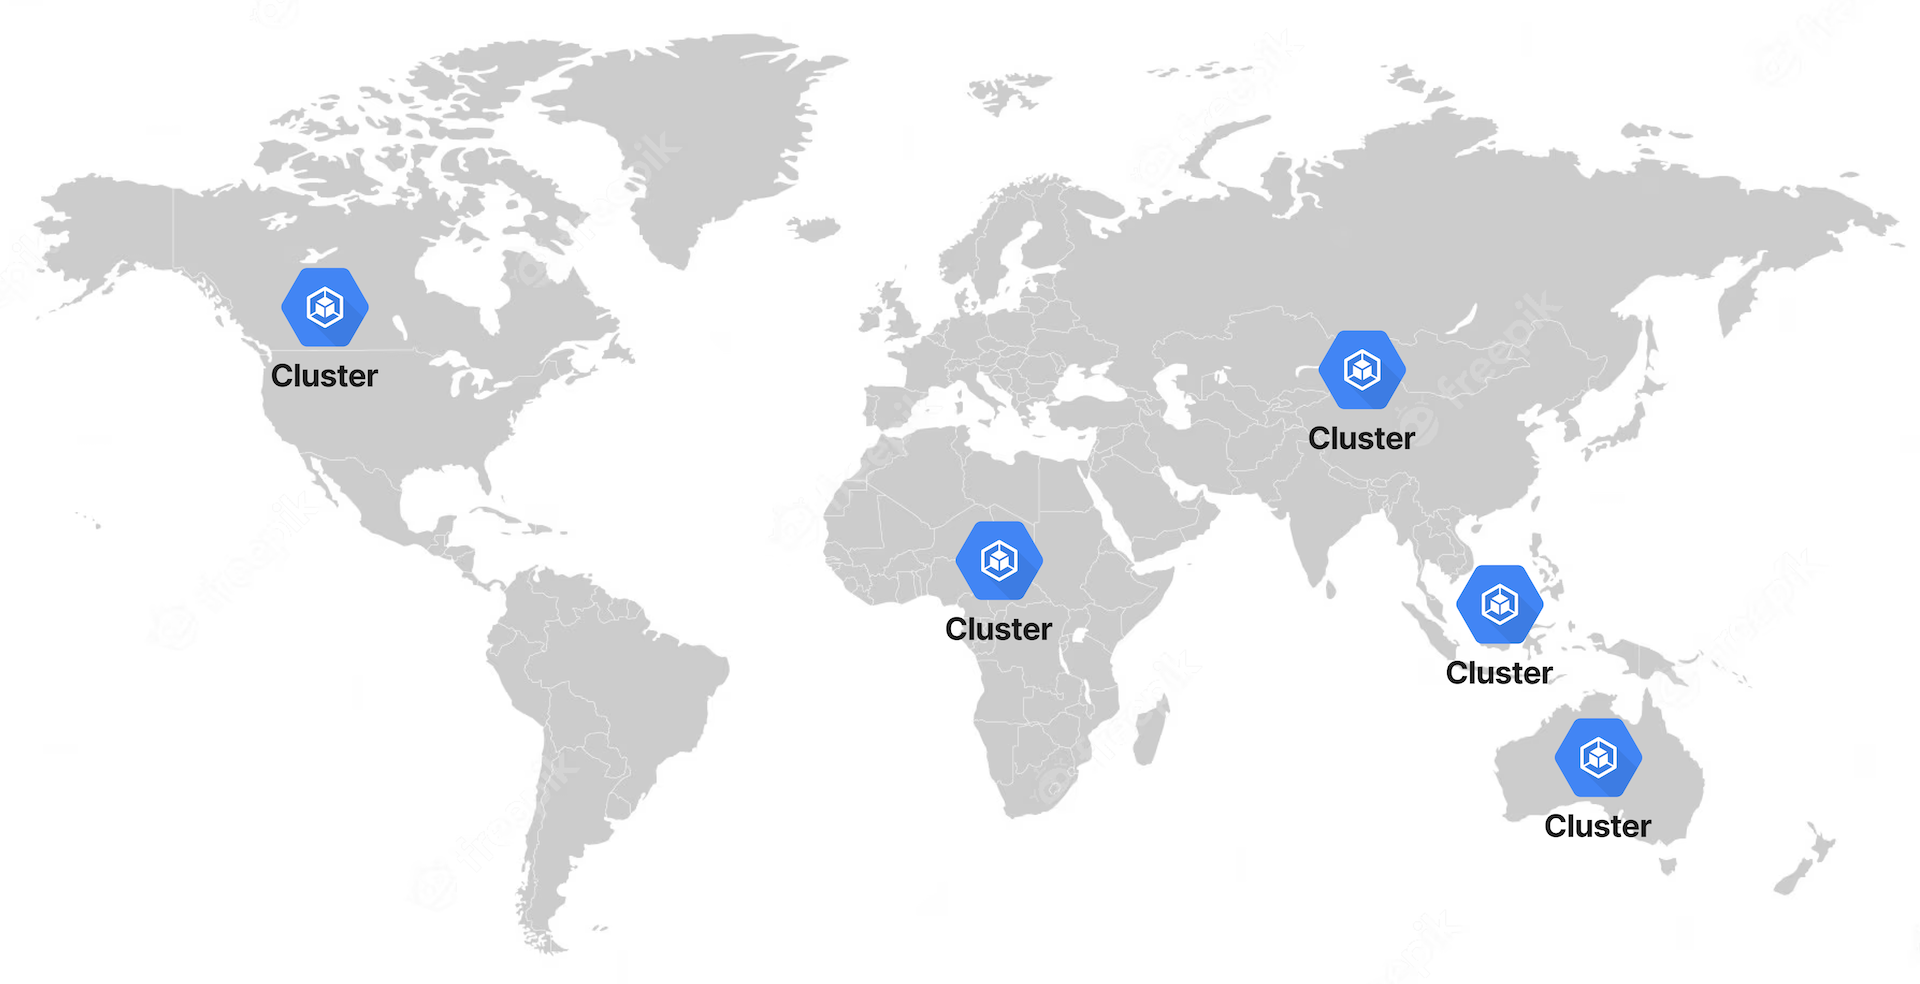
\includegraphics[width=1\textwidth]{assets/diagrams/geo-diagram.png}
	\caption{Geographically distributed clusters in different areas of the world.}
	\label{fig:geo-diagram}
\end{figure}

Geo-distributed clusters are multiple clusters hosted in different areas of the region. When an application's user base grows and spreads globally, a single central deployment may not offer the best user experience. The physical distance of a user to the server matters, which makes geo-distributed application deployment a good solution to accommodate users from all over the world. With the help of Kubernetes and a cloud provider, multi-regional deployment has never been easier. It is, however, a relatively new area in software development, and not much has been studied about the different approaches of this architecture. For this research, we have chosen two approaches: MultiClusterService with MultiClusterIngress and Istio / Anthos Service Mesh, as they are both are supported on the Google Cloud Platform.

In addition, geo-distributed clusters can be extended to databases, which can be seen in implementations such as CocroachDB. As different countries have different regulations, it is becoming a necessity for multinational companies to store user data in their respective region in order to comply with regulations. Data should be stored close to the users who access it most frequently and follow them when they travel to prevent high latencies caused by long-distance data retrieval \citep{taft-2020}. We used a simpler approach to achieve database geo-awareness, however, as geo-distributed databases introduce added complexities such as partition and replication, which are outside of this research scope.
% In addition, geo-distributed clusters can be extended to databases, which can be seen in implementations such as CocroachDB. The same benefits such as reduced latency can be gained in the data layer of an application, as different regulations between countries 


% Two geo-distributed clusters approaches studied in this research are MultiClusterService with MultiClusterIngress and Istio / Anthos Service Mesh.

\section{MultiClusterService (MCS) with MultiClusterIngress (MCI) (MCS with MCI}
To connect identical services across geo-distributed clusters, Fleet, MultiClusterIngresss, and MultiClusterService must be configured. A Fleet is a group of clusters that are visible to the MultiClusterIngress and can be used as backends. Inside a Fleet, a cluster needs to be designated as a config cluster where MultiClusterIngress and MultiClusterService are configured and deployed. Clusters that are registered to a Fleet besides the config cluster are called member clusters. 

MultiClusterService (MCS) is a custom GKE resource that allows services with the same selectors to be considered the same by creating derived services in the member clusters. The derived service creates a Network Endpoint Group (NEG) in every target cluster which tracks pod endpoints and allows service discovery, as shown in \autoref{fig:mcs-derivation}. MCS integrates with Google's Fleet to define target clusters to create derived service resources. By default, every cluster registered to a Fleet is considered a target cluster.

MultiClusterIngress (MCI) is a custom resource that sends traffic to the default backend MCS or based on rules configured to route hosts to a certain backend MCS and creates a layer 7 Virtual IP (VIP) address that routes traffic to backends that are configured in multiple clusters as MCS and can be accessed by public users. MultiClusterService and MultiClusterIngress are configured identically to their non-multi counterpart and are only deployed in the config cluster.

\begin{figure}
	\centering
	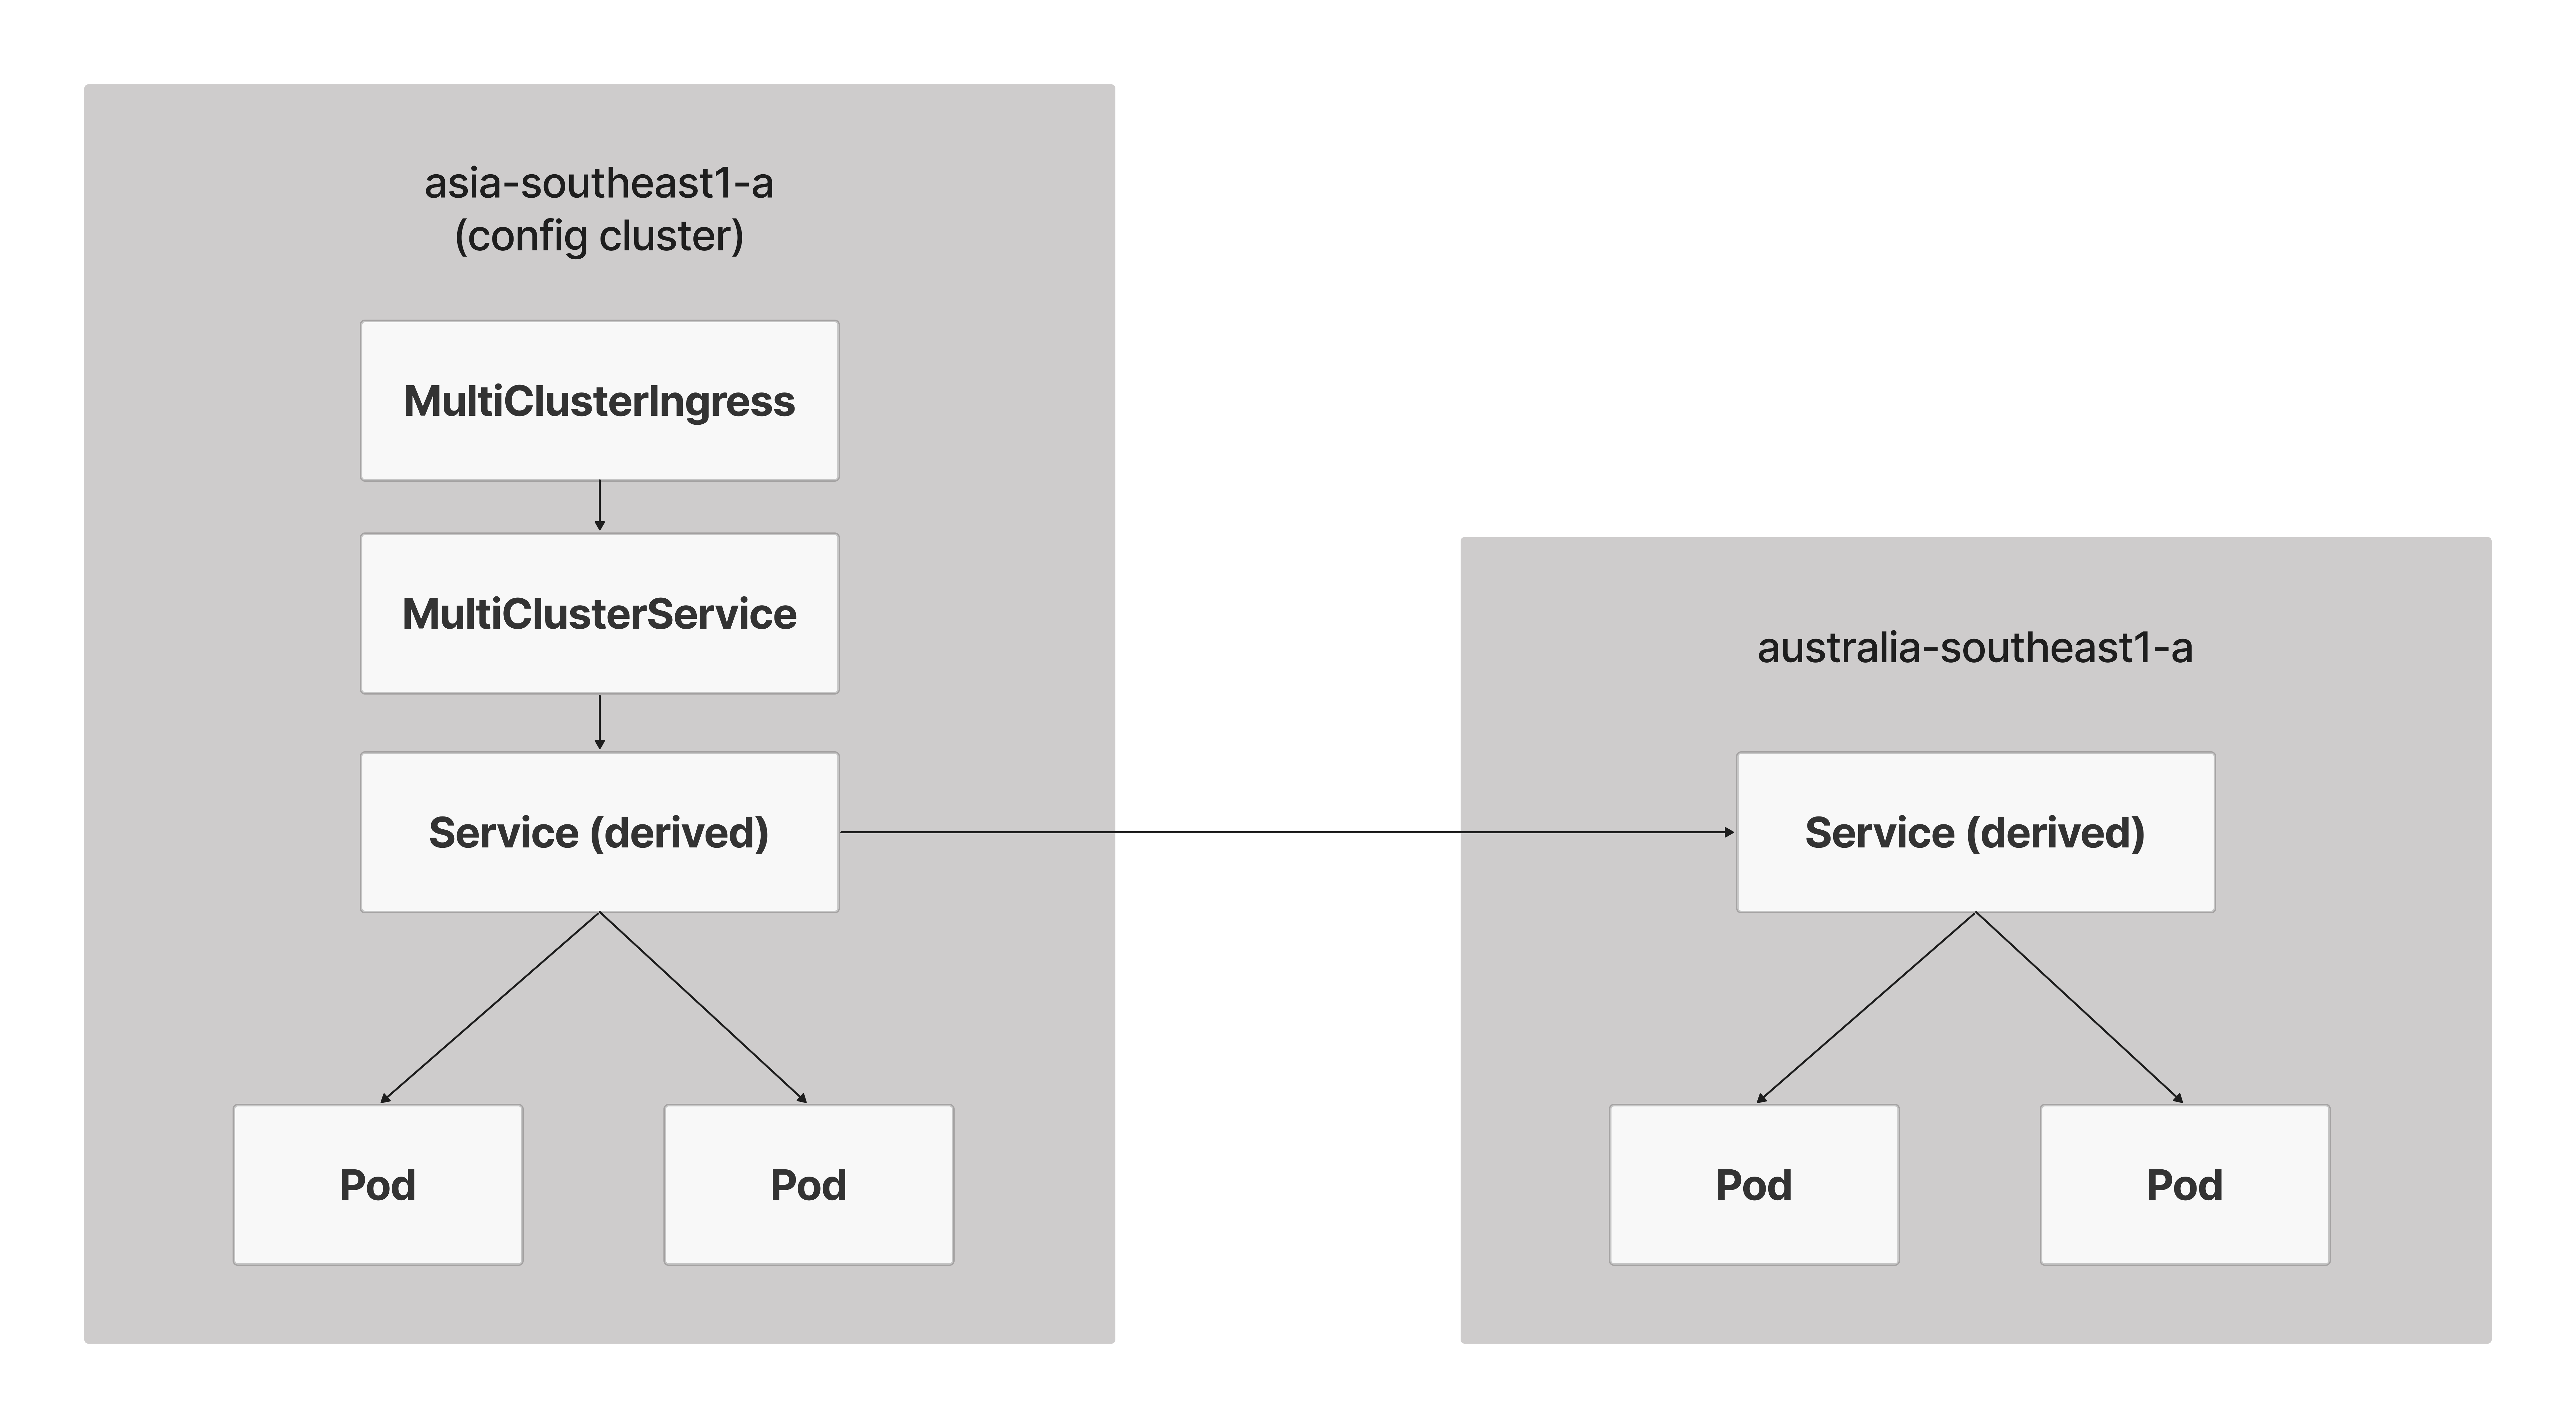
\includegraphics[width=1\textwidth]{assets/diagrams/mcs-mci.png}
	\caption{Service derivation using MultiClusterIngress and MultiClusterService.}
	\label{fig:mcs-derivation}
\end{figure}

% \section{Google Cloud Load Balancer}
% \label{sec:cloudLoadBalancer}
In a multi-cluster GKE setup using MCS with MCI, MCI deploys load balancers across clusters registered to a Fleet. The type of load balancer deployed by an MCI is a global external load balancer and is categorized as north-south routing, meaning that it routes traffic from outside to inside of the data center, as seen in \autoref{fig:gclb-diagram}.

\begin{figure}
	\centering
	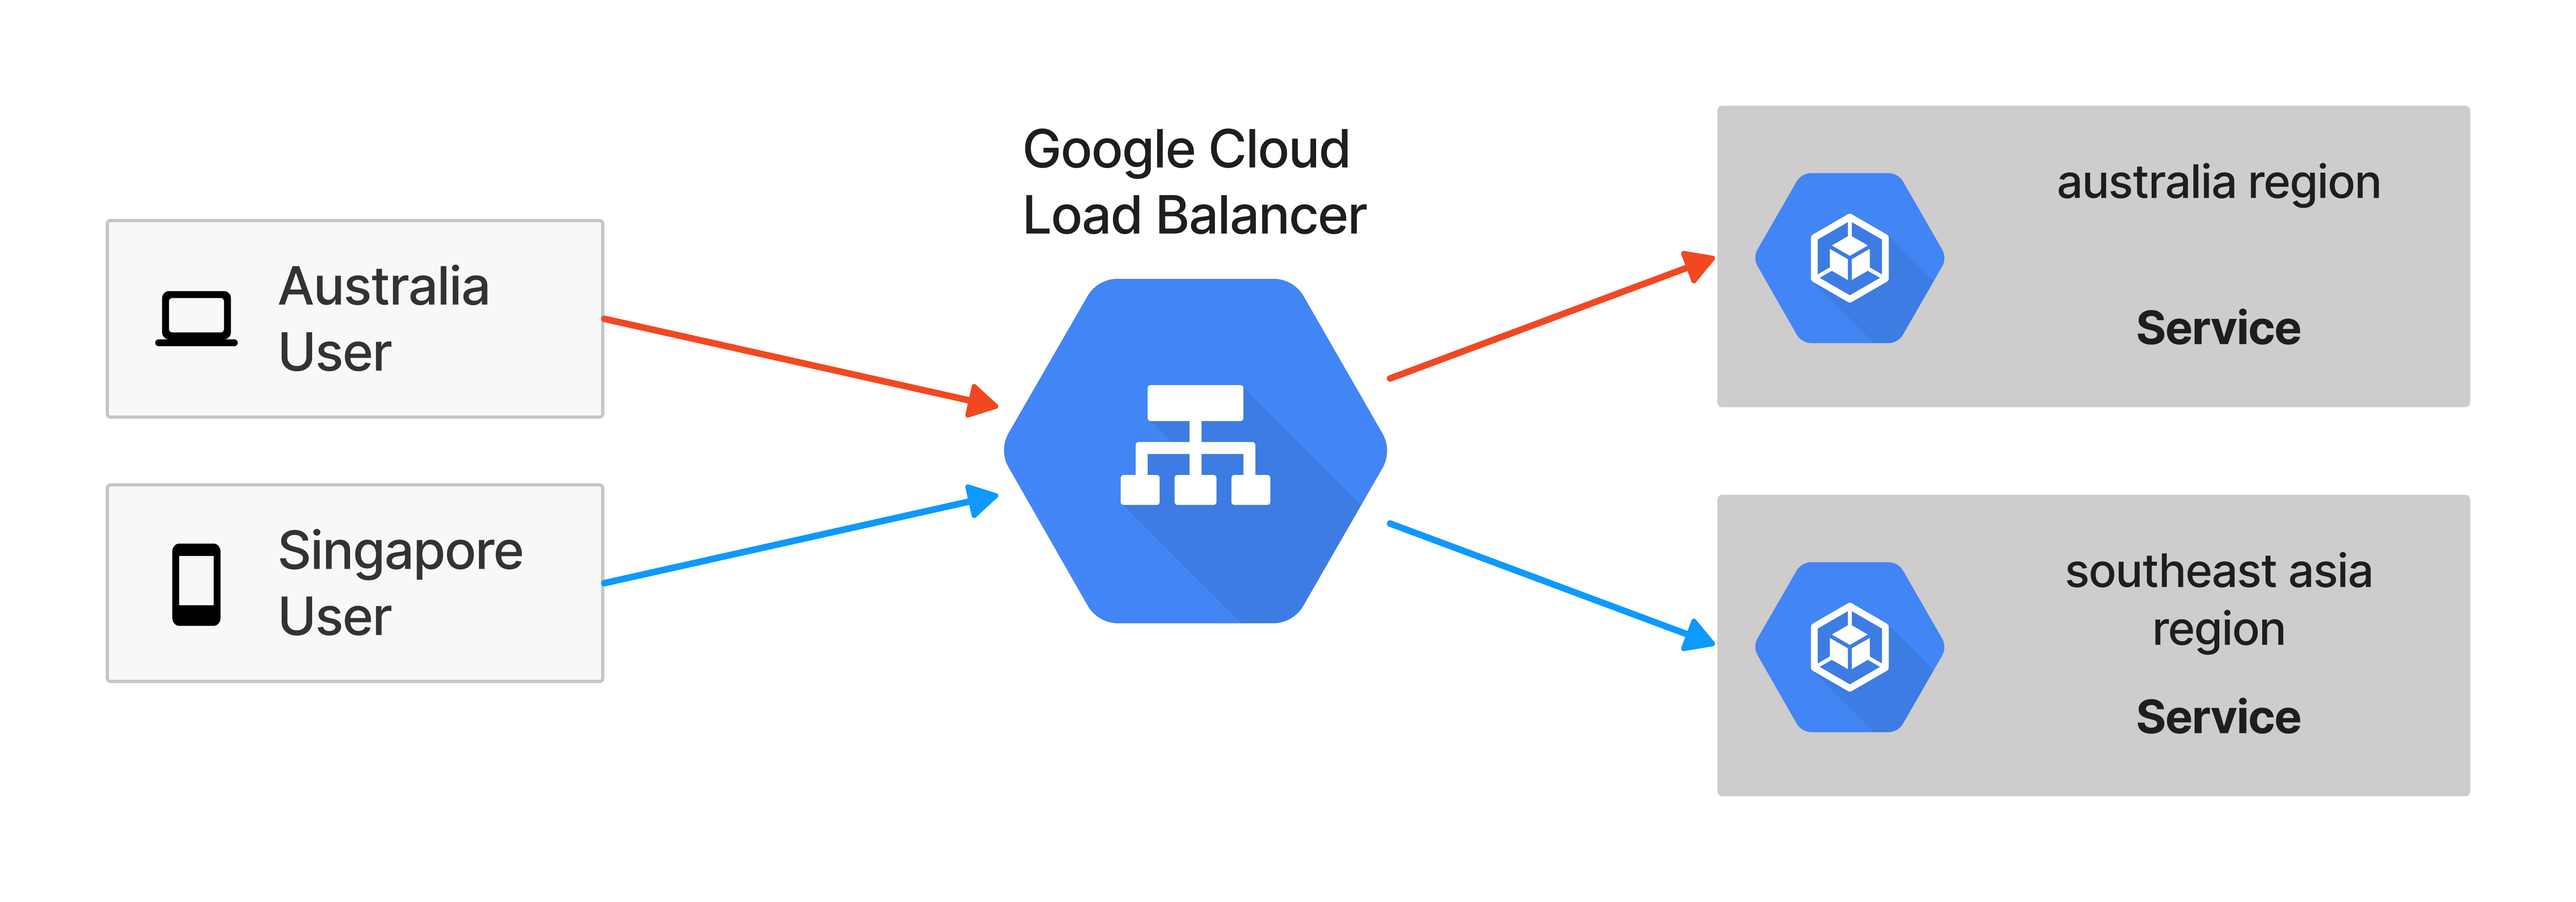
\includegraphics[width=1\textwidth]{assets/diagrams/gclb-diagram.png}
	\caption{Google Cloud Load Balancer traffic routing.}
	\label{fig:gclb-diagram}
\end{figure}

The global external load balancer routes traffic to the closest Google Point of Presence (PoP) and uses a single anycast IP address deployed to multiple regions \citep{google-mci-2023}. There is also a premium network tier that offers cold-potato routing to Google PoPs and hot-potato routing inside Google networks.
% Google Cloud Load Balancer uses a single Anycast IP which routes users to the closest Google Point of Presence (PoP).

\section{Istio / Anthos Service Mesh}
\label{sec:istio}
The other option for multi-cluster Kubernetes deployment presented in this research is using Istio / Anthos Service Mesh. Istio is an open-sourced service mesh platform that is used to connect microservices and adds features such as observability, security, and traffic management. Istio on GKE is not supported since September 2022 but users can still use Istio under the name of Anthos Service Mesh on the Google Cloud Platform. Anthos Service Mesh (ASM) is compatible with Istio custom resources. ASM has the benefit of a managed control plane that handles automatic upgrades as well as a managed data plane that automatically upgrades sidecar proxies and injected gateways by evicting old pods that are running a prior version \citep{google-asm-2023}. Automatic sidecar injection is the core of Istio's functionality, allowing pods to be injected with the Envoy proxy at creation, as shown in \autoref{fig:envoy-proxy-injection}. Envoy proxy mediates all inbound and outbound traffic for all services in a service mesh. For a multi-cluster Anthos Service Mesh, ASM integrates with the Fleet API just like the MCS with MCI approach, but there is no config cluster. Instead, installing ASM on every cluster is needed to register them to the service mesh.

\begin{figure}
	\centering
	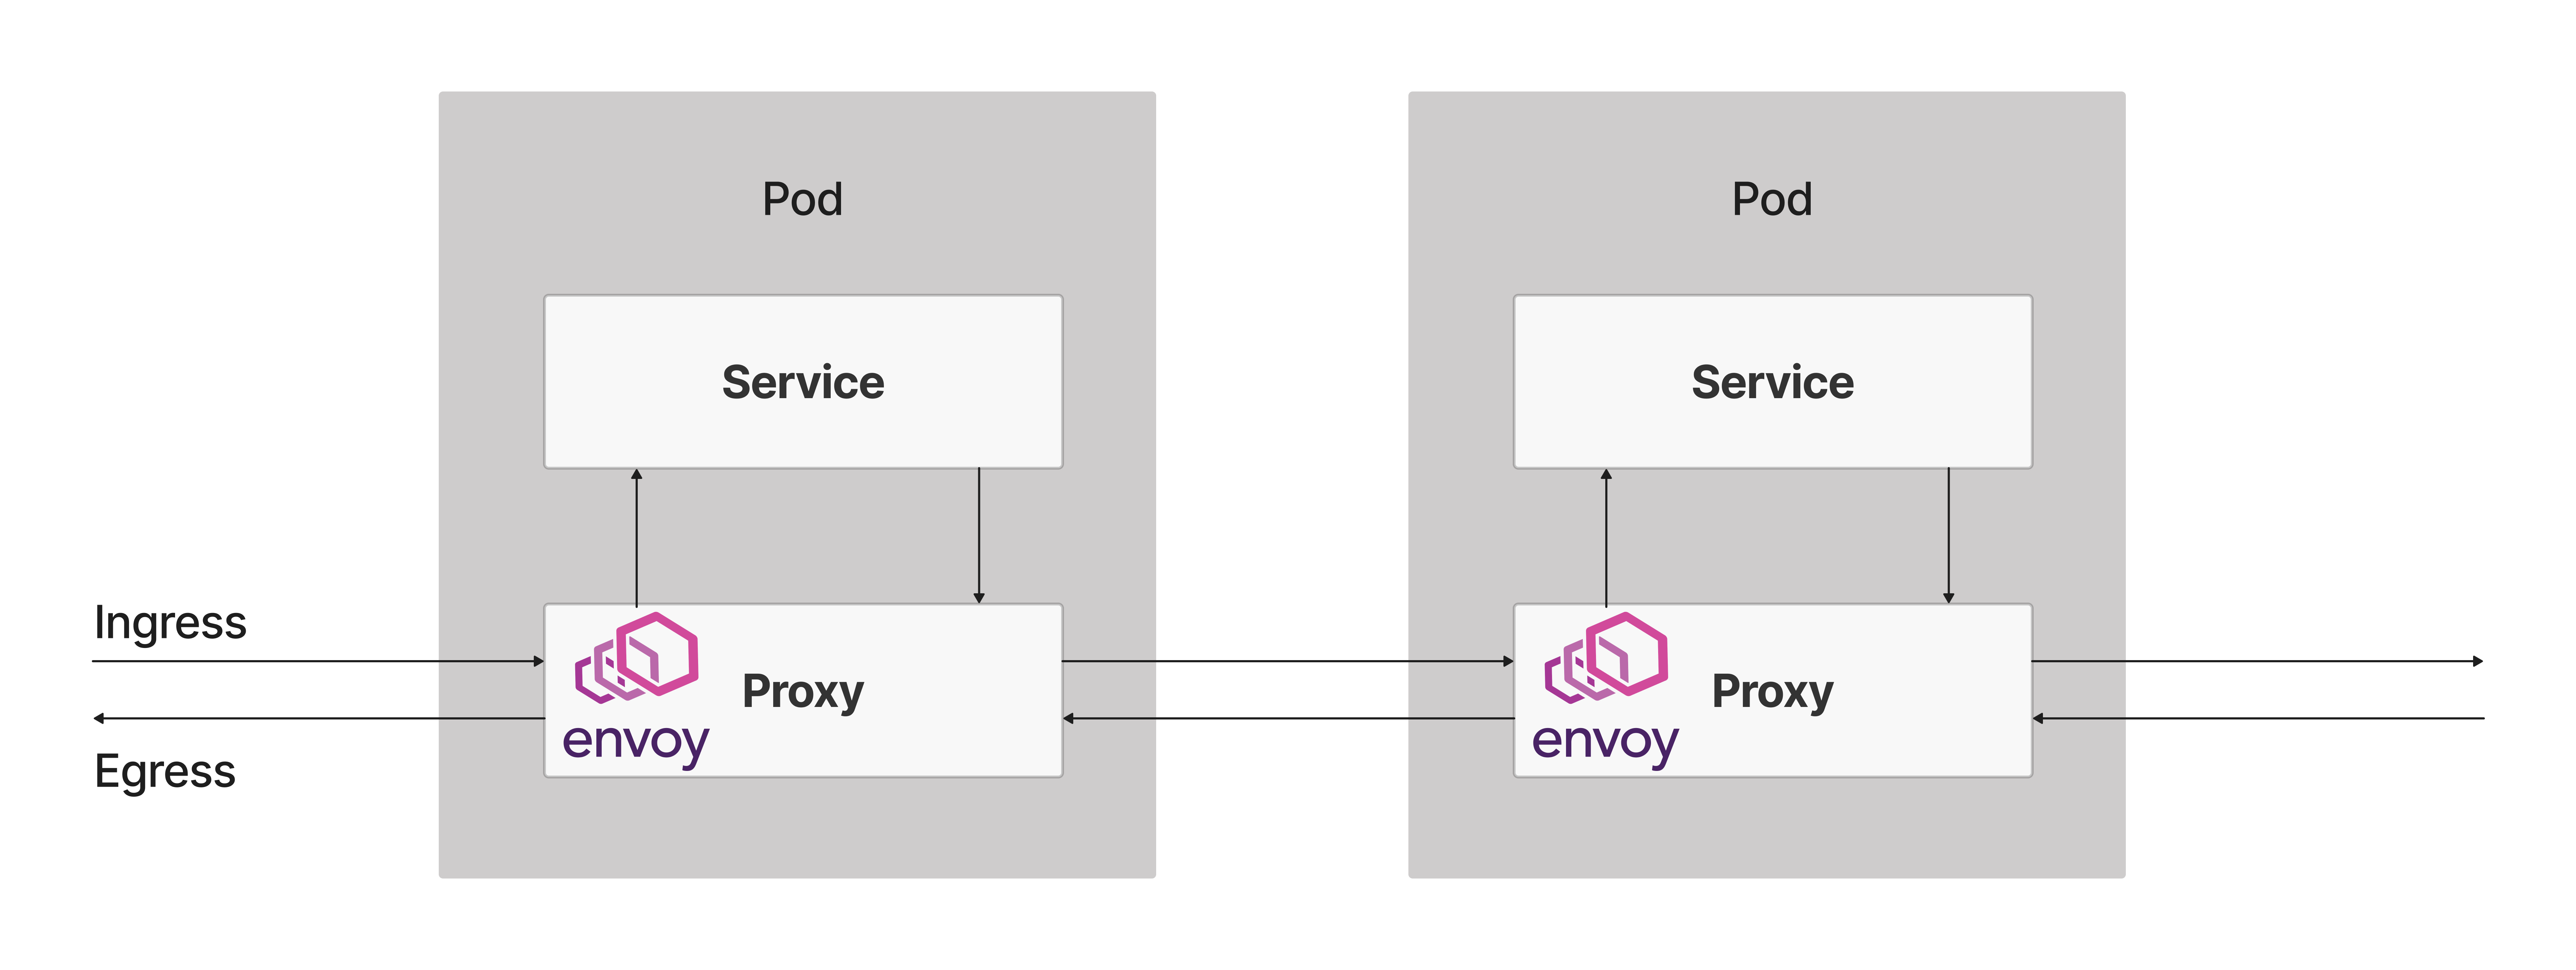
\includegraphics[width=1\textwidth]{assets/diagrams/envoy-proxy.png}
	\caption{Envoy proxy injection and interaction with service inside of a pod.}
	\label{fig:envoy-proxy-injection}
\end{figure}

% \subsection{Locality Load Balancing}
The default load balancer algorithm for Istio is round-robin, where traffic is distributed to clusters in a circular way such that each cluster will be chosen once in a cycle. One of the benefits of this approach is that it prevents an instance where a single server is overloaded by requests by distributing traffic equally to all servers. An approach to reduce latency by closing the physical gap between user and server, locality load balancing is proposed as a better solution for an application with geo-distributed clusters. Locality load balancing is a feature of Istio from using another open-sourced application called Envoy. Locality load balancing, also known as geographical load balancing, is a location-aware load balancer that can efficiently route traffic to the nearest cluster available and can be seen in \autoref{fig:locality-lb-diagram}. To enable locality load balancing, a DestinationRule resource must be configured. DestinationRule defines rules that apply to traffic for a service. DestinationRule can be configured to enable load balancing and outlier detection which work together to determine healthy hosts that are able to handle the traffic.

\begin{figure}
	\centering
	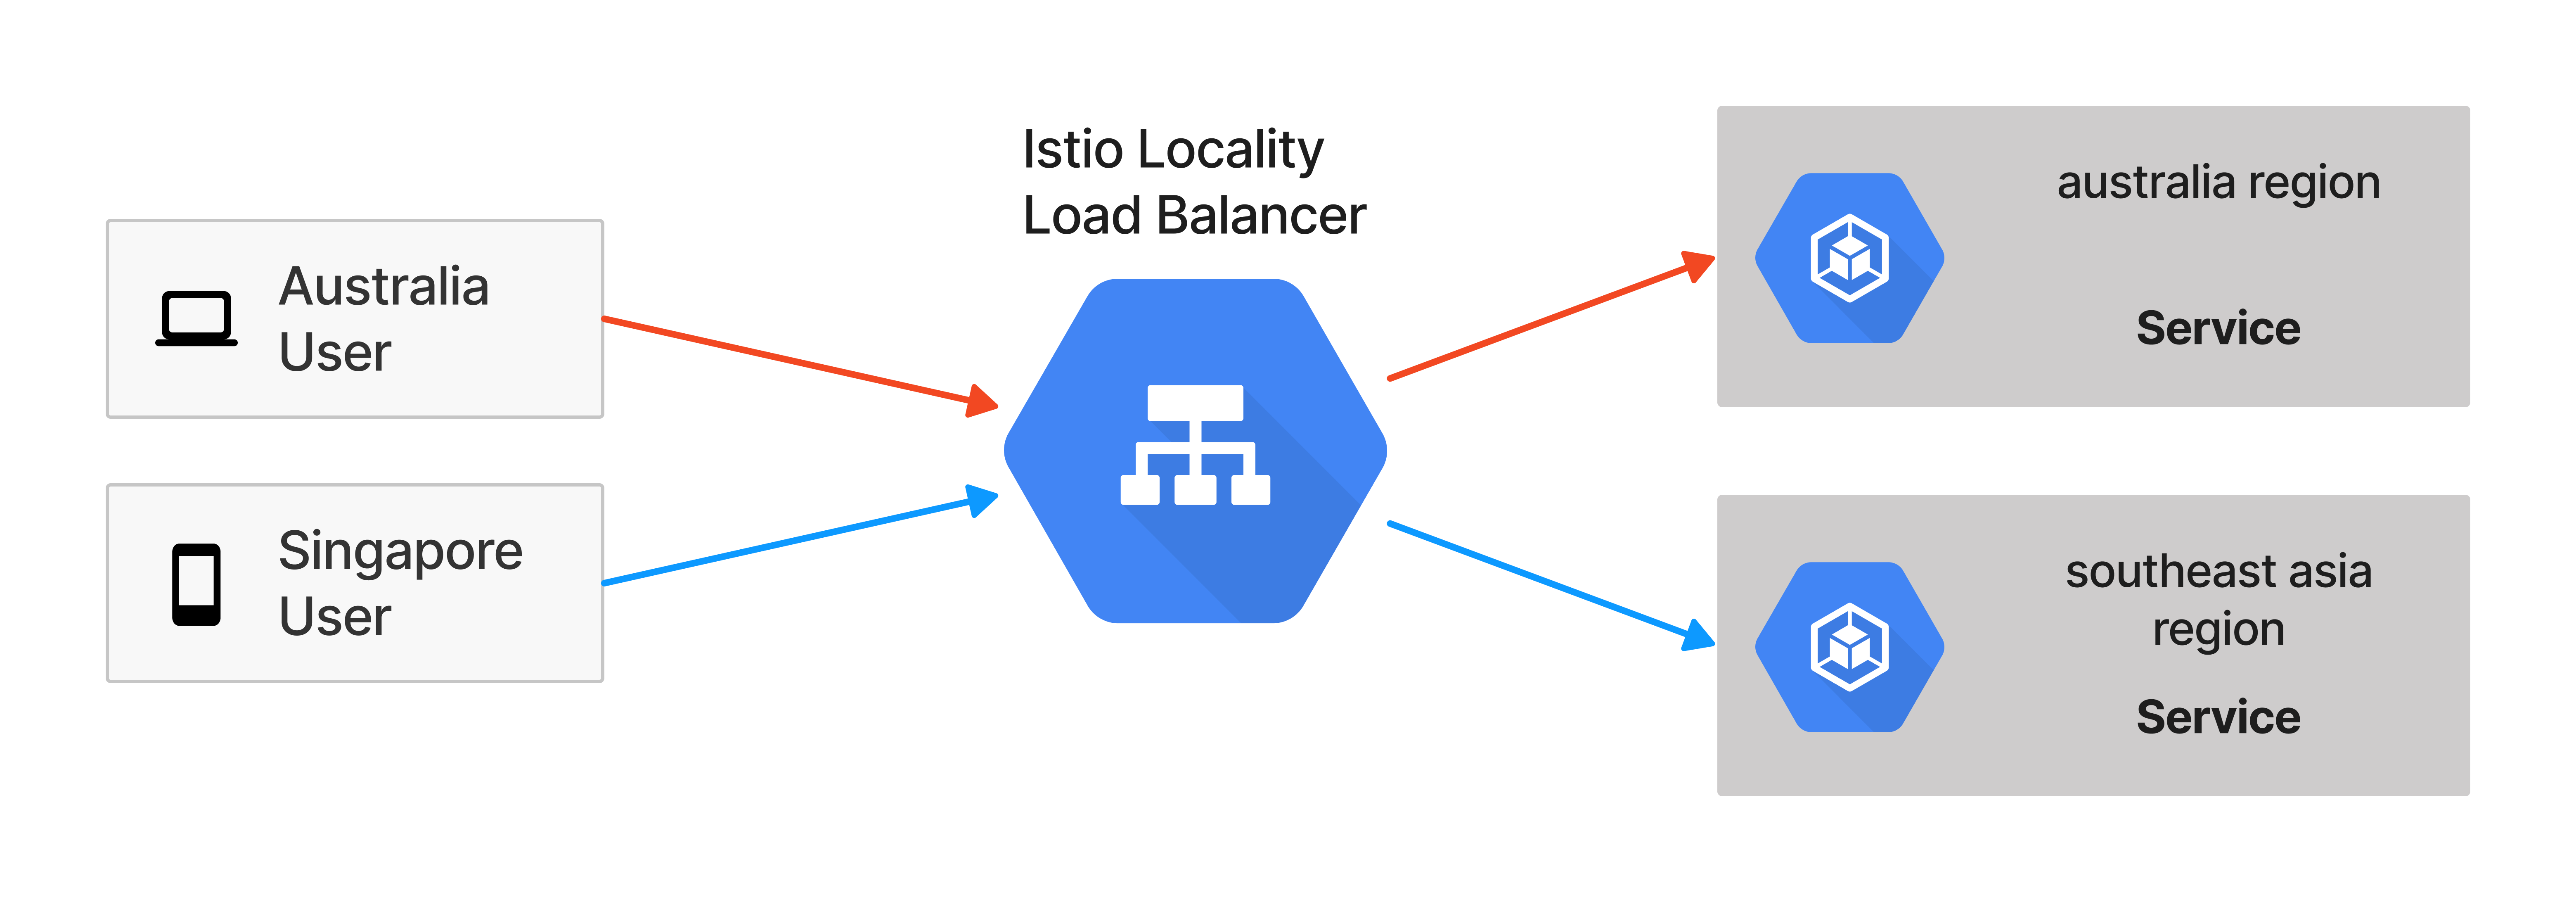
\includegraphics[width=1\textwidth]{assets/diagrams/locality-lb-diagram.png}
	\caption{Istio Locality Load Balancer traffic routing.}
	\label{fig:locality-lb-diagram}
\end{figure}

The main difference between these two methods is their architecture. Istio / ASM introduces an additional layer of complexity, built on top of the Kubernetes architecture to add functionalities that utilize Istio's proxy injection on each pod. Meanwhile, the MCS with MCI approach is an extension of the Kubernetes API, where additional resources such as MultiClusterService and MultiClusterIngress are used to take advantage of Google Cloud's multi-region servers. In addition, MCS with MCI only has a fraction of features compared to Istio / ASM, as it is intended to be used in conjunction with other Google services such as the Google Cloud Load Balancer.

% When we create an Istio ingress, a public IP address is reversed for the dedicated LoadBalancer \citep{xie-2020}.

\section{Performance}
Performance is an important part of web applications and can be measured using different evaluation metrics. The metrics that can measure an application's performance are latency, requests per second, and success rate. Latency is the amount of time it takes for a server to respond to complete a user's request. Lower latency is better, as it results in more requests that are able to be handled and reduces the load of a server. Most importantly, lower latency creates a better user experience as it minimizes the time a user needs to wait while using an application. Latency itself doesn't paint the full picture of application performance, requests per second (RPS) can help measure an application's ability to handle multiple users simultaneously and is a measurement of how many requests an application can handle in a period of time. During peak hours when the application traffic is at its highest, having a high RPS reduces the occurrence of a server bottleneck.

Furthermore, another important metric for a web application to have is reliability. A web service's reliability is the likelihood of a server finishing a request under certain time and workload conditions  \citep{bhalerao-2019}. Measuring a server's reliability is useful to determine how well a server can handle certain real-world scenarios such as high-traffic hours, where a website can expect a heightened number of requests. Without application reliability, businesses that rely on web applications could potentially lose a significant amount of revenue as users aren't able to complete their transactions due to their servers not being able to respond to the client's requests. To measure the percentage of requests being processed as intended, success rate is a metric to quantify just that. Success rate is a measure of how often an application successfully responds to the user's request. A failure can occur when a user inputs something unintended or when a server is unable to process a request caused by the server being overloaded and is indicated by a response code outside of [200, 400], inclusive. The latter definition is used when referring to a failed response as requests are validated and standardized in testing scenarios. 
% It is important for a web application to be reliable, as it could 

To measure the effectiveness of each multi-cluster scenario, performance testing such as load testing and stress testing is done to simulate scenarios where an application receives various amounts of traffic with the possibility of server failure. Load testing is done to measure the performance of a web application at a certain load level to ensure that the website can be worked within the range of multi-user concurrency requirements \citep{yu-2019}. Load testing is also done to identify a server's maximum performance capability by evaluating performance metrics on every increase in load level. On the other hand, stress testing is done to analyze the web application's ability to do failure recovery, which happens after a server is forced to restart due to a server failure. Stress testing can identify a machine's readiness to adopt certain changes that consume resources, such as a service mesh. Performance testing and evaluation metrics are crucial to determine the performance of each approach for geo-distributed clusters.


% \begin{itemize}
%     \item Latency \\
%     Latency is the amount of time it takes for a server to respond to complete a user's request. Lower latency is better, as it results in more requests that are able to be handled and reduces the load of a server. Most importantly, lower latency creates a better user experience as it minimizes the amount of time a user needs to wait while using an application.
%     \item Requests per second \\
%     Requests per second (RPS) is a measurement of how many requests an application can handle in a second. RPS can measure an application's ability to handle multiple users simultaneously. During peak hours when the application traffic is at its highest, having a high RPS reduces the occurrence of a server bottleneck.
%     % \item Survivability \\
%     % Survivability is a measu
%     \item Success rate \\
%     The success rate measures how often an application successfully responds to the user's request. A failure can occur when a user inputs something unintended or when a server is unable to process a request caused by the server being overloaded and is indicated by a 5xx response code. The latter definition is used when referring to a failed response as requests are validated and standardized in testing scenarios. 
% \end{itemize}

\clearchapter
%-----------------------------------------------------------------------------%
\chapter{\babTiga}
\label{bab:3}
%-----------------------------------------------------------------------------%
This chapter explains the methodology used in this research. The discussion in this chapter includes research stages, application infrastructure design, testing scenarios, and evaluation metrics.

\section{Research Stages}
\label{sec:researchStages}
There are several stages in this research, which include problem formulation, literature study, application design and implementation, performance evaluation and analysis, and inference. The entirety of the research stages can be seen in \autoref{fig:research-stages}
%-----------------------------------------------------------------------------%
\begin{figure}
	\centering
	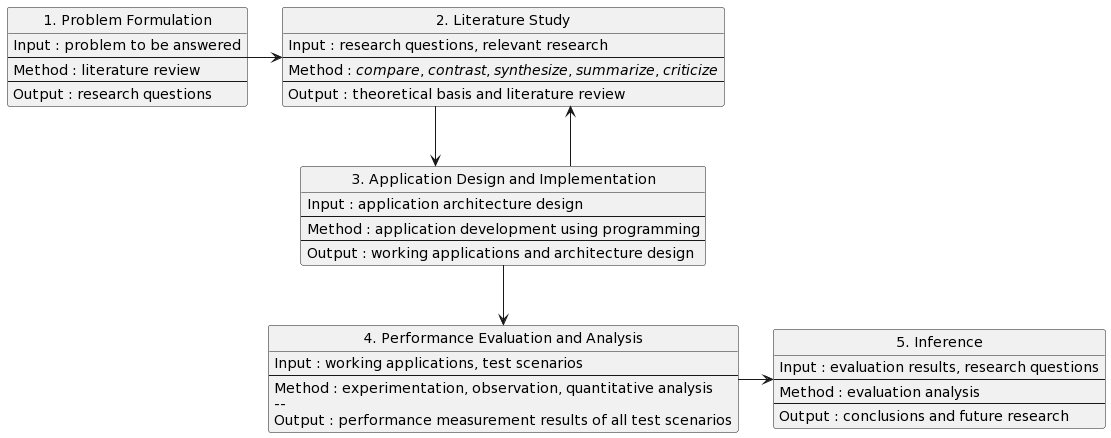
\includegraphics[width=1\textwidth]{assets/diagrams/research-stages.png}
	\caption{Research stages.}
	\label{fig:research-stages}
\end{figure}

In the first stage, problem formulation, existing problems are used with the help of literature review to produce research questions that are answered in the conclusion of this study. In the second stage, literature study, relevant research is used to define/create the basis of this research. The methods used in the literature study stage are the following: compare, contrast, synthesize, summarize, and criticize which helps to get the theoretical foundation and literature review of this research.

In the third stage, application design and implementation, the web application architecture is designed and implemented to be used as a common variable for testing to be done. The configuration of geo-distributed Kubernetes clusters and Istio service mesh is also done in this stage. In the fourth and penultimate stage, testing is done, and each testing scenario is evaluated to answer research questions and acquire a conclusion for this study, which is done in the final stage.

% \section{Application Infrastucture Design}
% \label{sec:applicationInfrastructureDesign}
% Two areas that need to be configured in the complete web application are the application server itself and the geo-distributed Kubernetes clusters. The application is a two-tiered application consisting of a server and database tier. The client tier is omitted from the application itself but instead is represented by the Vegeta load testing tool. The server is a REST API that communicates with a database and simply returns the cluster name of where the responding server is located. The server is then containerized using Docker and uploaded to Docker Hub to be used by Kubernetes. This separation of concern between application development and infrastructure development allows for concurrent progress to be made between the two different areas and is a big reason why Docker and Kubernetes are widely adopted.

% The next step after application configuration is the geo-distributed clusters configuration. The two different configurations are MCS with MCI and Istio / ASM. For the MCS with MCI configuration, the server service is deployed as a MultiClusterService custom resource and is routed by the MultiClusterIngress custom resource which allows cross-cluster communication. A virtual IP address is then created which uses a Google Cloud Load Balancer that routes traffic to the nearest cluster. The infrastructure for the MCS with MCI geo-distributed Kubernetes clusters can be seen in \autoref{fig:infra-mcs-mci}.

% \begin{figure}
% 	\centering
% 	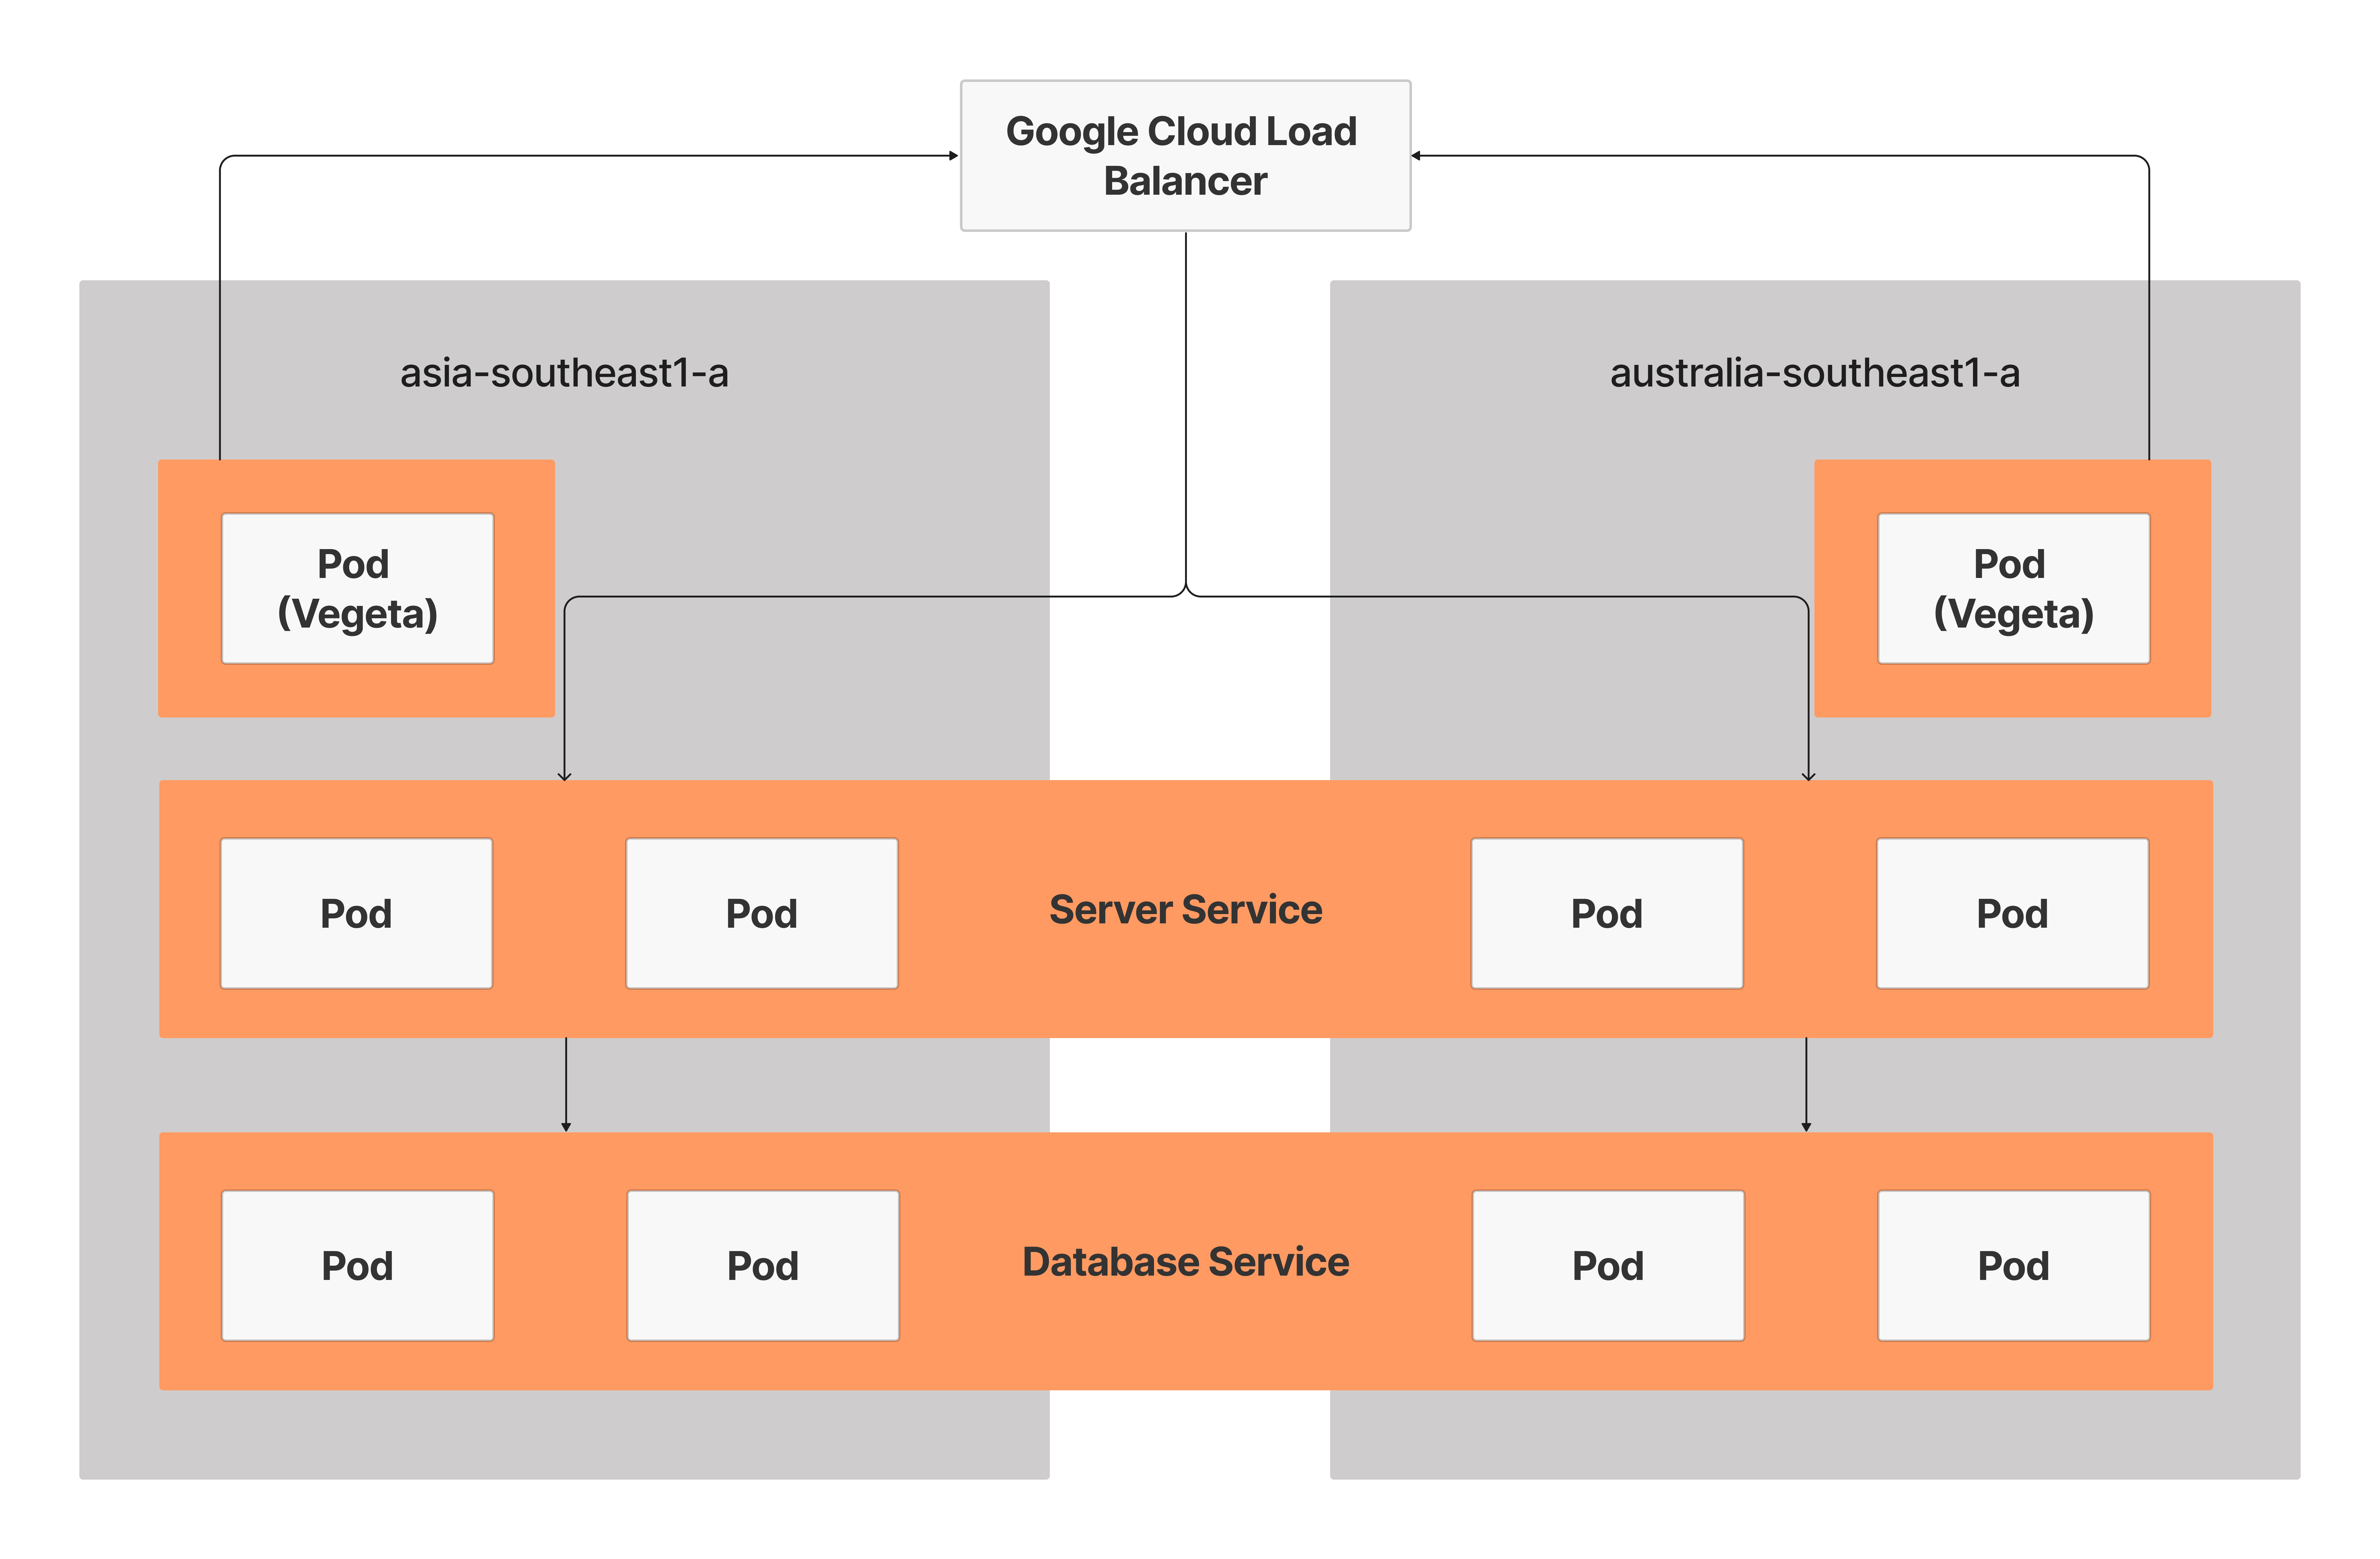
\includegraphics[width=1\textwidth]{assets/diagrams/infra-mcs-mci.png}
% 	\caption{Geo-distributed Kubernetes clusters infrastructure on the MCS with MCI configuration.}
% 	\label{fig:infra-mcs-mci}
% \end{figure}

% For the Istio / ASM configuration, each cluster is installed with Istio control and data plane which enables automatic envoy proxy injection to each pod. A DestinationRule resource is then deployed to configure locality load balancing which routes traffic to the nearest cluster. The Vegeta load testing pod is deployed in every region to simulate a request call from each region. The database layer can't be load balanced directly, as a database instance is needed on the server runtime. An approach to counter this is to have a dedicated data layer which is a server for each database instance. The infrastructure for the Istio / ASM geo-distributed Kubernetes clusters can be seen in \autoref{fig:infra-istio}.

% \begin{figure}
% 	\centering
% 	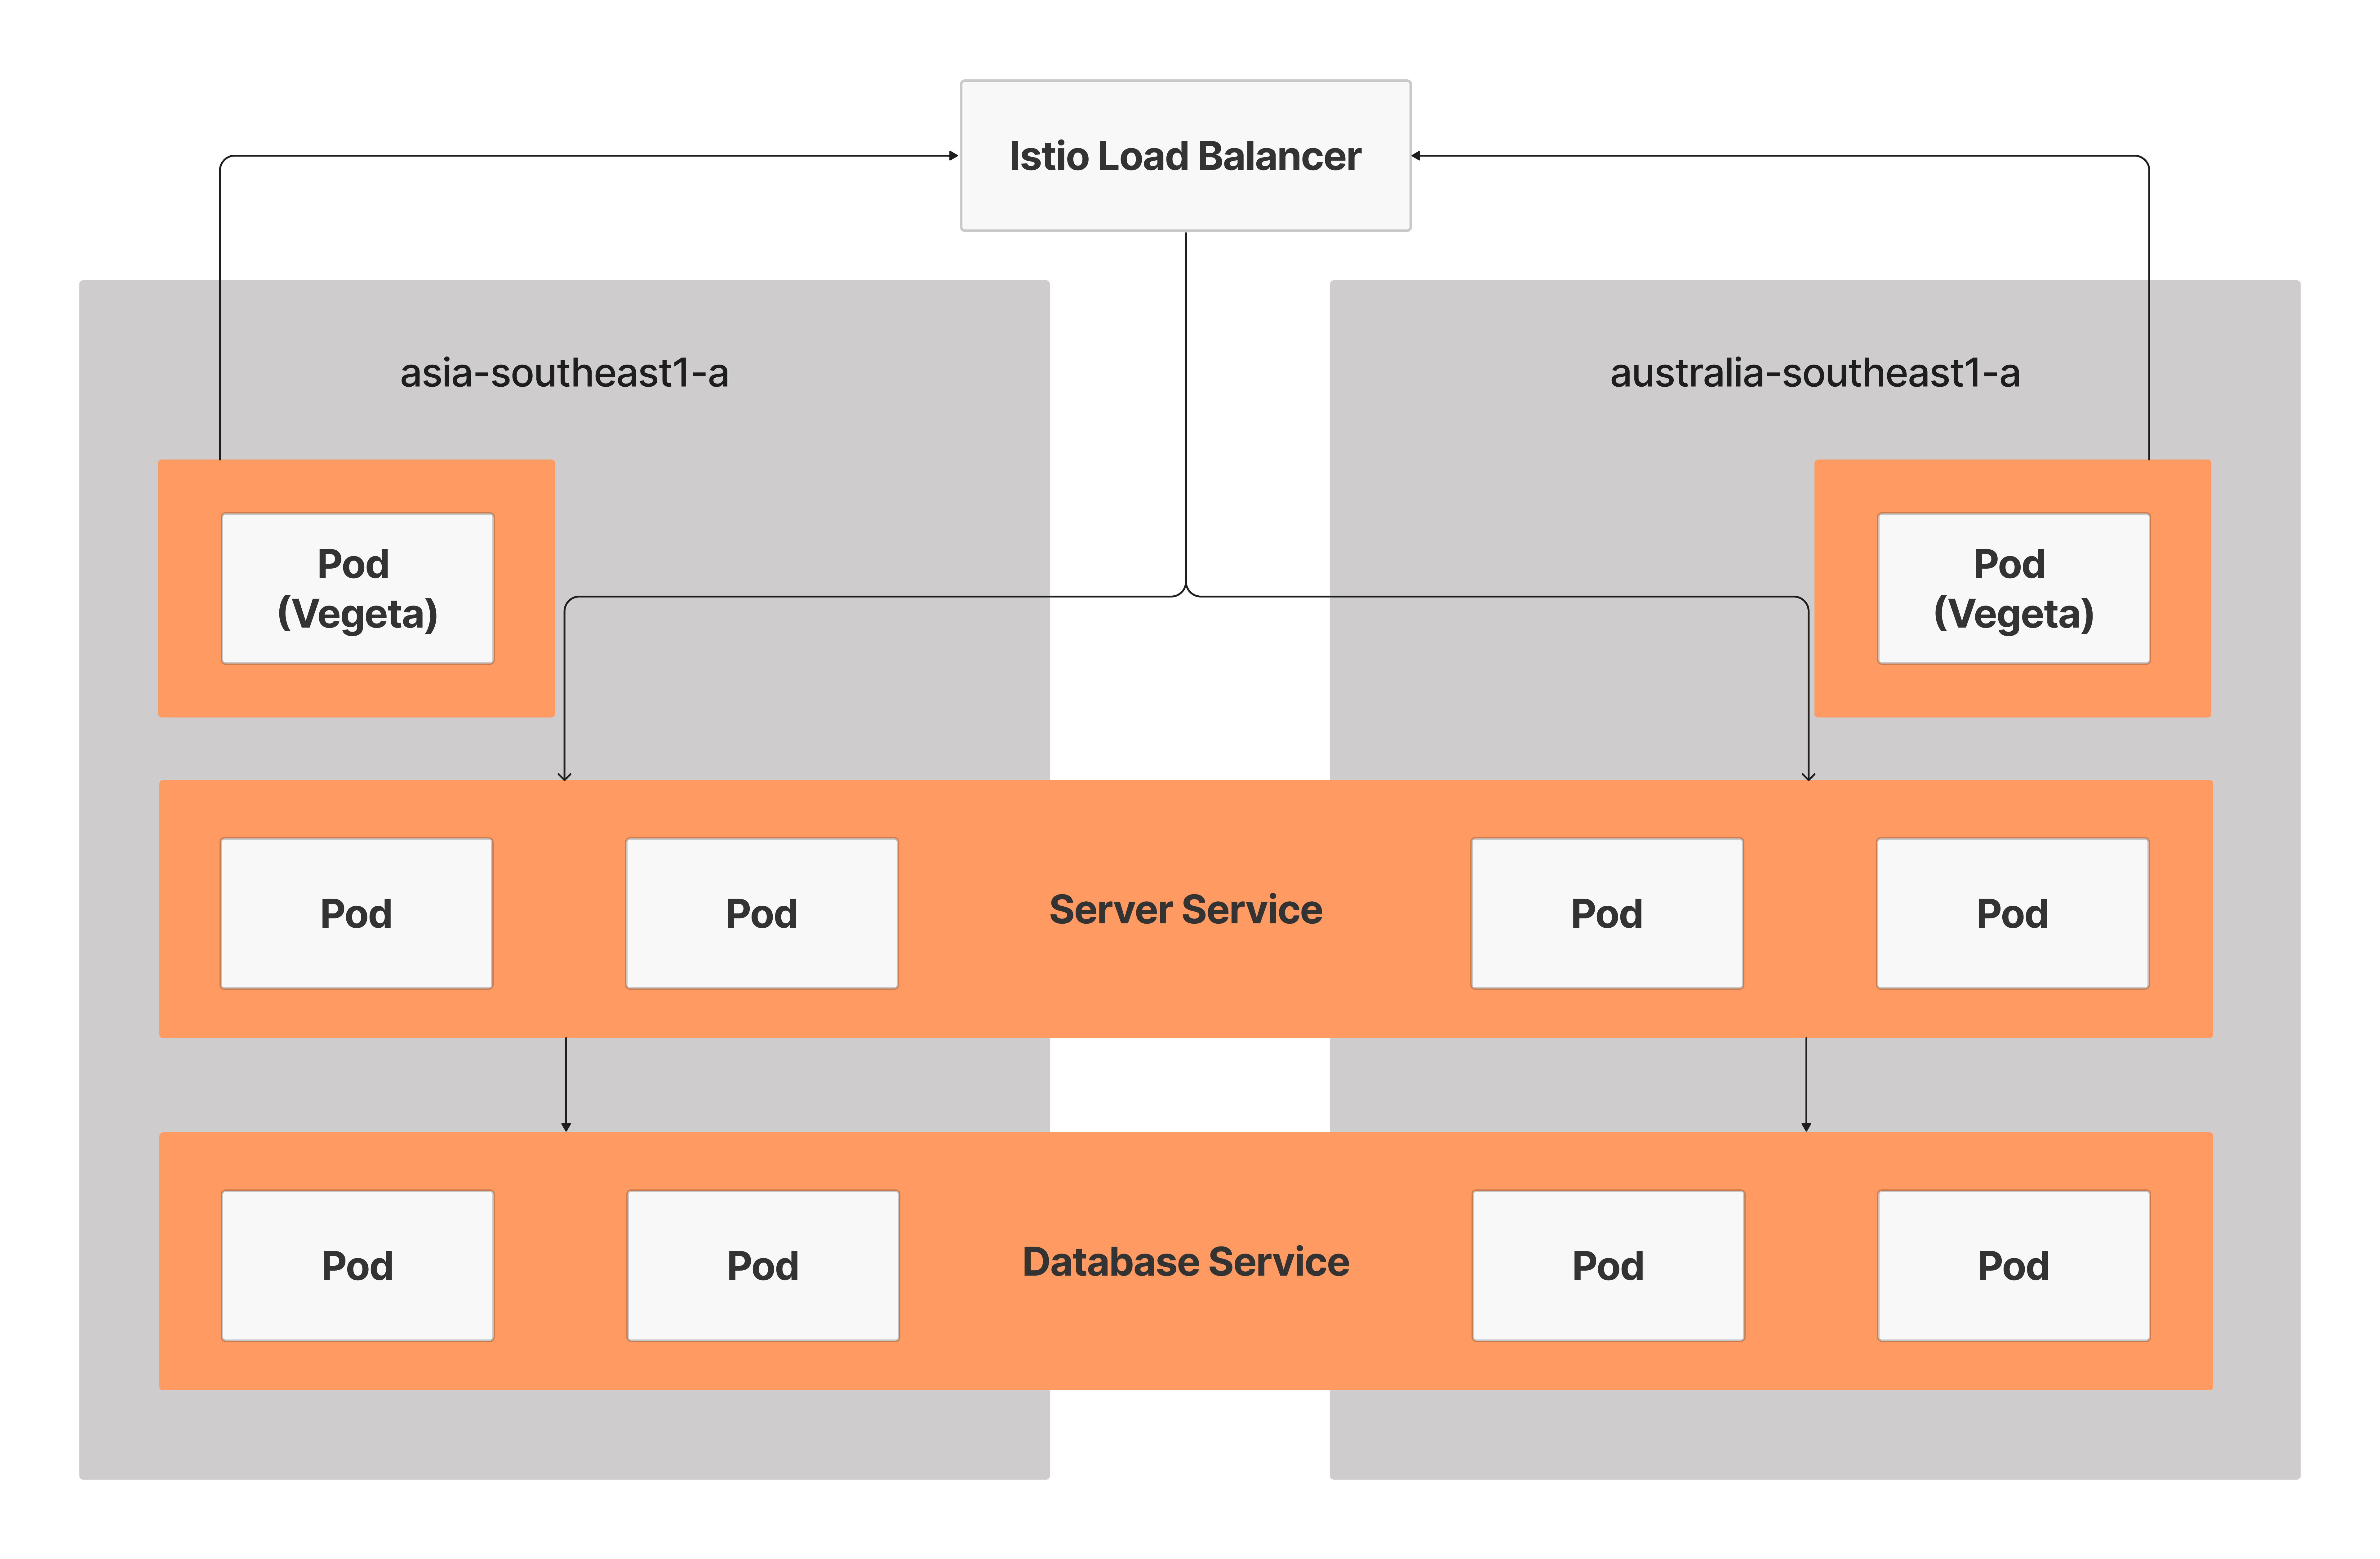
\includegraphics[width=1\textwidth]{assets/diagrams/infra-istio.png}
% 	\caption{Geo-distributed Kubernetes cluster infrastructure on Istio / ASM configuration.}
% 	\label{fig:infra-istio}
% \end{figure}

\section{Testing Scenarios}
\label{sec:testingScenarios}
In the testing scenario, load testing and stress testing are done to evaluate the performance of each geo-distributed cluster configuration. Being a quantitative research and quantitative experimentation, there are variables that need to be established. The independent variables are the different geo-distributed Kubernetes cluster configurations, load balancer algorithm, and the different requests per second configured during performance testing. For each geo-distributed cluster configuration, testing is done by increasing the RPS after each test case. Each test case occurs for 5 seconds to simulate a short period where a server experiences high traffic, for example during a flash sale. The RPS used in the testing configuration are 10, 50, and 100 where 100 is the upper limit chosen from the number of errors that occurred during preliminary tests. The independent variables are shown in \autoref{table:combined-config}.

% \begin{table}
% \centering
% \begin{tabular}{|c|c|}
% \hline
% Geo-Distributed Cluster Configuration                      & Load Balancer \\ \hline
% MCS with MCI                    & Geo-Aware                    \\ \hline
% Istio / ASM                 & Round Robin                              \\ \hline
% Istio / ASM                  & Geo-Aware                   \\ \hline
% \end{tabular}
% \caption{Configuration of geo-distributed clusters}
% \label{table:geo-distributed-cluster-test-config}
% \end{table}

% \begin{table}
% \centering
% \begin{tabular}{|c|}
% \hline
% Region Request Origin Configuration                      \\ \hline
% asia-southeast1-a \\ \hline
% australia-southeast1-a \\ \hline
% \end{tabular}
% \caption{Configuration of region request origin}
% \label{table:region-origin-test-config}
% \end{table}

% \begin{table}
% \centering
% \begin{tabular}{|c|}
% \hline
% Requests Per Second (RPS) Configuration                       \\ \hline
% 10                                        \\ \hline
% 50                                               \\ \hline
% 100                                    \\ \hline
% \end{tabular}
% \caption{Configuration of requests per second (RPS)}
% \label{table:rps-test-config}
% \end{table}

% \begin{table}[htbp]
\begin{table}
\centering
\caption{Configuration of geo-distributed cluster method, load balancer, and requests per second}
\begin{tabular}{|c|c|c|}
\hline
Geo-Distributed Cluster Method & Load Balancer & Requests Per Second (RPS) \\ \hline
& Multi-Cluster Geo-Aware & 10 \\ \cline{3-3}
MCS with MCI & & 50 \\ \cline{3-3}
& Single Cluster & 100 \\ \hline
& Multi Cluster Geo-Aware & 10 \\ \cline{3-3}
Istio / ASM & & 50 \\ \cline{3-3}
& Single Cluster & 100 \\ \hline
\end{tabular}
\label{table:combined-config}
\end{table}

The product of all of the different variables results in 12 different testing scenarios, which are repeated three times for each scenario to reduce variability. The dependent variables are evaluation metrics which include the number of requests, latency, and success ratio. In addition, each test scenario is executed independently from one another to avoid the effects of external variables. The test implementation details can be seen in \autoref{sec:load-testing-implementation}.

\section{Evaluation Metrics}
\label{sec:evaluationMetrics}
% Performance is the main metric to be evaluated and can be defined in several ways. In every test scenario, the following metrics are gathered to analyze web performance:
% \begin{itemize}
%     \item Requests      [total, rate, throughput]
%     \item Duration      [total, attack, wait]
%     \item Latencies     [min, mean, 50, 90, 95, 99, max]
%     \item Success       [ratio]
%     \item Status Codes  [code:count]
% \end{itemize}

When analyzing web performance, several metrics can define an application's performance. These metrics include the number of requests made which is evaluated in terms of total requests, request rate, and throughput. Additionally, latency is another metric that tells us the amount of time taken from sending a request until the first byte of the response is received and is tracked in the form of the minimum latency, the maximum latency, the mean latency as well as 50th, 90th, 95th and 99th percentile. 

Aside from performance, the purpose of having a high number of requests per second in the test scenario is to evaluate the server's capability to return to a healthy state after experiencing a server failure. The success ratio provides insight into the number of successful responses, defined by having a response code between 200 and 400 (non-inclusive), and is used to determine a configuration's resiliency.


\clearchapter
%-----------------------------------------------------------------------------%
\chapter{\babEmpat}
\label{bab:4}
%-----------------------------------------------------------------------------%
% Bab ini menjelaskan tentang struktur dari \f{template} tugas akhir ini.
% Dengan memahami struktur \f{template}, pekerjaan Anda akan menjadi lebih terarah karena Anda tahu di mana Anda harus melakukan sesuatu.
This chapter explains the design and implementation of this research. The discussion consists of the application, Kubernetes, MCS with MCI geo-distributed cluster, Istio / ASM geo-distributed cluster, and performance testing.


%-----------------------------------------------------------------------------%

% \section{Application}
% \label{sec:application}

\section{Application}
% The application consists of a server and a database. The server is a REST API written in the Go programming language and is chosen as the programming language for the implementation of the server of its speed as well as language uniformity with Docker and Kubernetes. The database is a Redis instance, chosen for being lightweight and simple to use. The implementation of the server can be seen in the \code{main.go} file and the Redis implementation is used from the official Redis docker container and will be explained in \autoref{sec:kubernetes-implementation}.
% \lstinputlisting[language=Go, caption=Simple REST API written in Go, label=code:go]{assets/codes/main.go}

% \section{Application Infrastucture Design}
% \label{sec:applicationInfrastructureDesign}
There are two areas that were configured in the complete web application, the application server itself and the geo-distributed Kubernetes clusters. In the first step, we implemented the application itself. We chose a two-tiered application consisting of a server and a database tier for this research as it covers all the main components that were tested. The client tier is absent and is replaced by the Vegeta load testing tool. 

After the application design/architecture was configured, next are the application implementation details. First of all, the server is a REST API that communicates with a database and simply returns the cluster name of where the responding server is located. We wrote the server in the Go programming language for its speed as well as language uniformity with Docker and Kubernetes. Furthermore, its implementation can be seen in \code{main.go}\footnote{\url{https://github.com/jojonicho/skripsi/blob/master/server/main.go}}. Finally, it was containerized using Docker and uploaded to Docker Hub to be used by Kubernetes. In addition, we chose Redis as the database for its simplicity as well as being lightweight, an important aspect of web performance. The integration of Kubernetes inside of a development workflow creates a separation of concern between application development and infrastructure development, which allows for concurrent progress between the two different areas and is a big reason why Docker and Kubernetes are widely adopted.

The next step after application configuration was the geo-distributed clusters configuration consisting of MCS with MCI and Istio / ASM. First, in the MCS with MCI configuration, we deployed the server service as a MultiClusterService custom resource, which was routed by the MultiClusterIngress custom resource and allows cross-cluster communication. Following this, a virtual IP address was created, which uses a Google Cloud Load Balancer to route traffic to the nearest cluster. The infrastructure for the MCS with MCI geo-distributed Kubernetes clusters can be seen in \autoref{fig:infra-mcs-mci}.

\begin{figure}
	\centering
	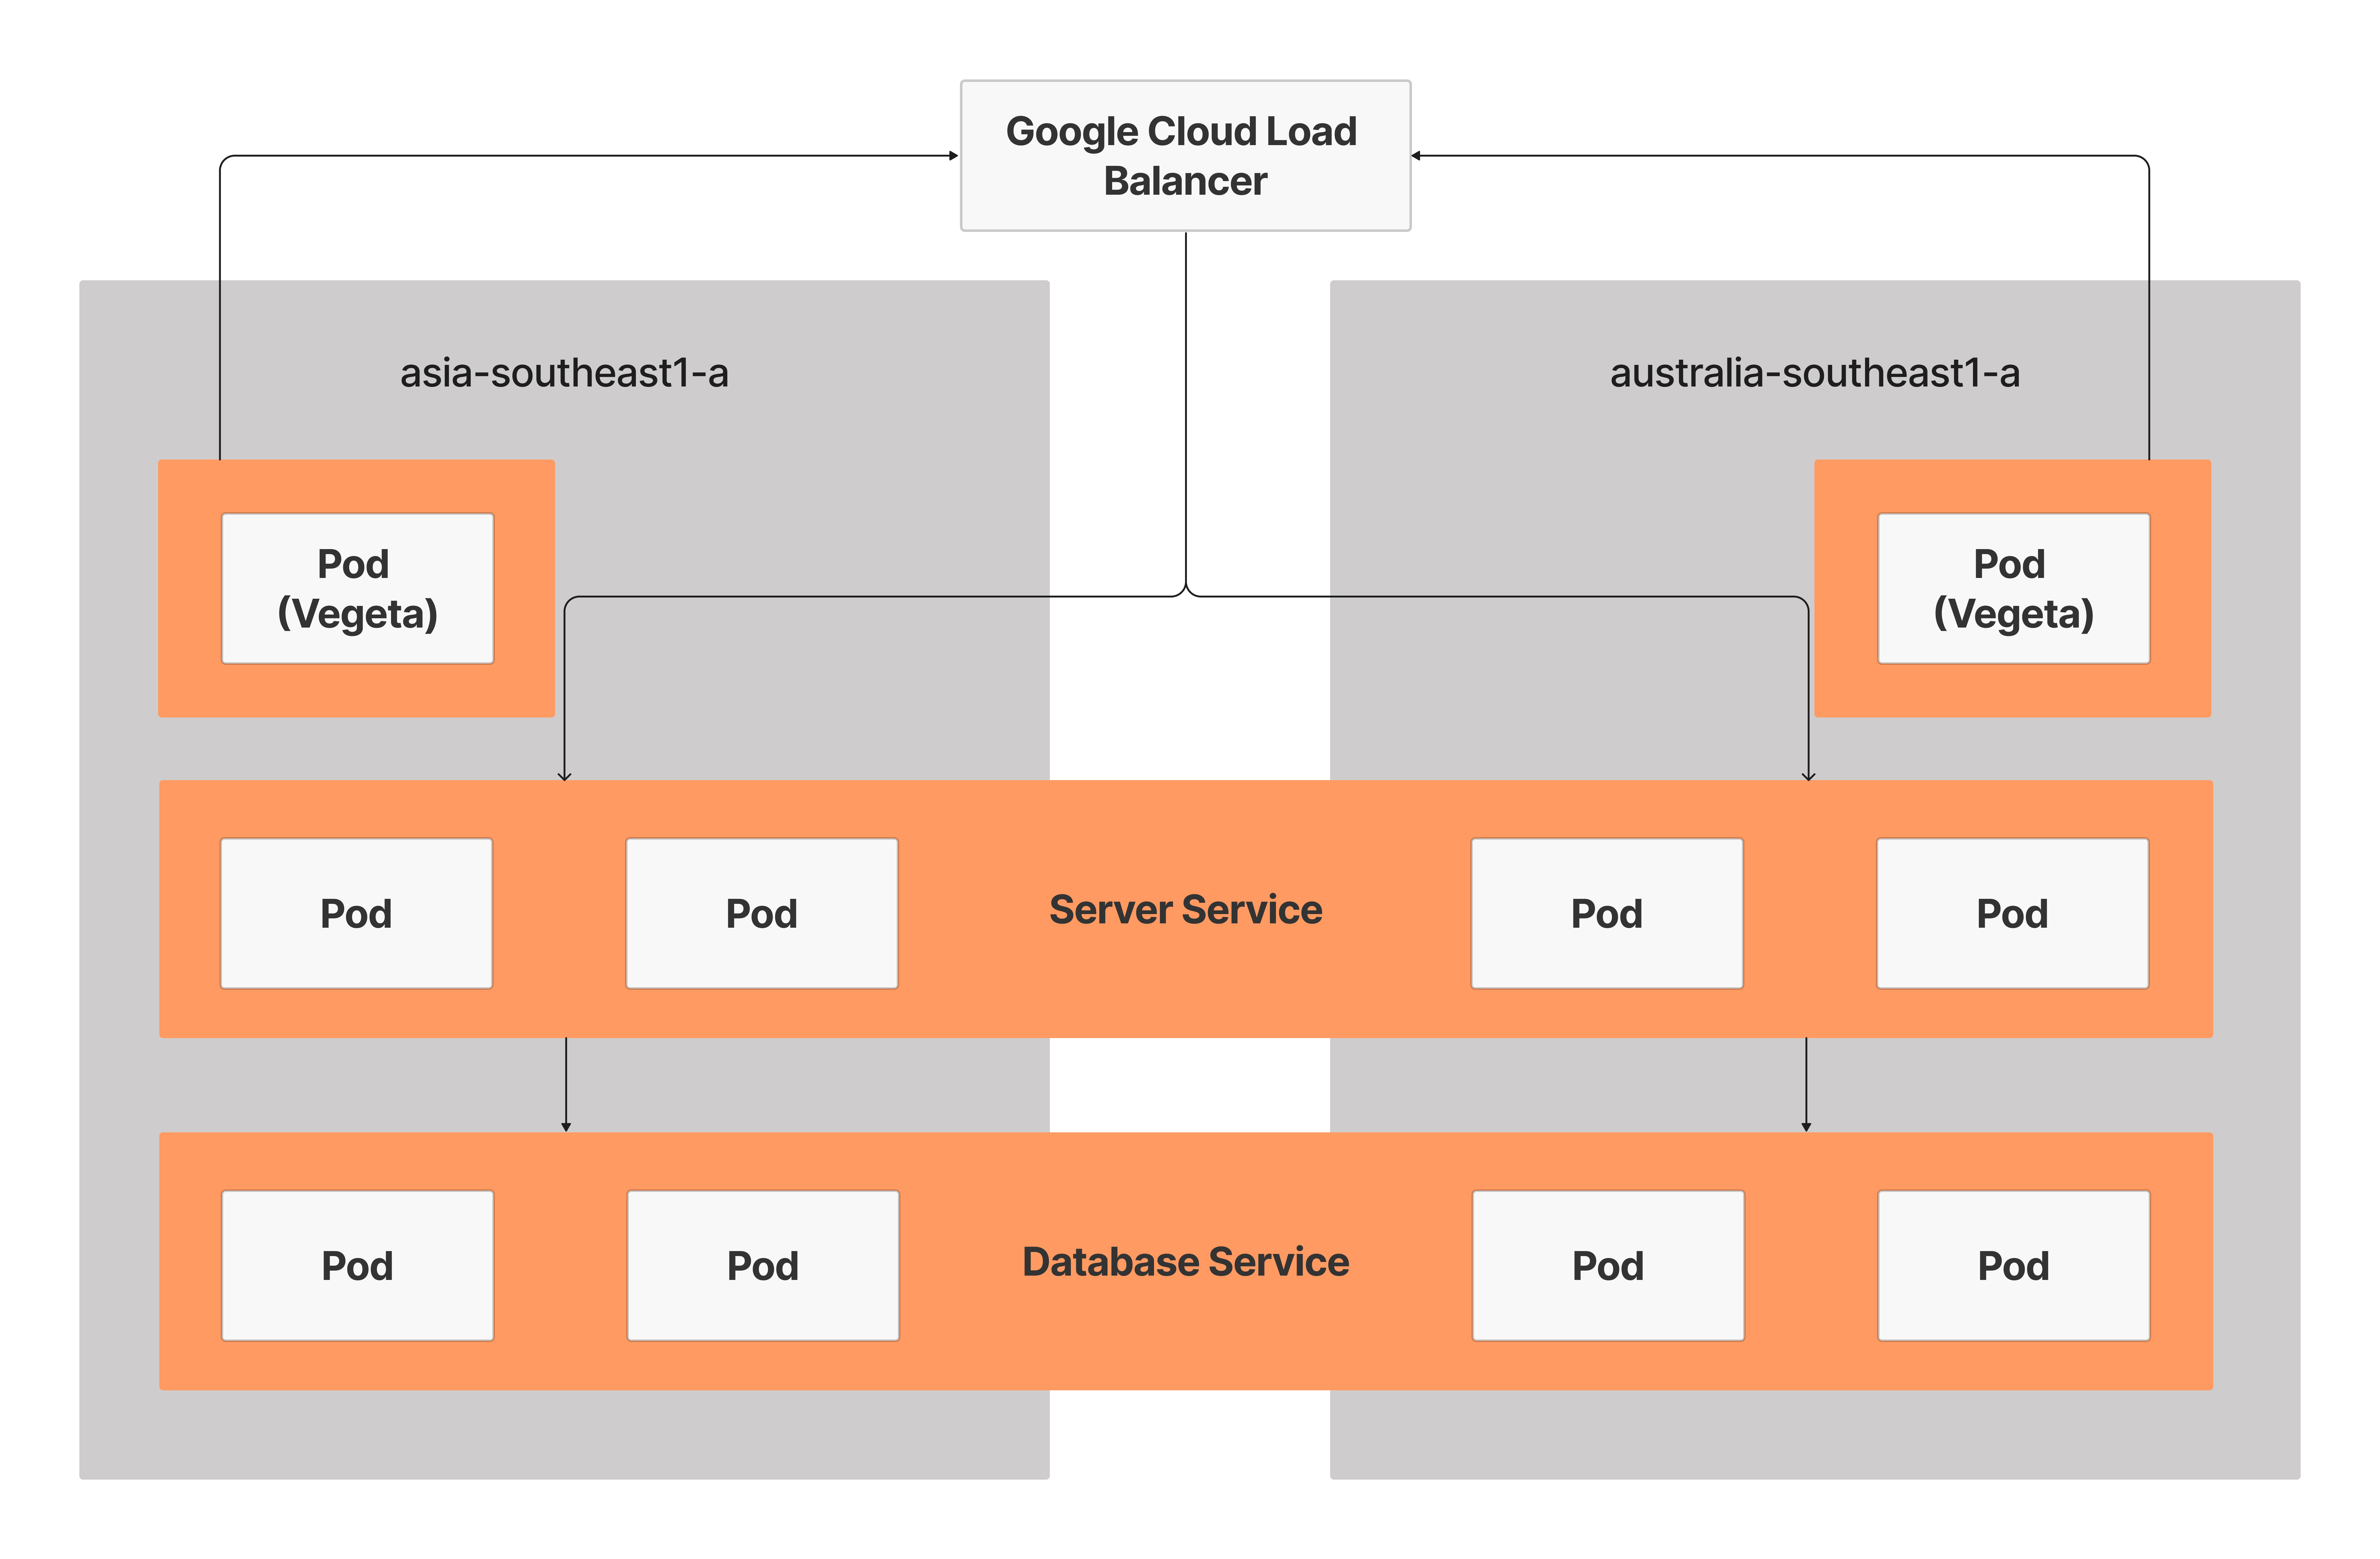
\includegraphics[width=1\textwidth]{assets/diagrams/infra-mcs-mci.png}
	\caption{Geo-distributed Kubernetes clusters infrastructure on the MCS with MCI configuration.}
	\label{fig:infra-mcs-mci}
\end{figure}

% each cluster is installed with Istio control and data plane which
% Next, in the Istio / ASM configuration, installing Istio control and data plane in each cluster enables automatic envoy proxy injection to each pod. We then deploy the DestinationRule resource to configure locality load balancing, which routes traffic to the nearest cluster. Following this, we deployed the Vegeta load testing pod in every region to simulate a request call from a specific region. We decided to use the server layer as a data layer, which is a server connected to each database instance as a solution to the problem of the database layer not being able to be load balanced directly as the database instance is needed on the server runtime. Lastly, the Istio / ASM geo-distributed Kubernetes clusters' infrastructure can be seen in \autoref{fig:infra-istio}.

Next, in the Istio / ASM configuration, we installed the Istio control and data plane in each cluster, which enabled automatic envoy proxy injection to each pod. We then deployed the DestinationRule resource to configure locality load balancing, which routes traffic to the nearest cluster. Following this, we deployed the Vegeta load testing pod in every region to simulate a request call from a specific region. We decided to use the server layer as a data layer, which is a server connected to each database instance because it is not possible to load-balance the database layer directly, as the database instance is a run-time dependency. Lastly, the Istio / ASM geo-distributed Kubernetes clusters' infrastructure can be seen in \autoref{fig:infra-istio}.

% To handle the problem of the database layer not being able to be load balanced directly, as a result of the database instance being needed on the server runtime, a problem that can be handled by having a dedicated data layer which is a server for each database instance

\begin{figure}
	\centering
	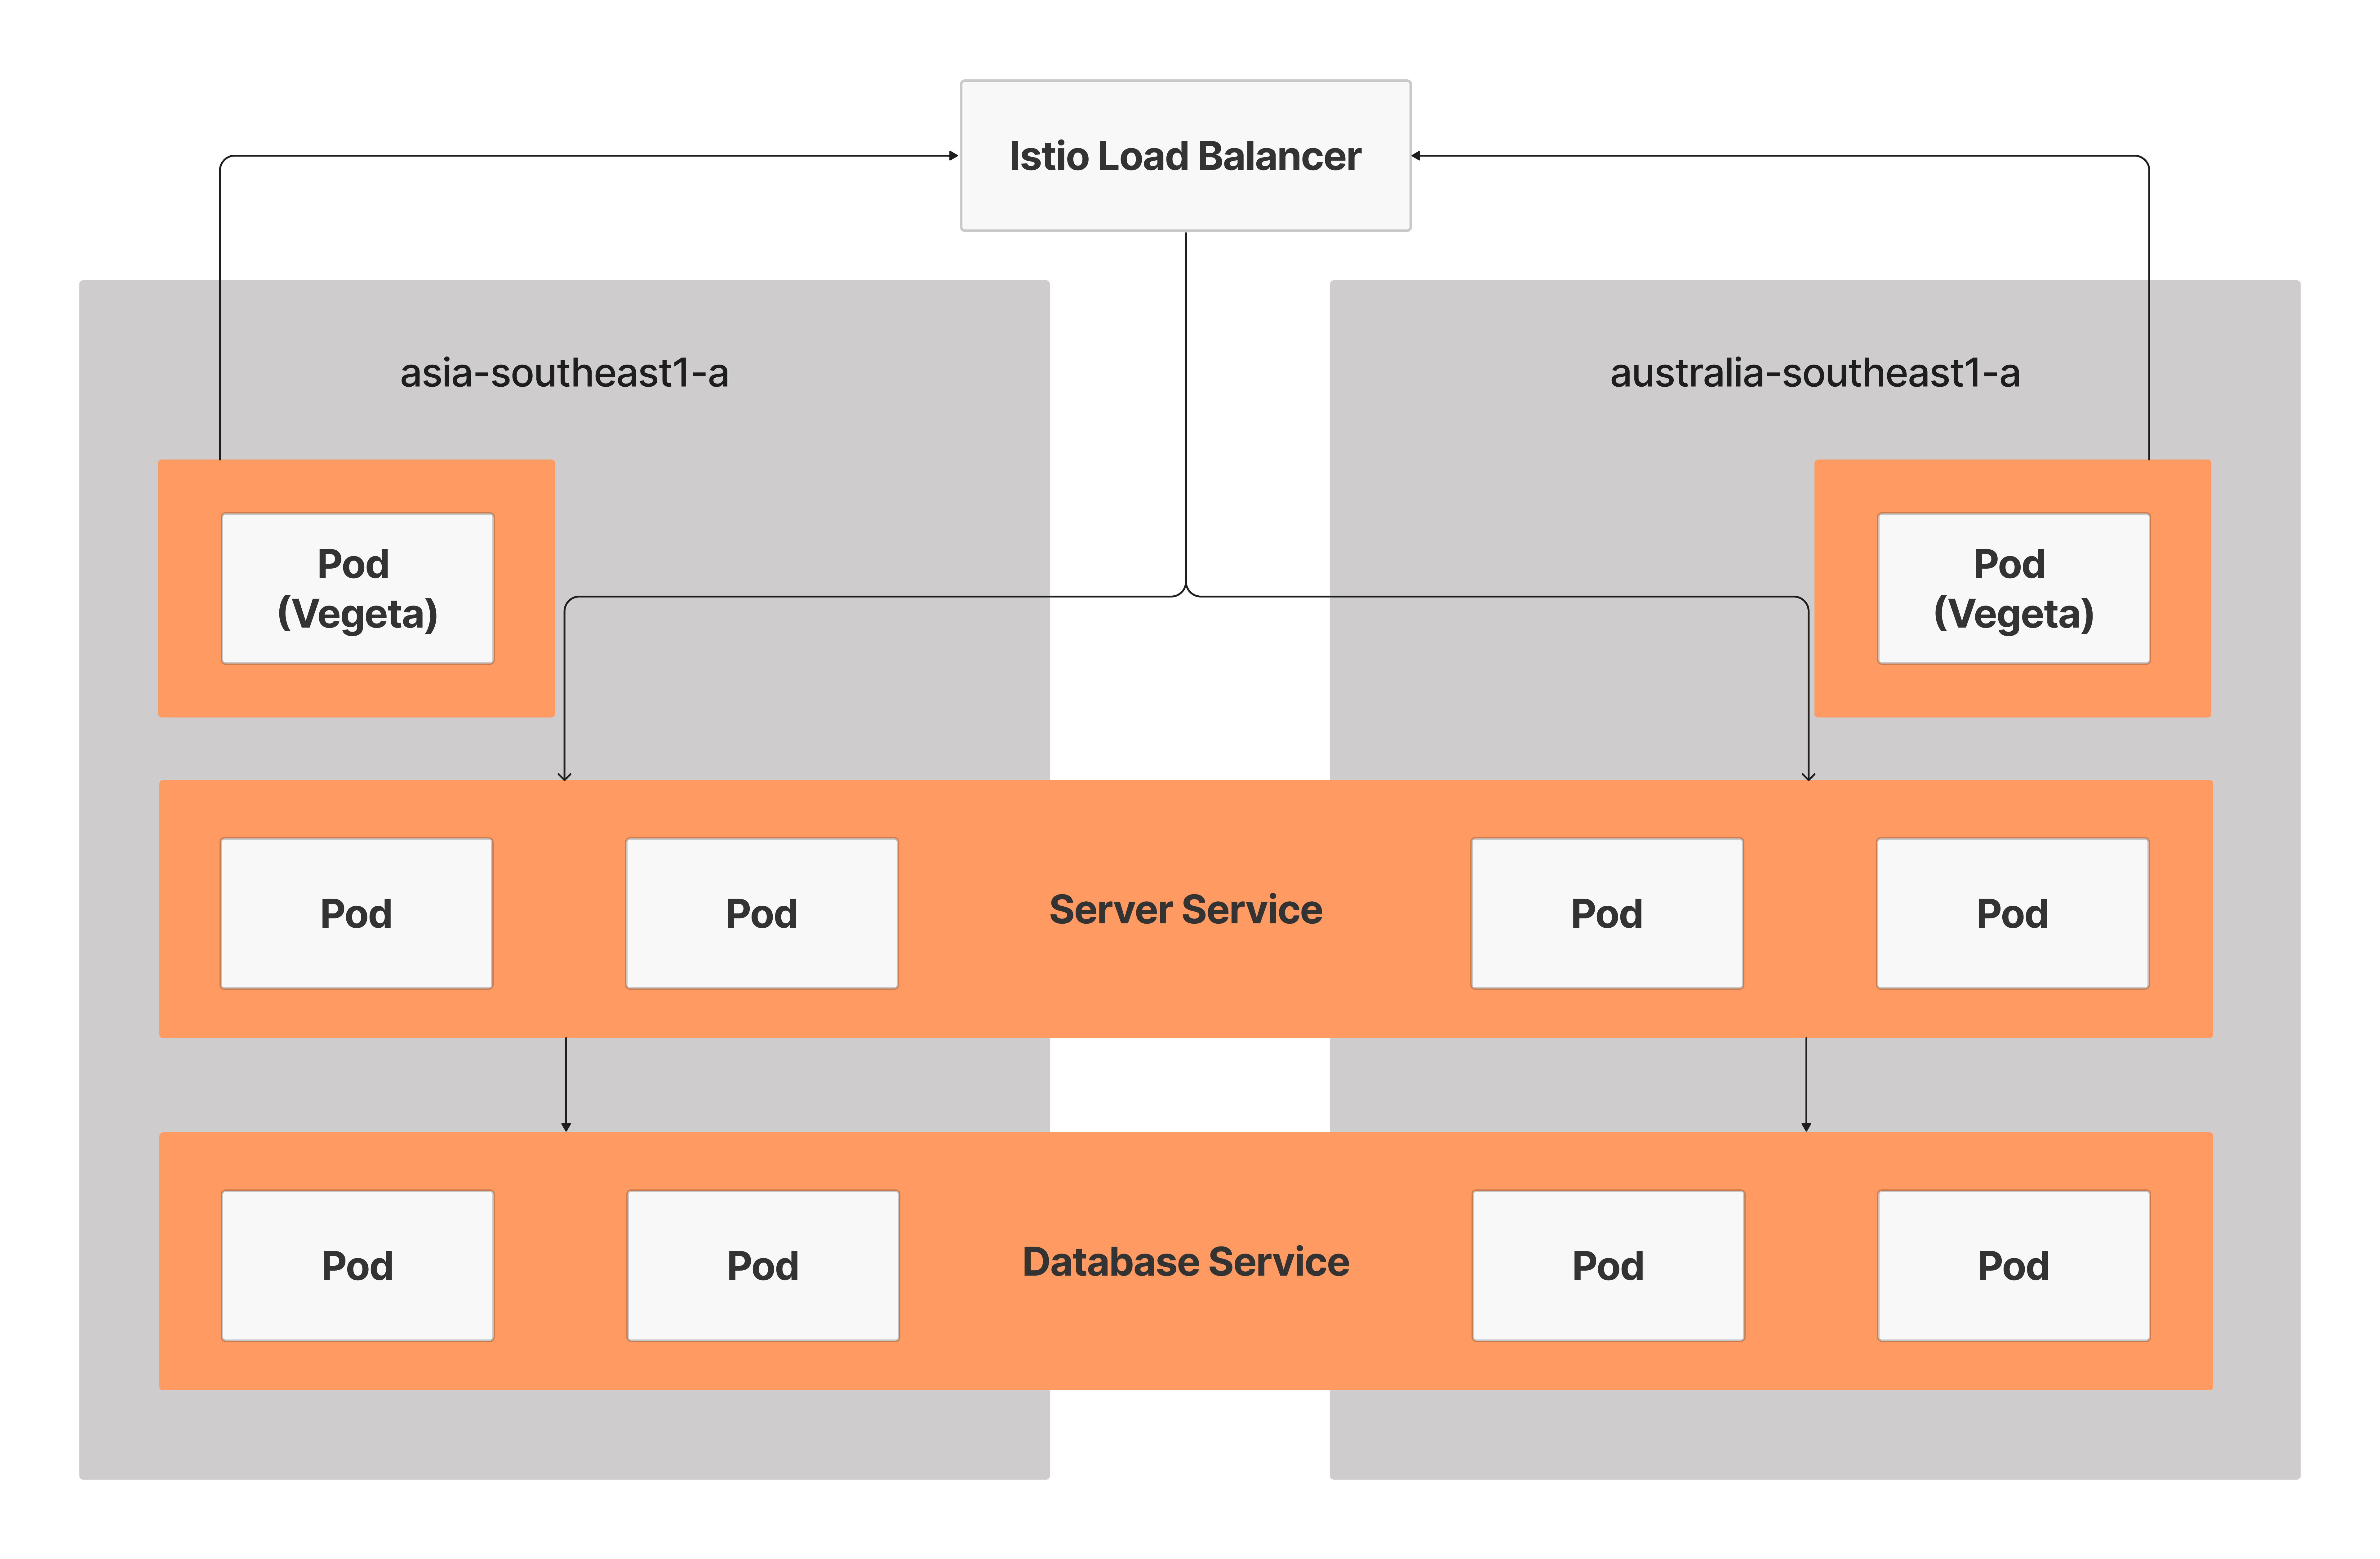
\includegraphics[width=1\textwidth]{assets/diagrams/infra-istio.png}
	\caption{Geo-distributed Kubernetes cluster infrastructure on Istio / ASM configuration.}
	\label{fig:infra-istio}
\end{figure}

\subsection{Kubernetes}
\label{sec:kubernetes-implementation}
% The Kubernetes implementation consists of YAML files which are applied using the \code{kubectl} command-line interface on Google Kubernetes Engine clusters. The Kubernetes implementation for the application can be seen in \autoref{code:client-yaml}, \autoref{code:server-yaml}, and \autoref{code:redis-yaml}
Besides implementing the application, configuring and implementing a Kubernetes architecture was another important step to successfully deploy a geo-distributed cluster web application. Kubernetes implementation and configuration were done through YAML files, which we then applied using the \code{kubectl} command-line interface on Google Kubernetes Engine clusters, where its implementation can be seen in the GitHub repository\footnote{\url{https://github.com/jojonicho/skripsi}}. One of the main selling points of Kubernetes is its networking features, which allow services to communicate with each other and conveniently map each service name defined in the metadata to a URL value that can be provided as an environment variable. For example, to connect the \code{ta-server} service with the \code{ta-redis} service, simply provide \code{ta-redis-service} inside of the server YAML file\footnote{\url{https://github.com/jojonicho/skripsi/blob/master/server.yaml}}, and the redis URL can be accessed inside of the server application as an environment variable.

% is convenient because the service name defined in the metadata section of a service can also be used as a URL mapping to be provided as an environment variable

% \lstinputlisting[language=Yaml, caption=Service and Deployment configuration for ta-client application, label=code:client-yaml]{assets/codes/client.yaml}

% \lstinputlisting[language=Yaml, caption=Service and Deployment configuration for ta-server application, label=code:server-yaml]{assets/codes/server.yaml}

% \lstinputlisting[language=Yaml, caption=Service and Deployment configuration for ta-redis application, label=code:redis-yaml]{assets/codes/redis.yaml}

% \section{Google Kubernetes Engine Cluster Implementation}
% \label{sec:kubernetes-cluster-configuration}
% % \subsection{Kubernetes}

All of the Kubernetes YAML files were applied on Google Kubernetes Engine clusters. Each of the clusters was created using the \code{gcloud} command as shown in \autoref{code:1-create-cluster-se-asia-sh} and each having the configuration shown in \autoref{table:cluster-configuration}.

\vspace{\baselineskip}
% \lstinputlisting[frame=single, language=sh, caption=Google Kubernetes Engine cluster creation script., label=code:1-create-cluster-se-asia-sh, float]{assets/codes/gke/1-create_cluster_se_asia.sh}
\noindent
\begin{minipage}{\linewidth}
\lstinputlisting[frame=single, language=sh, caption=Google Kubernetes Engine cluster creation script., label=code:1-create-cluster-se-asia-sh]{assets/codes/gke/1-create_cluster_se_asia.sh}
\end{minipage}

\begin{table}
	\centering
        \caption{Cluster configurations.}
	\begin{tabular}{|c|c|}
		\hline
		Configuration   & Value (s) \\ \hline
		  % Version & 1.24.9-gke.3200 \\ \hline
            Version & 1.25.7-gke.1000 \\ \hline
            Nodes & 4 \\ \hline
            % Pod Replicas & 1 \\ \hline
            Machine type & e2-standard-4 \\ \hline
	\end{tabular}
	\label{table:cluster-configuration}
\end{table}

% To implement a geo-distributed cluster configuration, regardless of whether it is an MCI with MCI or Isito / ASM implementation, each cluster must be registered to the same fleet. In addition, workload identity needs to be enabled to access Google Cloud services, which can be done by providing a workload pool, as shown in \autoref{code:1.5-fleet-sh}.
In order to implement a geo-distributed cluster configuration, regardless of whether it's an MCI with MCI or Istio / ASM implementation, we first registered each cluster to the same Fleet. In addition, workload identity was enabled to access Google Cloud services, which can be done by providing a workload pool, as shown in \autoref{code:1.5-fleet-sh}.

\vspace{\baselineskip}
\noindent
\begin{minipage}{\linewidth}
% \lstinputlisting[frame=single, language=sh, caption=Fleet registration script., label=code:1.5-fleet-sh, float]{assets/codes/gke/1.5-fleet.sh}
\lstinputlisting[frame=single, language=sh, caption=Fleet registration script., label=code:1.5-fleet-sh]{assets/codes/gke/1.5-fleet.sh}
\end{minipage}

\section{MCS with MCI}
In an MCS with MCI scenario, a config cluster was chosen amongst the available clusters, as shown in \autoref{code:3-config-cluster-sh}, where \code{CLUSTER\_NAME} is the cluster name of the chosen config cluster. The \autoref{code:3-config-cluster-sh} script enabled the deployment of custom resources for MultiClusterService and MultiClusterIngress. The final step was to apply the MCS and MCI resources as shown in \code{MCS.yaml}\footnote{\url{https://github.com/jojonicho/skripsi/blob/master/mcs.yaml}} and \code{MCI.yaml}\footnote{\url{https://github.com/jojonicho/skripsi/blob/master/mci.yaml}} using \code{kubectl} inside of the config cluster.

\vspace{\baselineskip}
\noindent
\begin{minipage}{\linewidth}
% \lstinputlisting[frame=single, language=sh, caption=Config cluster multi-cluster script., label=code:3-config-cluster-sh, float]{assets/codes/gke/3-config-cluster.sh}
\lstinputlisting[frame=single, language=sh, caption=Config cluster multi-cluster script., label=code:3-config-cluster-sh]{assets/codes/gke/3-config-cluster.sh}
\end{minipage}
% \lstinputlisting[language=Python, caption=MCS, label=code:mcs-yaml]{assets/codes/mcs.yaml}
% \lstinputlisting[language=TeX, caption=MCI, label=code:mci-yaml]{assets/codes/mci.yaml}

Deploying a MultiClusterService resource on the config cluster created a derived service resource in each of the clusters registered to a Fleet while deploying the MultiClusterIngress resource created a Virtual IP Address which can be attained using the \code{kubectl describe mci ta-server-ingress} command. To access the URL, we turned off any form of VPN as Google Cloud has connection problems when using them.


\section{Istio / ASM}
% To enable locality load balancing, a DestinationRule resource must be applied, as shown in \autoref{code:destrule-yaml}.
In the Istio / ASM scenario, Anthos Service Mesh was installed in each cluster using \code{asmcli}. Once installed in each cluster, we restarted each deployment pod to enable automatic proxy injection by running the \code{kubectl rollout restart deployment} command. Finally, we applied the DestinationRule resource, as shown in \autoref{code:destrule-yaml}, to enable locality load balancing.

\vspace{\baselineskip}
\noindent
\begin{minipage}{\linewidth}
\lstinputlisting[frame=single, language=YAML, caption=DestinationRule configuration for locality load balancing., label=code:destrule-yaml]{assets/codes/destrule.yaml}
% \lstinputlisting[frame=single, language=YAML, caption=DestinationRule configuration for locality load balancing., label=code:destrule-yaml, float]{assets/codes/destrule.yaml}
\end{minipage}

In addition, we used the DestinationRule resource to configure locality failover, which allowed traffic to be routed to other clusters when a cluster isn't healthy. To enable this, outlier detection was configured, which enabled sidecar proxies to determine if a service is unhealthy.

\section{Performance Testing}
\label{sec:load-testing-implementation}
% The test is done on each region to simulate the request originating from that region by deploying a containerized Vegeta application inside of the respective region
Load testing and stress testing were done using Vegeta, an open-sourced load tester, which we chose for its set of features, mainly the ability to create HTTP requests and report metrics that aligns with the evaluation metrics defined in the methodology of this research. To simulate requests from different regions, we deployed the load testing tool as a containerized Docker image and ran it on each region, allowing the request to originate from a chosen region. We then repeat the same test for every request per second (RPS) configuration, which can be seen in \code{vegeta.sh}\footnote{\url{https://github.com/jojonicho/skripsi/blob/master/tests/vegeta.sh}} and \code{asm-vegeta.sh}\footnote{\url{https://github.com/jojonicho/skripsi/blob/master/tests/asm-vegeta.sh}} for the MCS with MCI configuration and Istio / ASM configuration, respectively.

% Finally, the collection and transformation of data into meaningful human-readable metrics using the \code{vegeta report} command. It can also produce a plot-friendly percentile table by supplying \code{-type=hdrplot} to the report command, as seen in \autoref{code:gen-code-sh}, which allows further analysis of latency percentile distribution.
Finally, we used the \code{vegeta report} command to transform the collected data into human-readable metrics. It can also produce a plot-friendly percentile table by supplying \code{-type=hdrplot} to the report command, as seen in \autoref{code:gen-code-sh}, which allows further analysis of latency percentile distribution.

\vspace{\baselineskip}
\noindent
\begin{minipage}{\linewidth}
% \lstinputlisting[frame=single, language=sh, caption=Service and Deployment configuration for ta-redis application., label=code:gen-code-sh, float]{assets/codes/generate_plot.sh}
\lstinputlisting[frame=single, language=sh, caption=Service and Deployment configuration for ta-redis application., label=code:gen-code-sh]{assets/codes/generate_plot.sh}
\end{minipage}

% There are two kinds of tests done. The first kind of test is to gauge the maximum requests per second (RPS) limit and the second kind is to analyze the effect of increasing the RPS on application performance. The script for load testing is located in \code{vegeta.sh}, \code{vegeta-rate.sh}, \code{asm-vegeta.sh}, and \code{asm-vegeta-rate.sh}.

\clearchapter
%-----------------------------------------------------------------------------%
\chapter{\babLima}
\label{bab:5}
%-----------------------------------------------------------------------------%
% This chapter explains and analyzes the results of the testing done according to the application infrastructure, test scenarios, and evaluation metrics that have been defined.
This chapter discusses the test results and analysis. The discussion includes reliability analysis and performance analysis.

% It seems that the MCS with MCI approach has better performance, which is especially shown during low traffic conditions during the 10 requests / second experiment, where the MCS with MCI approach had no server failures which subsequently causes it to be restarted, while the Istio / ASM have restarted multiple times during the test done in the smallest requests per second variable.


%-----------------------------------------------------------------------------%
\section{Reliability}
\label{sec:analisis}
To evaluate the reliability of geo-distributed clusters, we tested the single-cluster variation as well for comparison. In addition, analyzing the single-cluster results also helps us understand the behavior of each geo-distributed cluster method, mainly its recovery and failover mechanism.

After configuring and testing each scenario, the results can be seen in \autoref{tab:reliability-single-cluster-results} and \autoref{tab:reliability-multi-cluster-results} for single cluster and multi-cluster test results, respectively. The main result that determines reliability is the success ratio for each method.

\begin{table}[h]
\centering
\caption{Single Cluster Reliability Test Results}

\begin{tabular}{|c|c|c|c|}
\hline

\textbf{Method} & \textbf{Location} & \textbf{RPS} & \textbf{Success Ratio} \\ \hline
%  &  &  & \textbf{Min} & \textbf{Mean} & \textbf{Max} &  \\ \hline
%  & & 10 & 2.771 & 3.72 & 6.867 & 100.00\% \\ \cline{3-7}
%  & southeast-asia & 50 & 2.71 & 3.761 & 18.27 & 100.00\% \\ \cline{3-7}
% MCS with & & 100 & 2.546 & 3.851 & 20.348 & 100.00\% \\ \cline{2-7}
% MCI & & 10 & 3.571 & 4.879 & 10.445 & 100.00\% \\ \cline{3-7}
%  & australia & 50 & 3.33 & 4.55 & 14.095 & 100.00\% \\ \cline{3-7}
%  & & 100 & 3.29 & 4.623 & 17.547 & 100.00\% \\ \hline
%  & & 10 & 1.745 & 3.709 & 52.527 & 62.67\% \\ \cline{3-7}
%  & southeast-asia & 50 & 1.512 & 3.232 & 35.926 & 71.87\% \\ \cline{3-7}
% Istio / & & 100 & 1.426 & 2.912 & 44.033 & 71.93\% \\ \cline{2-7}
% ASM & & 10 & 1.783 & 32.38 & 127.82 & 33.33\% \\ \cline{3-7}
%  & australia & 50 & 1.696 & 10.959 & 114.222 & 34.67\% \\ \cline{3-7}
%  & & 100 & 1.453 & 7.383 & 289.035 & 30.07\% \\ \hline

 & & 10 & 100.00\% \\ \cline{3-4}
 & southeast-asia & 50 & 100.00\% \\ \cline{3-4}
MCS with & & 100 & 100.00\% \\ \cline{2-4}
MCI & & 10 & 100.00\% \\ \cline{3-4}
 & australia & 50 & 100.00\% \\ \cline{3-4}
 & & 100 & 100.00\% \\ \hline
 & & 10 & 62.67\% \\ \cline{3-4}
 & southeast-asia & 50 & 71.87\% \\ \cline{3-4}
Istio / & & 100 & 71.93\% \\ \cline{2-4}
ASM & & 10 & 33.33\% \\ \cline{3-4}
 & australia & 50 & 34.67\% \\ \cline{3-4}
 & & 100 & 30.07\% \\ \hline

\end{tabular}
\label{tab:reliability-single-cluster-results}
\end{table}

From the single cluster test results, it can be seen that MCS with MCI performs better than Istio / ASM as it is able to handle up to 100 requests per second. This can be explained by the added complexity that Istio brings inside of a Kubernetes architecture, mainly having to inject the Envoy sidecar in each pod. This results in more resources and time required, especially in the case of server recovery during high traffic. In addition, the error response set, as seen in \autoref{pic:error-code-0}, confirms this, as all of the errors have a response code of 0, which means that the requests weren't sent at all, as the server was busy restarting. Server restarts are an expected behavior, as it happens when a server is overloaded, as indicated by an error response code, and are necessary to return a server to a healthy state. Furthermore, the internal state of the pod can be seen in \autoref{pic:readiness-probe-fail}, where a readiness probe, which is done to check if a pod is healthy, failed as it has not recovered. This results in the connection refused error received by the client.

\begin{figure}
	\centering
	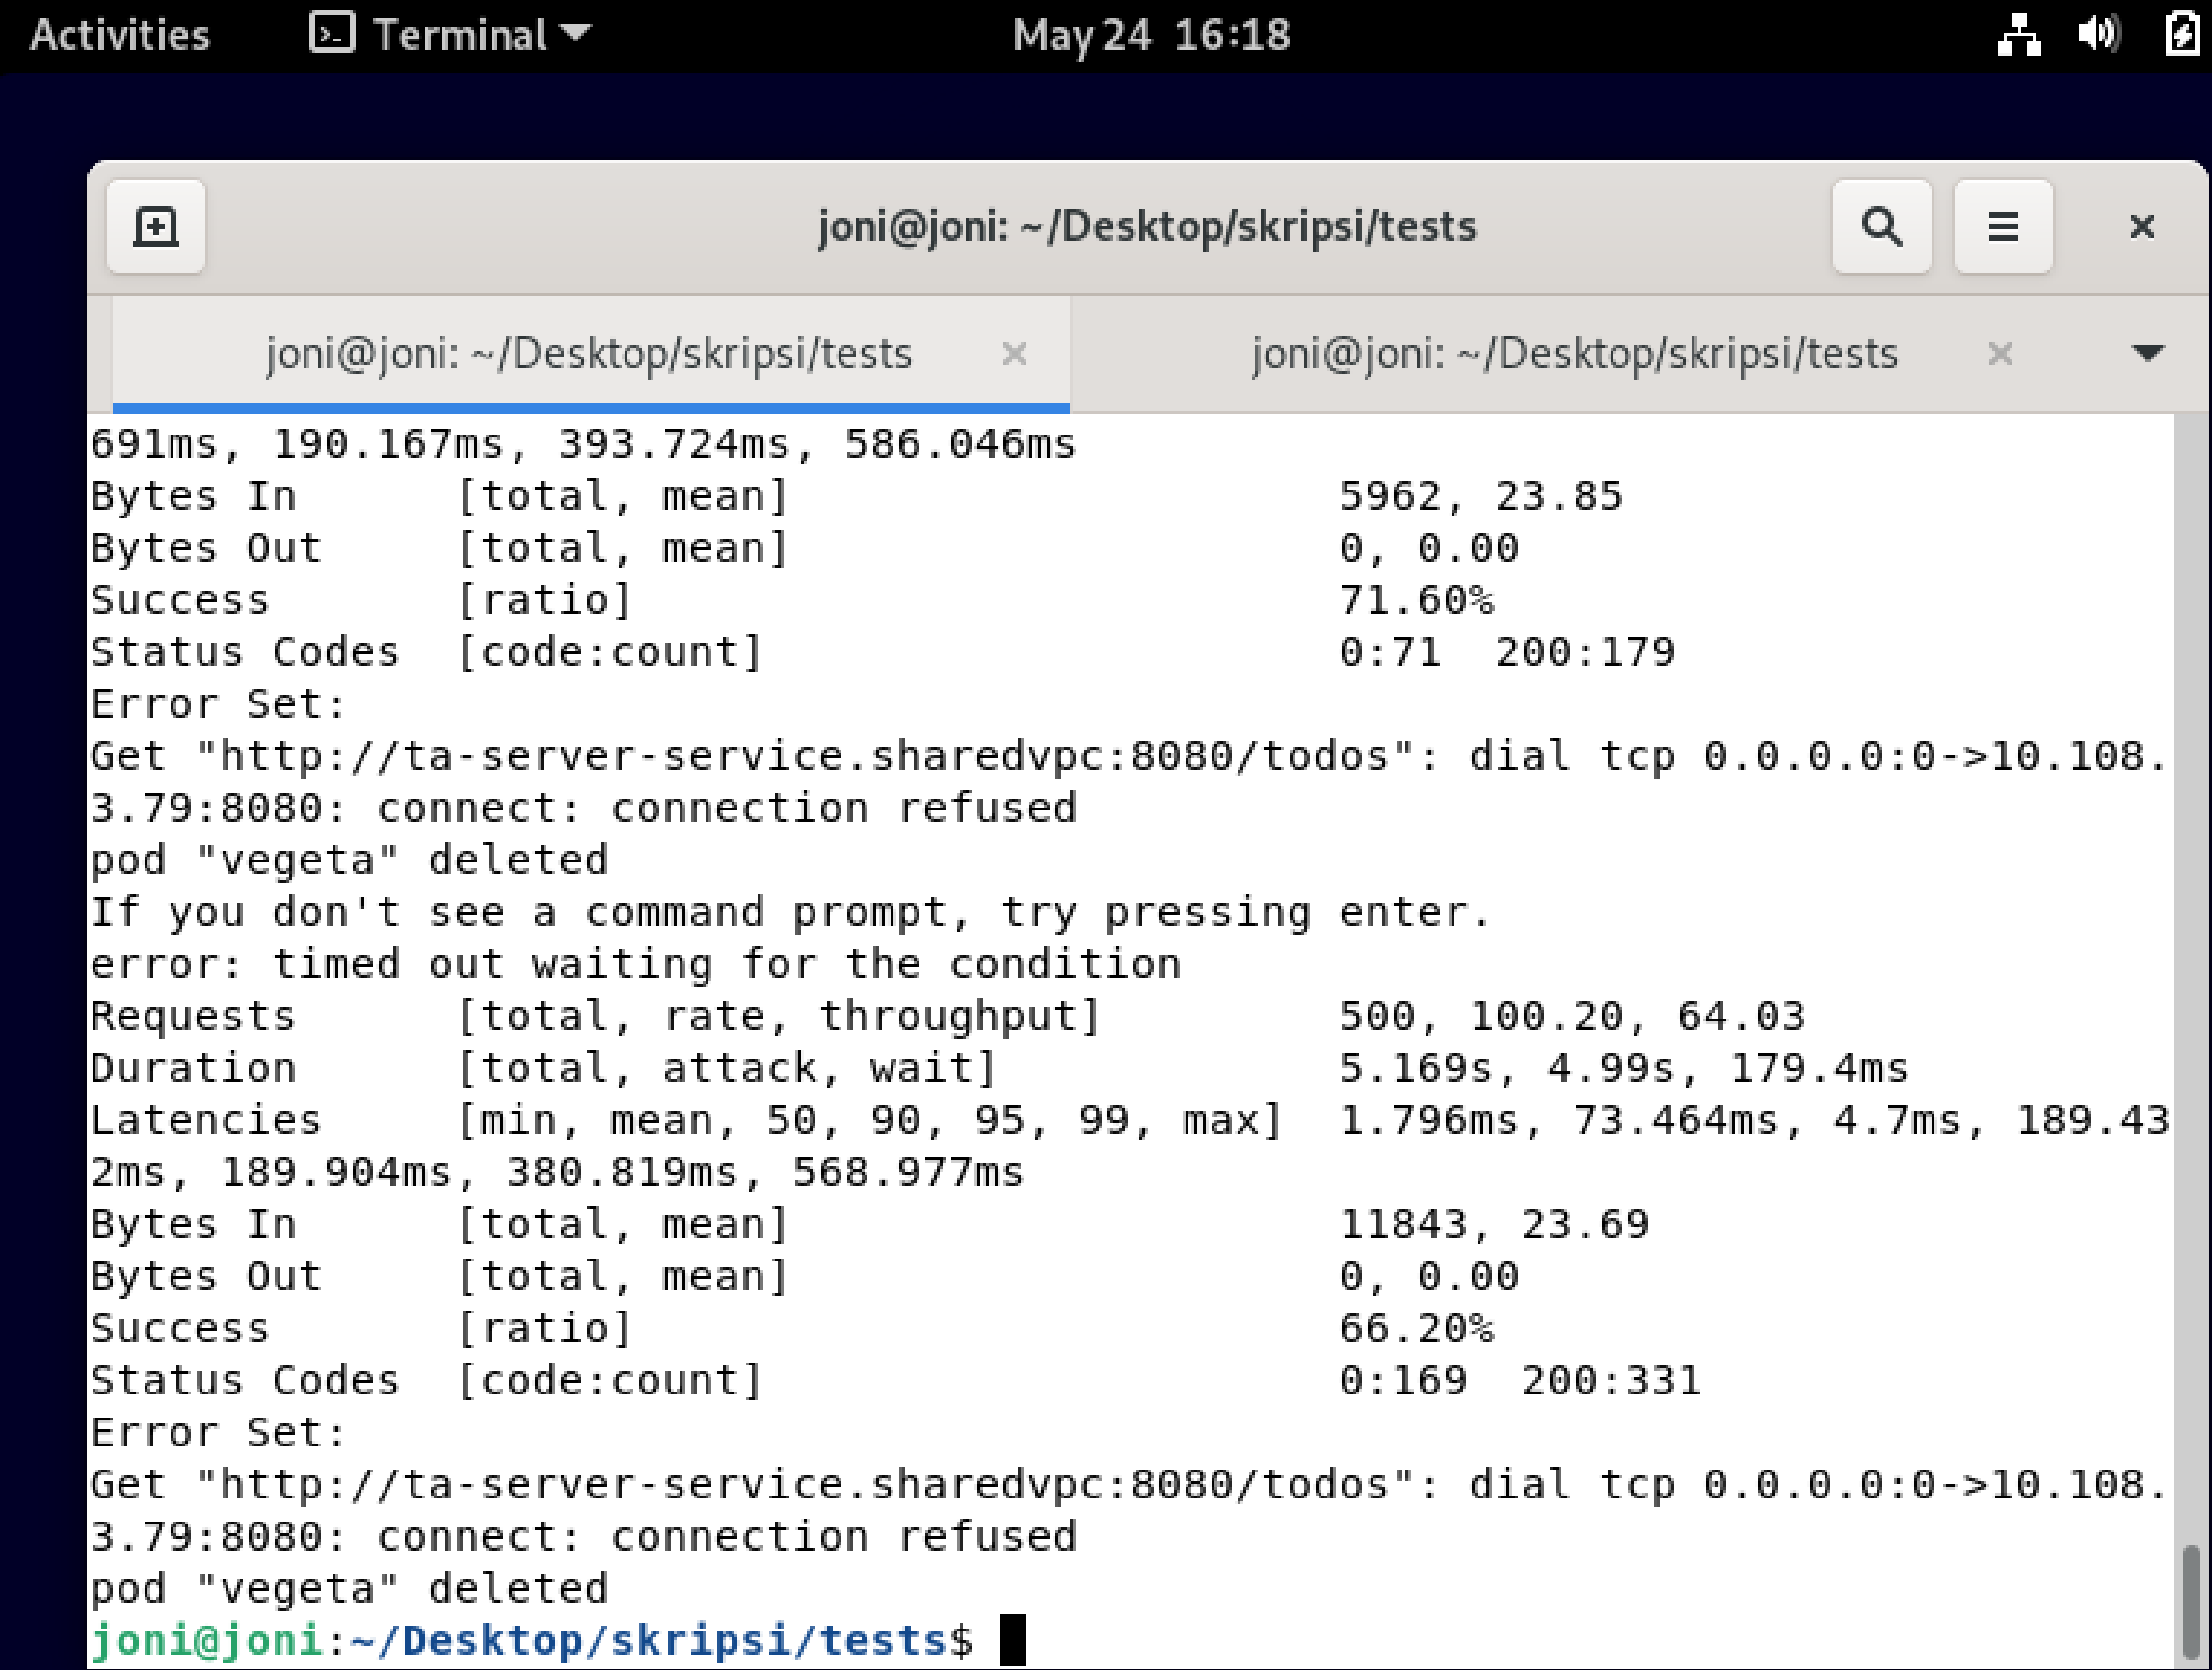
\includegraphics[width=1\textwidth]{assets/pics/error-code-0.png}
	\caption{Testing report with HTTP code 0 connection refused response.}
	\label{pic:error-code-0}
\end{figure}
\begin{figure}
	\centering
	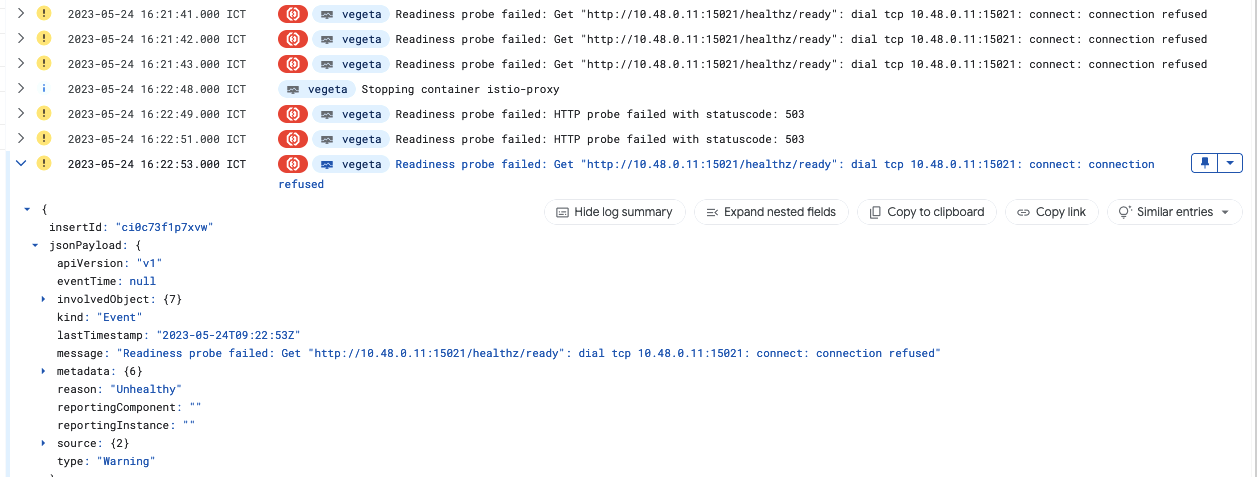
\includegraphics[width=1\textwidth]{assets/pics/readiness-probe-fail.png}
	\caption{Pod logs showing readiness probe fail.}
	\label{pic:readiness-probe-fail}
\end{figure}

There is also a discrepancy between the cluster's success ratio on Istio / ASM, where southeast-asia's has at least 2 times higher success ratio than its australia counterpart. As there are virtually no differences between the cluster's methods, this is perhaps an issue on the Google Cloud Platform's part, whether intended or not.


\begin{table}[h]
\centering
\caption{Multi-Cluster Reliability Test Results}

\begin{tabular}{|c|c|c|c|}
\hline

% \textbf{Method} & \textbf{Location} & \textbf{RPS} & \multicolumn{3}{c|}{\textbf{Latency (ms)}} & \textbf{Success Ratio} \\ \cline{4-6}
%  &  &  & \textbf{Min} & \textbf{Mean} & \textbf{Max} &  \\ \hline

\textbf{Method} & \textbf{Location} & \textbf{RPS} & \textbf{Success Ratio} \\ \hline
% TC 1 RES

%  & & 10 & 2.841179 & 3.687702 & 7.261602 & 100.00\% \\ \cline{3-7}
%  & southeast-asia & 50 & 2.48722 & 3.142731 & 6.367496 & 100.00\% \\ \cline{3-7}
% MCS with & & 100 & 3.835657 & 4.369947 & 8.858507 & 100.00\% \\ \cline{2-7}
% MCI & & 10 & 3.560003 & 4.743905 & 8.014017 & 100.00\% \\ \cline{3-7}
%  & australia & 50 & 3.938387 & 5.050108 & 10.318062 & 100.00\% \\ \cline{3-7}
%  & & 100 & 3.426384 & 4.202816 & 13.548108 & 100.00\% \\ \hline
%  & & 10 & 1.782431 & 3.627414 & 52.527168 & 40.00\% \\ \cline{3-7}
%  & southeast-asia & 50 & 1.511889 & 3.252973 & 33.364391 & 73.20\% \\ \cline{3-7}
% Istio / & & 100 & 1.48613 & 2.866272 & 33.372959 & 71.60\% \\ \cline{2-7}
% ASM & & 10 & 1.804273 & 29.992081 & 127.820017 & 32.00\% \\ \cline{3-7}
%  & australia & 50 & 1.721937 & 9.974838 & 96.424287 & 41.20\% \\ \cline{3-7}
%  & & 100 & 1.688115 & 5.778561 & 104.033348 & 31.40\% \\ \hline

% ALL TC RES
%  & & 10 & 2.841 & 3.836 & 8.219 & 100.00\% \\ \cline{3-7}
%  & southeast-asia & 50 & 2.487 & 3.657 & 8.992 & 100.00\% \\ \cline{3-7}
% MCS with & & 100 & 2.434 & 3.96 & 14.286 & 100.00\% \\ \cline{2-7}
% MCI & & 10 & 3.56 & 4.723 & 8.819 & 100.00\% \\ \cline{3-7}
%  & australia & 50 & 3.261 & 4.366 & 10.318 & 100.00\% \\ \cline{3-7}
%  & & 100 & 3.178 & 4.097 & 14.572 & 100.00\% \\ \hline
%  & & 10 & 1.745 & 3.709 & 52.527 & 62.67\% \\ \cline{3-7}
%  & southeast-asia & 50 & 1.512 & 3.232 & 35.926 & 71.87\% \\ \cline{3-7}
% Istio / & & 100 & 1.426 & 2.912 & 44.033 & 71.93\% \\ \cline{2-7}
% ASM & & 10 & 1.783 & 32.38 & 127.82 & 33.33\% \\ \cline{3-7}
%  & australia & 50 & 1.696 & 10.959 & 114.222 & 34.67\% \\ \cline{3-7}
%  & & 100 & 1.453 & 7.383 & 289.035 & 30.07\% \\ \hline

% FIXED LB
%  & & 10 & 2.841 & 3.836 & 8.219 & 100.00\% \\ \cline{3-7}
%  & southeast-asia & 50 & 2.487 & 3.657 & 8.992 & 100.00\% \\ \cline{3-7}
% MCS with & & 100 & 2.434 & 3.96 & 14.286 & 100.00\% \\ \cline{2-7}
% MCI & & 10 & 3.56 & 4.723 & 8.819 & 100.00\% \\ \cline{3-7}
%  & australia & 50 & 3.261 & 4.366 & 10.318 & 100.00\% \\ \cline{3-7}
%  & & 100 & 3.178 & 4.097 & 14.572 & 100.00\% \\ \hline
%  & & 10 & 3.497 & 35.543 & 103.985 & 100.00\% \\ \cline{3-7}
%  & southeast-asia & 50 & 3.594 & 10.724 & 103.524 & 100.00\% \\ \cline{3-7}
% Istio / & & 100 & 3.158 & 6.52 & 293.551 & 100.00\% \\ \cline{2-7}
% ASM & & 10 & 3.509 & 4.42 & 58.857 & 100.00\% \\ \cline{3-7}
%  & australia & 50 & 2.967 & 3.868 & 10.506 & 100.00\% \\ \cline{3-7}
%  & & 100 & 2.789 & 7.735 & 291.411 & 100.00\% \\ \hline
 
%  & & 10 & 1.745 & 3.709 & 52.527 & 62.67\% \\ \cline{3-7}
%  & southeast-asia & 50 & 1.512 & 3.232 & 35.926 & 71.87\% \\ \cline{3-7}
% Istio / ASM & & 100 & 1.426 & 2.912 & 44.033 & 71.93\% \\ \cline{2-7}
% (Single Cluster) & & 10 & 1.783 & 32.38 & 127.82 & 33.33\% \\ \cline{3-7}
%  & australia & 50 & 1.696 & 10.959 & 114.222 & 34.67\% \\ \cline{3-7}
%  & & 100 & 1.453 & 7.383 & 289.035 & 30.07\% \\ \hline

 & & 10 & 100.00\% \\ \cline{3-4}
 & southeast-asia & 50 & 100.00\% \\ \cline{3-4}
MCS with & & 100 & 100.00\% \\ \cline{2-4}
MCI & & 10 & 100.00\% \\ \cline{3-4}
 & australia & 50 & 100.00\% \\ \cline{3-4}
 & & 100 & 100.00\% \\ \hline
 & & 10 & 100.00\% \\ \cline{3-4}
 & southeast-asia & 50 & 100.00\% \\ \cline{3-4}
Istio / & & 100 & 100.00\% \\ \cline{2-4}
ASM & & 10 & 100.00\% \\ \cline{3-4}
 & australia & 50 & 100.00\% \\ \cline{3-4}
 & & 100 & 100.00\% \\ \hline

\end{tabular}
\label{tab:reliability-multi-cluster-results}
\end{table}

In contrast to single-cluster performance, multi-cluster performance seems to have fixed the reliability issue of Istio / ASM, where it can withstand 100 requests per second without a single failure. At the same time, the MCS with MCI maintains its perfect response ratio.

In addition, the server inside of a MCS with MCI method is able to handle 10 requests per second without restarting and only needs server recovery for 50 requests per second and above. In contrast, the server inside the Istio / ASM method needed to restart even during the lowest request per second configuration. This implies that a single cluster Istio / ASM may not be the most suitable geo-distributed approach for production-level applications, as it is unable to handle pedestrian-level traffic without inducing downtime on the servers. Therefore, it appears that MCS with MCI is more reliable than Istio / ASM for a single cluster configuration. It is advisable for Istio / ASM adopters to maximize its reliability by deploying services to multiple clusters and enabling the failover feature. Furthermore, there seems to be a problem with the Istio / ASM approach, where the failover feature of locality load balancing won't work with clients without a Service resource. This results in only one cluster responding to all of the requests without utilizing the other clusters.

In conclusion, the geo-distributed Kubernetes architecture is an effective way to increase the reliability of web applications, as it provides a connected network of clusters that serves as a failover when a cluster is experiencing downtime. There are also performance benefits to this, which we will see in \autoref{sec:5-perf}.

% \end{minipage}
% \begin{minipage}{.45\textwidth}
% \centering
% \begin{tabular}{|c|c|}
% \hline
% \textbf{Metric} & \textbf{Value} \\ \hline
% Success Ratio & 71.60\% \\ \hline
% \end{tabular}
% \caption{Success Metrics}
% \label{tab:success}
% \end{minipage}

% \todo{Tulis penjelasan terkait \tab~\ref{table:sample} di sini. Jika Anda hanya menunjukkan data, pembaca tidak akan tahu apakah data tersebut berharga.}


\section{Performance}
\label{sec:5-perf}

Istio / ASM's results may seem to be better for the single cluster configuration, especially if you compare the minimum latencies of each configuration from each method. However, this is simply the result of requests not being sent, resulting in it having a latency of under 2 milliseconds.

By comparing the minimum, average, and maximum latency of both configurations, as shown in \autoref{tab:multi-cluster-performance-results}, it can be seen that MCS with MCI has lower latency overall. Another important observation is the latency deviation produced by the Istio / ASM approach, where it may fluctuate to just under 300 milliseconds. This is a 171\% to 4385\% increase compared to MCS with MCI with a much more stable percentage increase between 136\% to 255\%.

\begin{table}[h]
\begin{adjustwidth}{-2cm}{-2cm}
 % \centering\makebox[\textwidth]
%  \centering\makebox{\textwidth}{}
%  % \centerline
%  {\resizebox{1.5\textwidth}{!}{%
\centering
\caption{Multi-Cluster Performance Test Results}

\begin{tabular}{|c|c|c|c|c|c|c|c|c|c|c|c|}
\hline

% \textbf{Method} & \textbf{Location} & \textbf{RPS} & \multicolumn{3}{c|}{\textbf{Latency (ms)}} & \textbf{Success Ratio} \\ \cline{4-6}
 % &  &  & \textbf{Min} & \textbf{Mean} & \textbf{Max} &  \\ \hline

% & & & & & \multicolumn{2}{c|}{\textbf{MCS with MCI}} & \multicolumn{2}{c|}{\textbf{Istio / ASM}}\\ \cline{5-6}
% \textbf{Method} & \textbf{Location} & \textbf{Test} & \textbf{RPS} & \multicolumn{2}{c|}{\textbf{Latency (ms)}} & \\ \cline{5-6}
%  &  & \textbf{Case} &  & \textbf{50th} & \textbf{95th} \\ \hline

% & & & \multicolumn{4}{c|}{\textbf{Latency (ms)}} \\ \cline{4-7}
% \textbf{Location} & \textbf{Test} & \textbf{RPS} & \multicolumn{2}{c|}{\textbf{50th}} & \multicolumn{2}{c|}{\textbf{95th}} \\ \cline{4-7}
% &  &  & \textbf{MCS} & \textbf{ASM} & \textbf{MCS} & \textbf{ASM} \\ \hline

% & & \multicolumn{10}{c|}{\textbf{Latency (ms)}} \\ \cline{3-12}
% \textbf{Location} & \textbf{RPS} & \multicolumn{2}{c|}{\textbf{50th}} & \multicolumn{2}{c|}{\textbf{95th}} & \multicolumn{2}{c|}{\textbf{Min}} & \multicolumn{2}{c|}{\textbf{Mean}}  & \multicolumn{2}{c|}{\textbf{Max}} \\ \cline{3-12}
% &  &  \textbf{MCS} & \textbf{ASM} & \textbf{MCS} & \textbf{ASM} & \textbf{MCS} & \textbf{ASM} & \textbf{MCS} & \textbf{ASM} & \textbf{MCS} & \textbf{ASM} \\ \hline

& & \multicolumn{10}{c|}{\textbf{Latency (ms)}} \\ \cline{3-12}
\textbf{Location} & \textbf{RPS} & \multicolumn{2}{c|}{\textbf{Min}} & \multicolumn{2}{c|}{\textbf{Median}} & \multicolumn{2}{c|}{\textbf{Mean}} & \multicolumn{2}{c|}{\textbf{95th}}  & \multicolumn{2}{c|}{\textbf{Max}} \\ \cline{3-12}
&  &  \textbf{MCS} & \textbf{ASM} & \textbf{MCS} & \textbf{ASM} & \textbf{MCS} & \textbf{ASM} & \textbf{MCS} & \textbf{ASM} & \textbf{MCS} & \textbf{ASM} \\ \hline

%  & southeast-asia & 1 & 10 & 3.37 & 5.593 \\ \cline{3-6}
%  & southeast-asia & 1 & 50 & 3.017 & 4.111 \\ \cline{3-6}
%  & southeast-asia & 1 & 100 & 4.286 & 4.861 \\ \cline{3-6}
%  & southeast-asia & 2 & 10 & 3.593 & 7.588 \\ \cline{3-6}
%  & southeast-asia & 2 & 50 & 3.322 & 4.033 \\ \cline{3-6}
%  & southeast-asia & 2 & 100 & 4.033 & 4.808 \\ \cline{3-6}
%  & southeast-asia & 3 & 10 & 3.47 & 5.068 \\ \cline{3-6}
%  & southeast-asia & 3 & 50 & 4.052 & 6.846 \\ \cline{3-6}
% MCS with & southeast-asia & 3 & 100 & 3.471 & 4.084 \\ \cline{2-6}
% MCI & australia & 1 & 10 & 4.492 & 6.693 \\ \cline{3-6}
%  & australia & 1 & 50 & 4.8 & 7.248 \\ \cline{3-6}
%  & australia & 1 & 100 & 3.958 & 5.943 \\ \cline{3-6}
%  & australia & 2 & 10 & 4.042 & 5.603 \\ \cline{3-6}
%  & australia & 2 & 50 & 3.799 & 5.355 \\ \cline{3-6}
%  & australia & 2 & 100 & 3.919 & 5.767 \\ \cline{3-6}
%  & australia & 3 & 10 & 4.745 & 6.946 \\ \cline{3-6}
%  & australia & 3 & 50 & 3.794 & 5.399 \\ \cline{3-6}
%  & australia & 3 & 100 & 3.797 & 5.156 \\ \hline
%  & southeast-asia & 1 & 10 & 4.2 & 4.826 \\ \cline{3-6}
%  & southeast-asia & 1 & 50 & 4.529 & 5.047 \\ \cline{3-6}
%  & southeast-asia & 1 & 100 & 4.26 & 96.766 \\ \cline{3-6}
%  & southeast-asia & 2 & 10 & 97.476 & 98.198 \\ \cline{3-6}
%  & southeast-asia & 2 & 50 & 4.464 & 97.65 \\ \cline{3-6}
%  & southeast-asia & 2 & 100 & 4.134 & 4.606 \\ \cline{3-6}
%  & southeast-asia & 3 & 10 & 4.42 & 4.908 \\ \cline{3-6}
%  & southeast-asia & 3 & 50 & 4.499 & 5.402 \\ \cline{3-6}
% Istio / & southeast-asia & 3 & 100 & 3.969 & 4.532 \\ \cline{2-6}
% ASM & australia & 1 & 10 & 3.951 & 4.686 \\ \cline{3-6}
%  & australia & 1 & 50 & 3.649 & 4.089 \\ \cline{3-6}
%  & australia & 1 & 100 & 3.582 & 4.074 \\ \cline{3-6}
%  & australia & 2 & 10 & 3.9 & 4.371 \\ \cline{3-6}
%  & australia & 2 & 50 & 3.977 & 4.471 \\ \cline{3-6}
%  & australia & 2 & 100 & 3.676 & 4.236 \\ \cline{3-6}
%  & australia & 3 & 10 & 3.902 & 4.554 \\ \cline{3-6}
%  & australia & 3 & 50 & 3.831 & 4.253 \\ \cline{3-6}
%  & australia & 3 & 100 & 3.621 & 96.294 \\ \hline

% southeast-asia & 1 & 10 & \textbf{3.37} & 4.2 & 5.593 & \textbf{4.826} \\ \cline{4-7}
% southeast-asia & 1 & 50 & \textbf{3.017} & 4.529 & \textbf{4.111} & 5.047 \\ \cline{4-7}
% southeast-asia & 1 & 100 & 4.286 & \textbf{4.26} & \textbf{4.861} & 96.766 \\ \cline{4-7}
% southeast-asia & 2 & 10 & \textbf{3.593} & 97.476 & \textbf{7.588} & 98.198 \\ \cline{4-7}
% southeast-asia & 2 & 50 & \textbf{3.322} & 4.464 & \textbf{4.033} & 97.65 \\ \cline{4-7}
% southeast-asia & 2 & 100 & \textbf{4.033} & 4.134 & 4.808 & \textbf{4.606} \\ \cline{4-7}
% southeast-asia & 3 & 10 & \textbf{3.47} & 4.42 & 5.068 & \textbf{4.908} \\ \cline{4-7}
% southeast-asia & 3 & 50 & \textbf{4.052} & 4.499 & 6.846 & \textbf{5.402} \\ \cline{4-7}
% southeast-asia & 3 & 100 & \textbf{3.471} & 3.969 & \textbf{4.084} & 4.532 \\ \cline{4-7}
% australia & 1 & 10 & 4.492 & \textbf{3.951} & 6.693 & \textbf{4.686} \\ \cline{4-7}
% australia & 1 & 50 & 4.8 & \textbf{3.649} & 7.248 & \textbf{4.089} \\ \cline{4-7}
% australia & 1 & 100 & 3.958 & \textbf{3.582} & 5.943 & \textbf{4.074} \\ \cline{4-7}
% australia & 2 & 10 & 4.042 & \textbf{3.9} & 5.603 & \textbf{4.371} \\ \cline{4-7}
% australia & 2 & 50 & \textbf{3.799} & 3.977 & 5.355 & \textbf{4.471} \\ \cline{4-7}
% australia & 2 & 100 & 3.919 & \textbf{3.676} & 5.767 & \textbf{4.236} \\ \cline{4-7}
% australia & 3 & 10 & 4.745 & \textbf{3.902} & 6.946 & \textbf{4.554} \\ \cline{4-7}
% australia & 3 & 50 & \textbf{3.794} & 3.831 & 5.399 & \textbf{4.253} \\ \cline{4-7}
% australia & 3 & 100 & 3.797 & \textbf{3.621} & \textbf{5.156} & 96.294 \\ \hline

% laporan v2.5
% southeast-asia & 10 & \textbf{3.37} & 4.826 & 5.593 & \textbf{4.826} &  &  &  &  &  &  \\ \cline{3-6}
% southeast-asia & 10 & \textbf{3.593} & 98.198 & \textbf{7.588} & 98.198 & \textbf{2.841} & 3.497 & \textbf{3.836} & 35.543 & \textbf{8.219} & 103.985 \\ \cline{3-6}
% southeast-asia & 10 & \textbf{3.47} & 4.908 & 5.068 & \textbf{4.908} &  &  &  &  &  &  \\ \hline
% southeast-asia & 50 & \textbf{3.017} & 5.047 & \textbf{4.111} & 5.047 &  &  &  &  &  &  \\ \cline{3-6}
% southeast-asia & 50 & \textbf{3.322} & 97.65 & \textbf{4.033} & 97.65 & \textbf{2.487} & 3.594 & \textbf{3.657} & 10.724 & \textbf{8.992} & 103.524 \\ \cline{3-6}
% southeast-asia & 50 & \textbf{4.052} & 5.402 & 6.846 & \textbf{5.402} &  &  &  &  &  &  \\ \hline
% southeast-asia & 100 & \textbf{4.286} & 96.766 & \textbf{4.861} & 96.766 &  &  &  &  &  &  \\ \cline{3-6}
% southeast-asia & 100 & \textbf{4.033} & 4.606 & 4.808 & \textbf{4.606} & \textbf{2.434} & 3.158 & \textbf{3.96} & 6.52 & \textbf{14.286} & 293.551 \\ \cline{3-6}
% southeast-asia & 100 & \textbf{3.471} & 4.532 & \textbf{4.084} & 4.532 &  &  &  &  &  &  \\ \hline
% australia & 10 & \textbf{4.492} & 4.686 & 6.693 & \textbf{4.686} &  &  &  &  &  &  \\ \cline{3-6}
% australia & 10 & \textbf{4.042} & 4.371 & 5.603 & \textbf{4.371} & 3.56 & \textbf{3.509} & 4.723 & \textbf{4.42} & \textbf{8.819} & 58.857 \\ \cline{3-6}
% australia & 10 & 4.745 & \textbf{4.554} & 6.946 & \textbf{4.554} &  &  &  &  &  &  \\ \hline
% australia & 50 & 4.8 & \textbf{4.089} & 7.248 & \textbf{4.089} &  &  &  &  &  &  \\ \cline{3-6}
% australia & 50 & \textbf{3.799} & 4.471 & 5.355 & \textbf{4.471} & 3.261 & \textbf{2.967} & 4.366 & \textbf{3.868} & \textbf{10.318} & 10.506 \\ \cline{3-6}
% australia & 50 & \textbf{3.794} & 4.253 & 5.399 & \textbf{4.253} &  &  &  &  &  &  \\ \hline
% australia & 100 & \textbf{3.958} & 4.074 & 5.943 & \textbf{4.074} &  &  &  &  &  &  \\ \cline{3-6}
% australia & 100 & \textbf{3.919} & 4.236 & 5.767 & \textbf{4.236} & 3.178 & \textbf{2.789} & \textbf{4.097} & 7.735 & \textbf{14.572} & 291.411 \\ \cline{3-6}
% australia & 100 & \textbf{3.797} & 96.294 & \textbf{5.156} & 96.294 &  &  &  &  &  &  \\ \hline

southeast-asia & 10 & \textbf{2.841} & 3.497 & \textbf{3.37} & 4.2 & \textbf{3.688} & 4.343 & 5.593 & \textbf{4.826} & \textbf{7.262} & 9.034 \\ \cline{3-12}
southeast-asia & 10 & \textbf{3.085} & 97.064 & \textbf{3.593} & 97.476 & \textbf{4.096} & 97.694 & \textbf{7.588} & 98.198 & \textbf{8.219} & 103.985 \\ \cline{3-12}
southeast-asia & 10 & \textbf{3.088} & 3.972 & \textbf{3.47} & 4.42 & \textbf{3.726} & 4.591 & 5.068 & \textbf{4.908} & \textbf{6.589} & 12.504 \\ \cline{3-12}
southeast-asia & 50 & \textbf{2.487} & 3.656 & \textbf{3.017} & 4.529 & \textbf{3.143} & 4.566 & \textbf{4.111} & 5.047 & \textbf{6.367} & 10.978 \\ \cline{3-12}
southeast-asia & 50 & \textbf{2.82} & 3.594 & \textbf{3.322} & 4.464 & \textbf{3.41} & 23.077 & \textbf{4.033} & 97.65 & \textbf{6.898} & 103.524 \\ \cline{3-12}
southeast-asia & 50 & \textbf{3.185} & 3.614 & \textbf{4.052} & 4.499 & \textbf{4.418} & 4.528 & 6.846 & \textbf{5.402} & \textbf{8.992} & 10.787 \\ \cline{3-12}
southeast-asia & 100 & 3.836 & \textbf{3.438} & 4.286 & \textbf{4.26} & \textbf{4.37} & 11.211 & \textbf{4.861} & 96.766 & \textbf{8.859} & 293.551 \\ \cline{3-12}
southeast-asia & 100 & \textbf{2.434} & 3.158 & \textbf{4.033} & 4.134 & \textbf{3.974} & 4.353 & 4.808 & \textbf{4.606} & \textbf{12.033} & 103.519 \\ \cline{3-12}
southeast-asia & 100 & \textbf{2.734} & 3.243 & \textbf{3.471} & 3.969 & \textbf{3.535} & 3.998 & \textbf{4.084} & 4.532 & 14.286 & \textbf{10.165} \\ \cline{3-12}
australia & 10 & \textbf{3.56} & 3.74 & 4.492 & \textbf{3.951} & \textbf{4.744} & 5.114 & 6.693 & \textbf{4.686} & \textbf{8.014} & 58.857 \\ \cline{3-12}
australia & 10 & 3.608 & \textbf{3.541} & 4.042 & \textbf{3.9} & 4.182 & \textbf{4.097} & 5.603 & \textbf{4.371} & \textbf{7.02} & 11.12 \\ \cline{3-12}
australia & 10 & 4.406 & \textbf{3.509} & 4.745 & \textbf{3.902} & 5.242 & \textbf{4.05} & 6.946 & \textbf{4.554} & \textbf{8.819} & 9.119 \\ \cline{3-12}
australia & 50 & 3.938 & \textbf{3.191} & 4.8 & \textbf{3.649} & 5.05 & \textbf{3.692} & 7.248 & \textbf{4.089} & 10.318 & \textbf{8.716} \\ \cline{3-12}
australia & 50 & 3.282 & \textbf{2.967} & \textbf{3.799} & 3.977 & \textbf{4.018} & 4.03 & 5.355 & \textbf{4.471} & \textbf{7.916} & 9.789 \\ \cline{3-12}
australia & 50 & \textbf{3.261} & 3.377 & \textbf{3.794} & 3.831 & 4.029 & \textbf{3.881} & 5.399 & \textbf{4.253} & \textbf{7.937} & 10.506 \\ \cline{3-12}
australia & 100 & 3.426 & \textbf{2.937} & 3.958 & \textbf{3.582} & 4.203 & \textbf{3.707} & 5.943 & \textbf{4.074} & \textbf{13.548} & 34.545 \\ \cline{3-12}
australia & 100 & 3.268 & \textbf{3.065} & 3.919 & \textbf{3.676} & 4.116 & \textbf{3.751} & 5.767 & \textbf{4.236} & 14.572 & \textbf{9.319} \\ \cline{3-12}
australia & 100 & 3.178 & \textbf{2.789} & 3.797 & \textbf{3.621} & \textbf{3.973} & 15.747 & \textbf{5.156} & 96.294 & \textbf{8.512} & 291.411 \\ \hline

\end{tabular}
% }}
\label{tab:multi-cluster-performance-results}
\end{adjustwidth}
\end{table}

In addition, both Istio / ASM and MCS with MCI approach correctly route traffic to the nearest cluster, as seen in \autoref{fig:5-sea-locality} and \autoref{fig:5-aus-locality}, where the server response, which contains the cluster name of the server that handled the request, corresponds to the cluster where the request originated from. This is a contrast to the study done by \citet{andrew-2023}, where it was stated that the Google Cloud Load Balancer didn't work correctly. It is to be noted that the MCS with MCI approach may simply be better integrated with Google Cloud Load Balancer compared to the DaemonSet resource used by \cite{andrew-2023}.

\begin{figure}
	\centering
	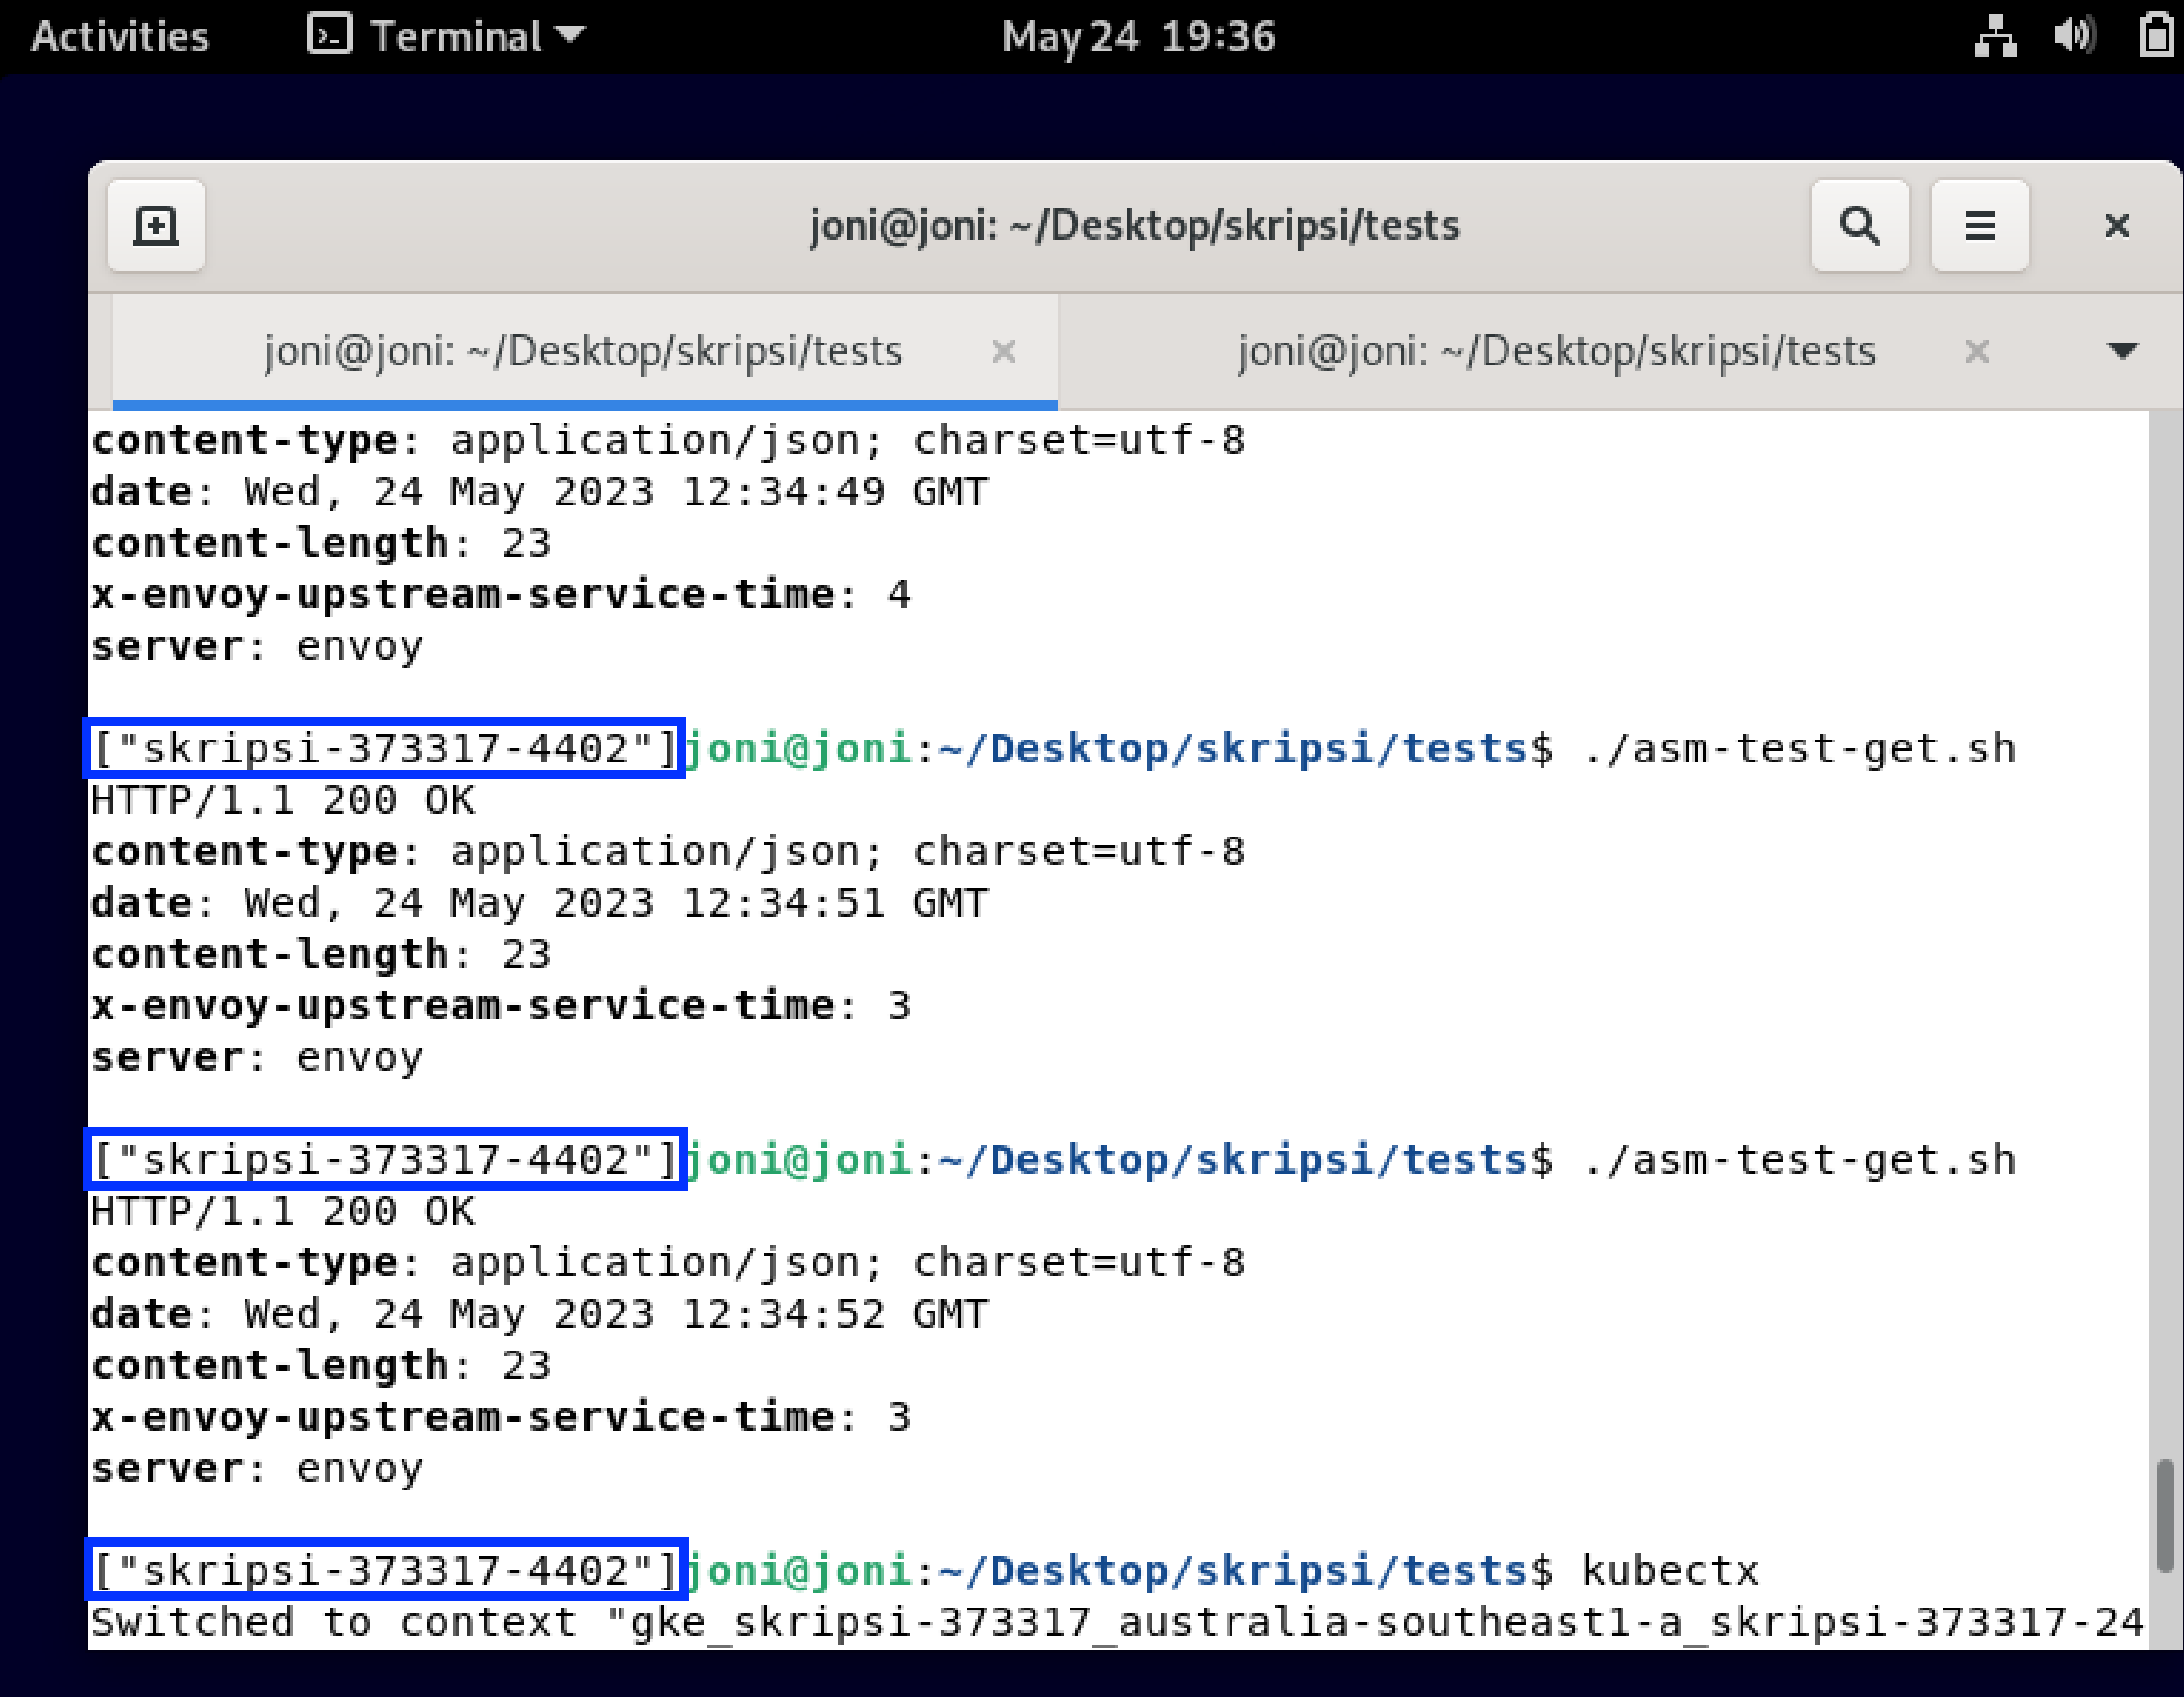
\includegraphics[width=1\textwidth]{assets/pics/5-sea-locality.png}
	\caption{Geo-aware routing from southeast-asia cluster.}
	\label{fig:5-sea-locality}
\end{figure}

\begin{figure}
	\centering
	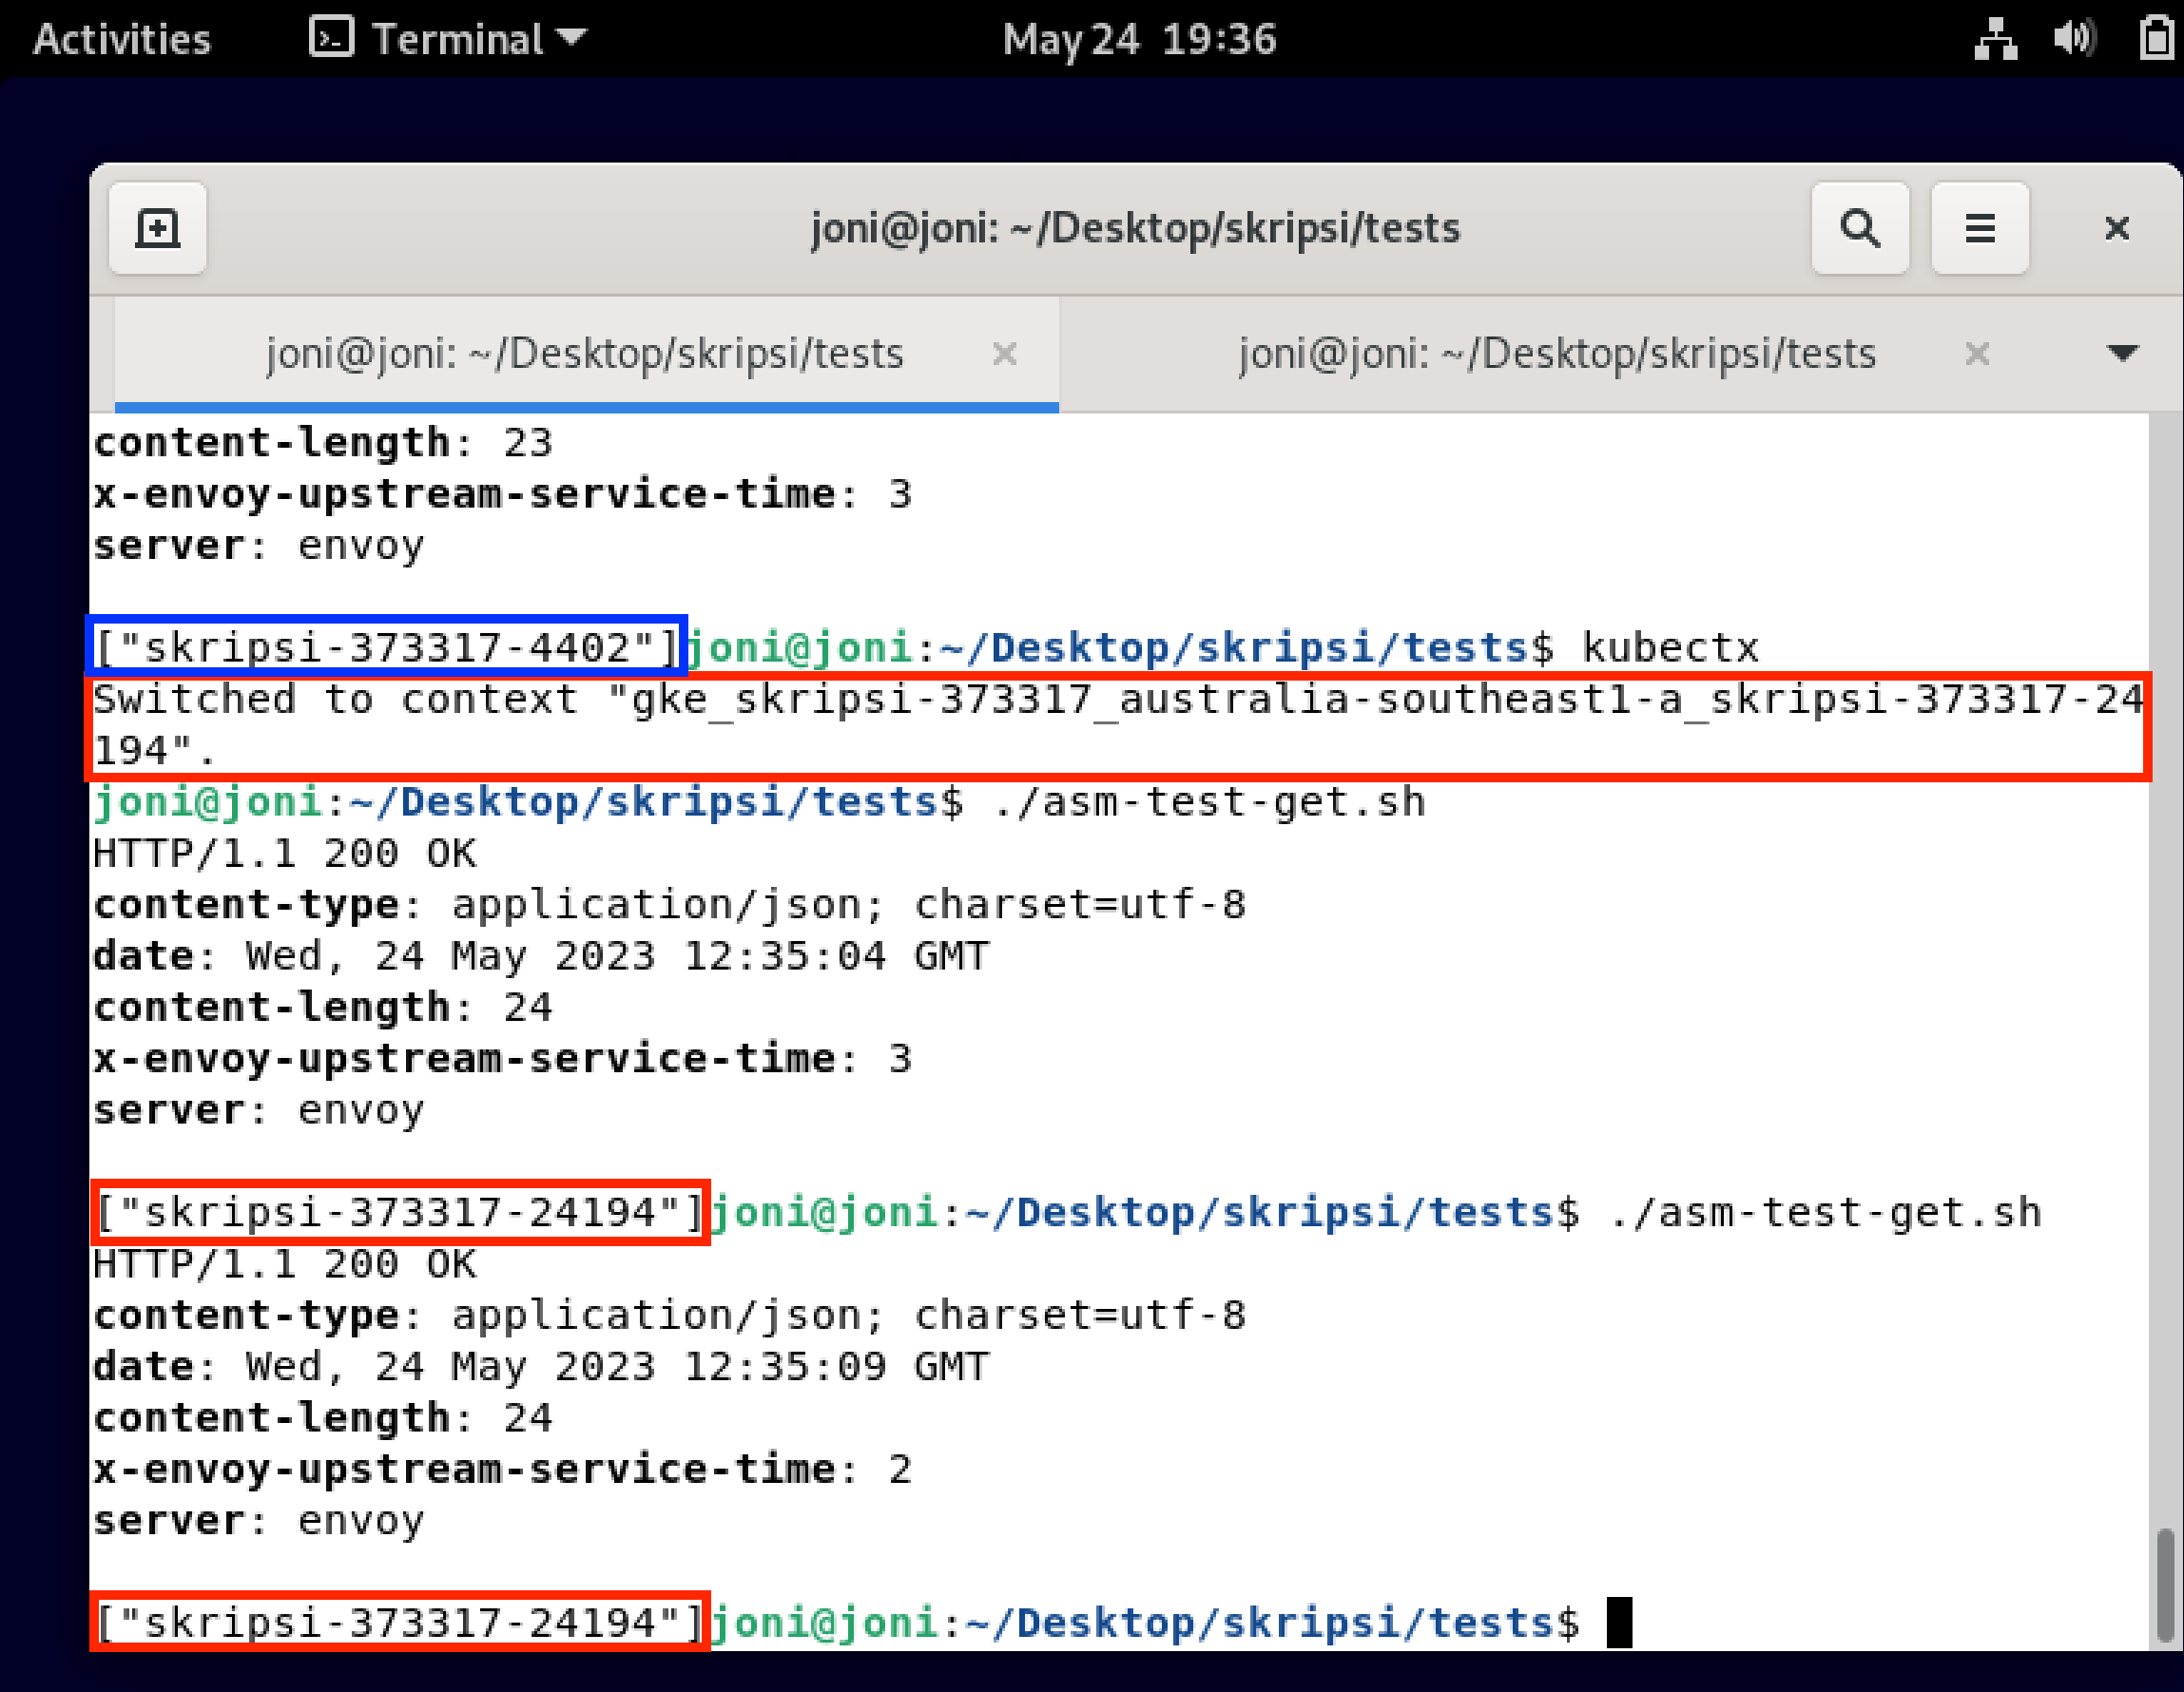
\includegraphics[width=1\textwidth]{assets/pics/5-aus-locality.png}
	\caption{Geo-aware routing from australia cluster.}
	\label{fig:5-aus-locality}
\end{figure}

Furthermore, the results from \autoref{tab:multi-cluster-performance-results} might indicate that MCS with MCI simply outperforms Istio / ASM, as it has a lower mean and lower maximum latency overall. However, it can be seen from \autoref{fig:latency-plot-mc-aus-2} and \autoref{fig:latency-plot-asm-aus-2} that the latency over time of Istio / ASM is comparable to MCI with MCS.

% \begin{table}[h]
% \centering
% \caption{Multi-Cluster Performance Test Results}

% \begin{tabular}{|c|c|c|c|c|c|c|c|}
% \hline


% & & \multicolumn{6}{c|}{\textbf{Latency (ms)}} \\ \cline{3-8}
% \textbf{Location} & \textbf{RPS} & \multicolumn{2}{c|}{\textbf{Min}} & \multicolumn{2}{c|}{\textbf{Mean}}  & \multicolumn{2}{c|}{\textbf{Max}} \\ \cline{3-8}
% &  & \textbf{MCS} & \textbf{ASM} & \textbf{MCS} & \textbf{ASM} & \textbf{MCS} & \textbf{ASM} \\ \hline


% southeast-asia & 10 & \textbf{2.841} & 3.497 & \textbf{3.836} & 35.543 & \textbf{8.219} & 103.985  \\ \cline{3-8}
% southeast-asia & 50 & \textbf{2.487} & 3.594 & \textbf{3.657} & 10.724 & \textbf{8.992} & 103.524  \\ \cline{3-8}
% southeast-asia & 100 & \textbf{2.434} & 3.158 & \textbf{3.96} & 6.52 & \textbf{14.286} & 293.551  \\ \cline{3-8}
% australia & 10 & 3.56 & \textbf{3.509} & 4.723 & \textbf{4.42} & \textbf{8.819} & 58.857 \\ \cline{3-8}
% australia & 50 & 3.261 & \textbf{2.967} & 4.366 & \textbf{3.868} & \textbf{10.318} & 10.506 \\ \cline{3-8}
% australia & 100 & 3.178 & \textbf{2.789} & \textbf{4.097} & 7.735 & \textbf{14.572} & 291.411  \\ \hline

% \end{tabular}
% \label{tab:mean-multi-cluster-results}
% \end{table}

\begin{figure}
	\centering
	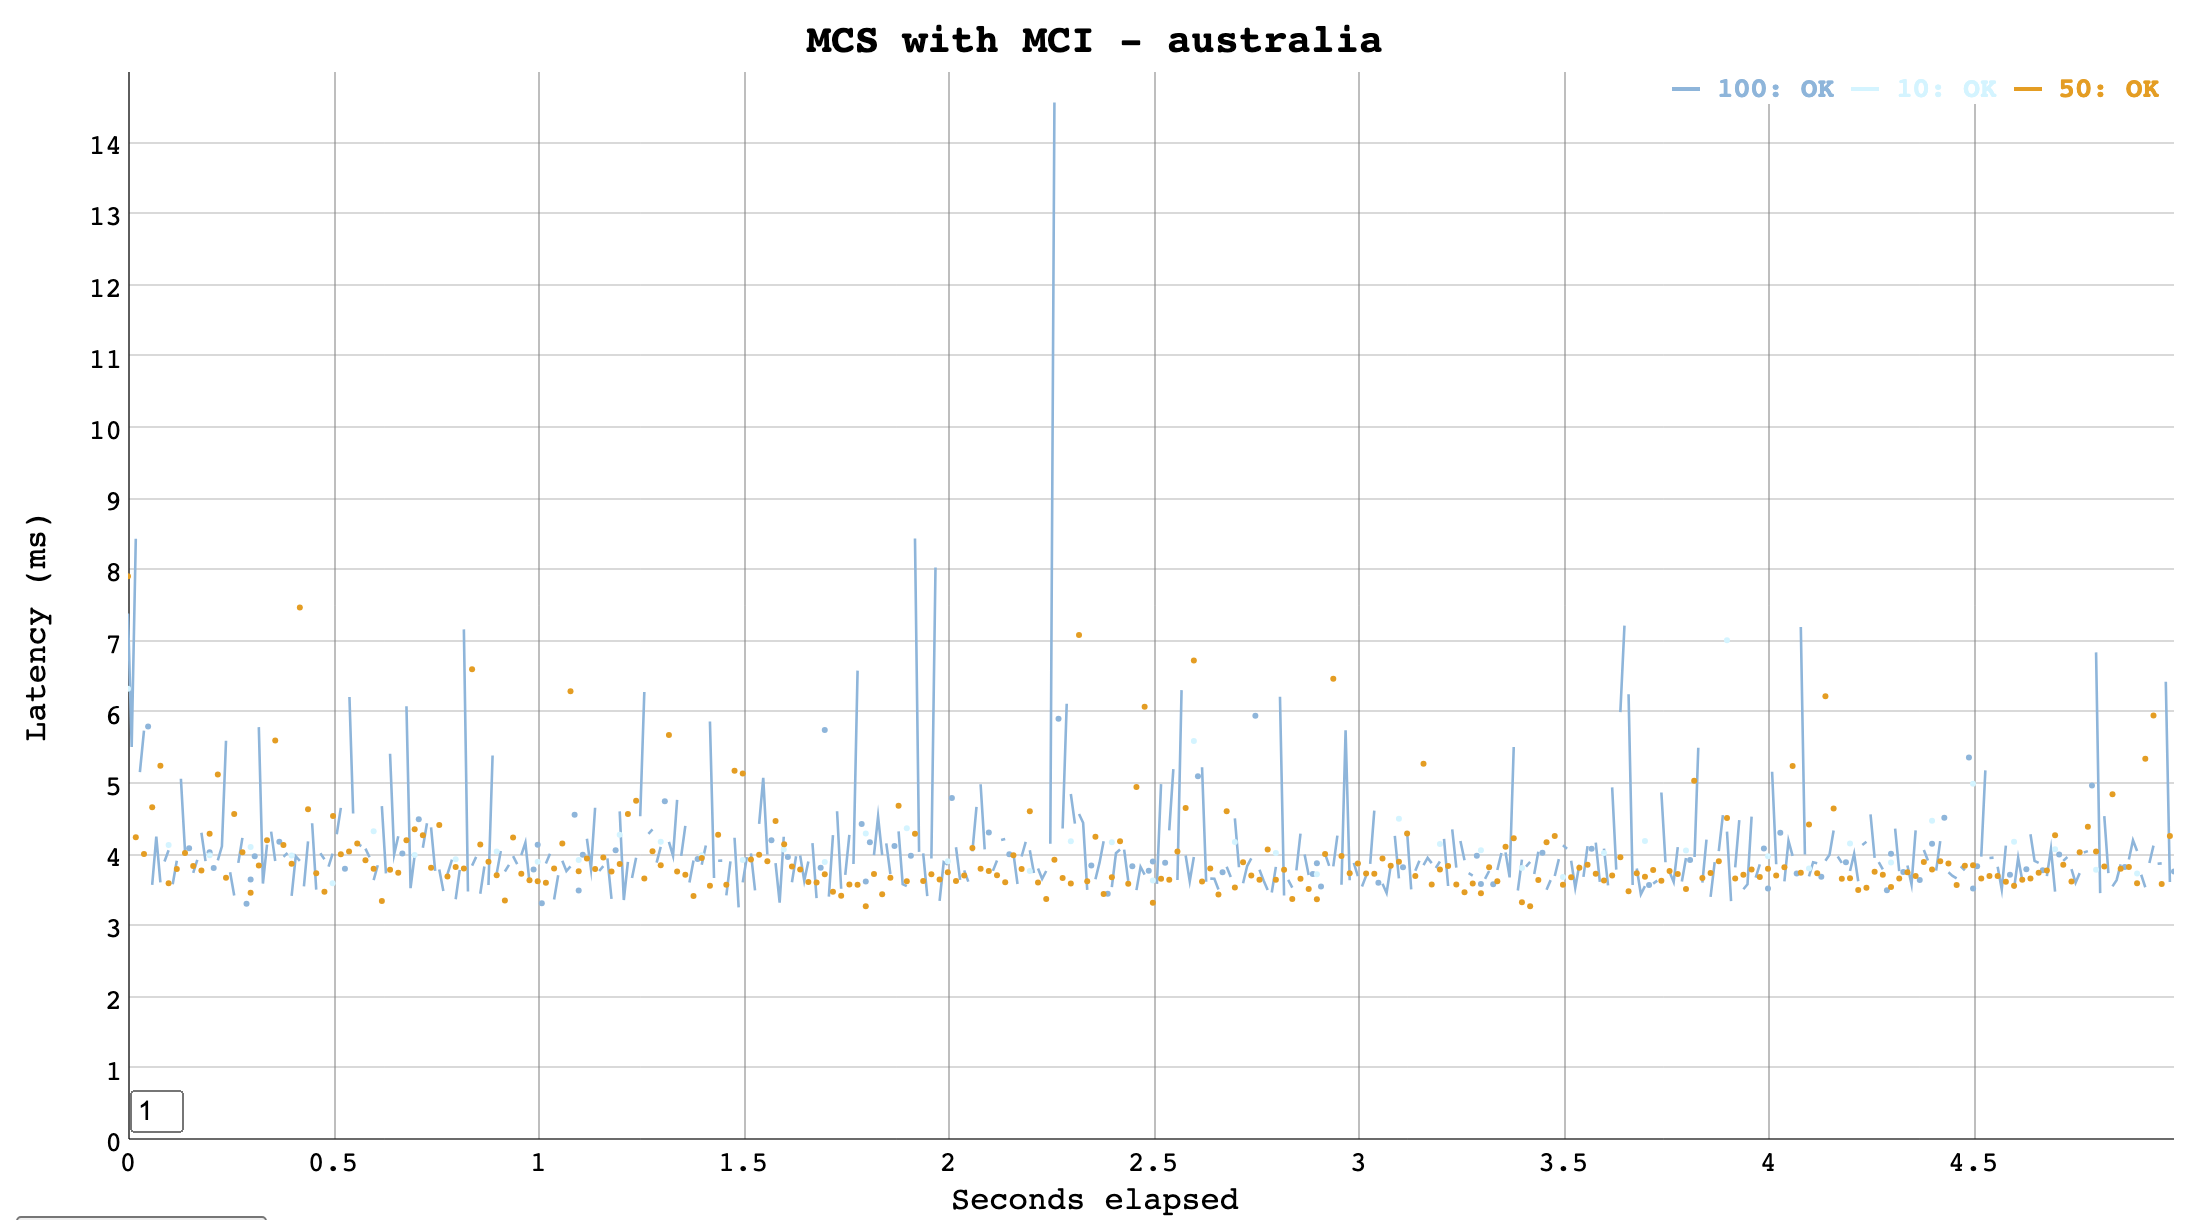
\includegraphics[width=1\textwidth]{assets/plots/mc-aus-2.png}
	\caption{Latency over time of MCS with MCI australia 3.}
	\label{fig:latency-plot-mc-aus-2}
\end{figure}

\begin{figure}
	\centering
	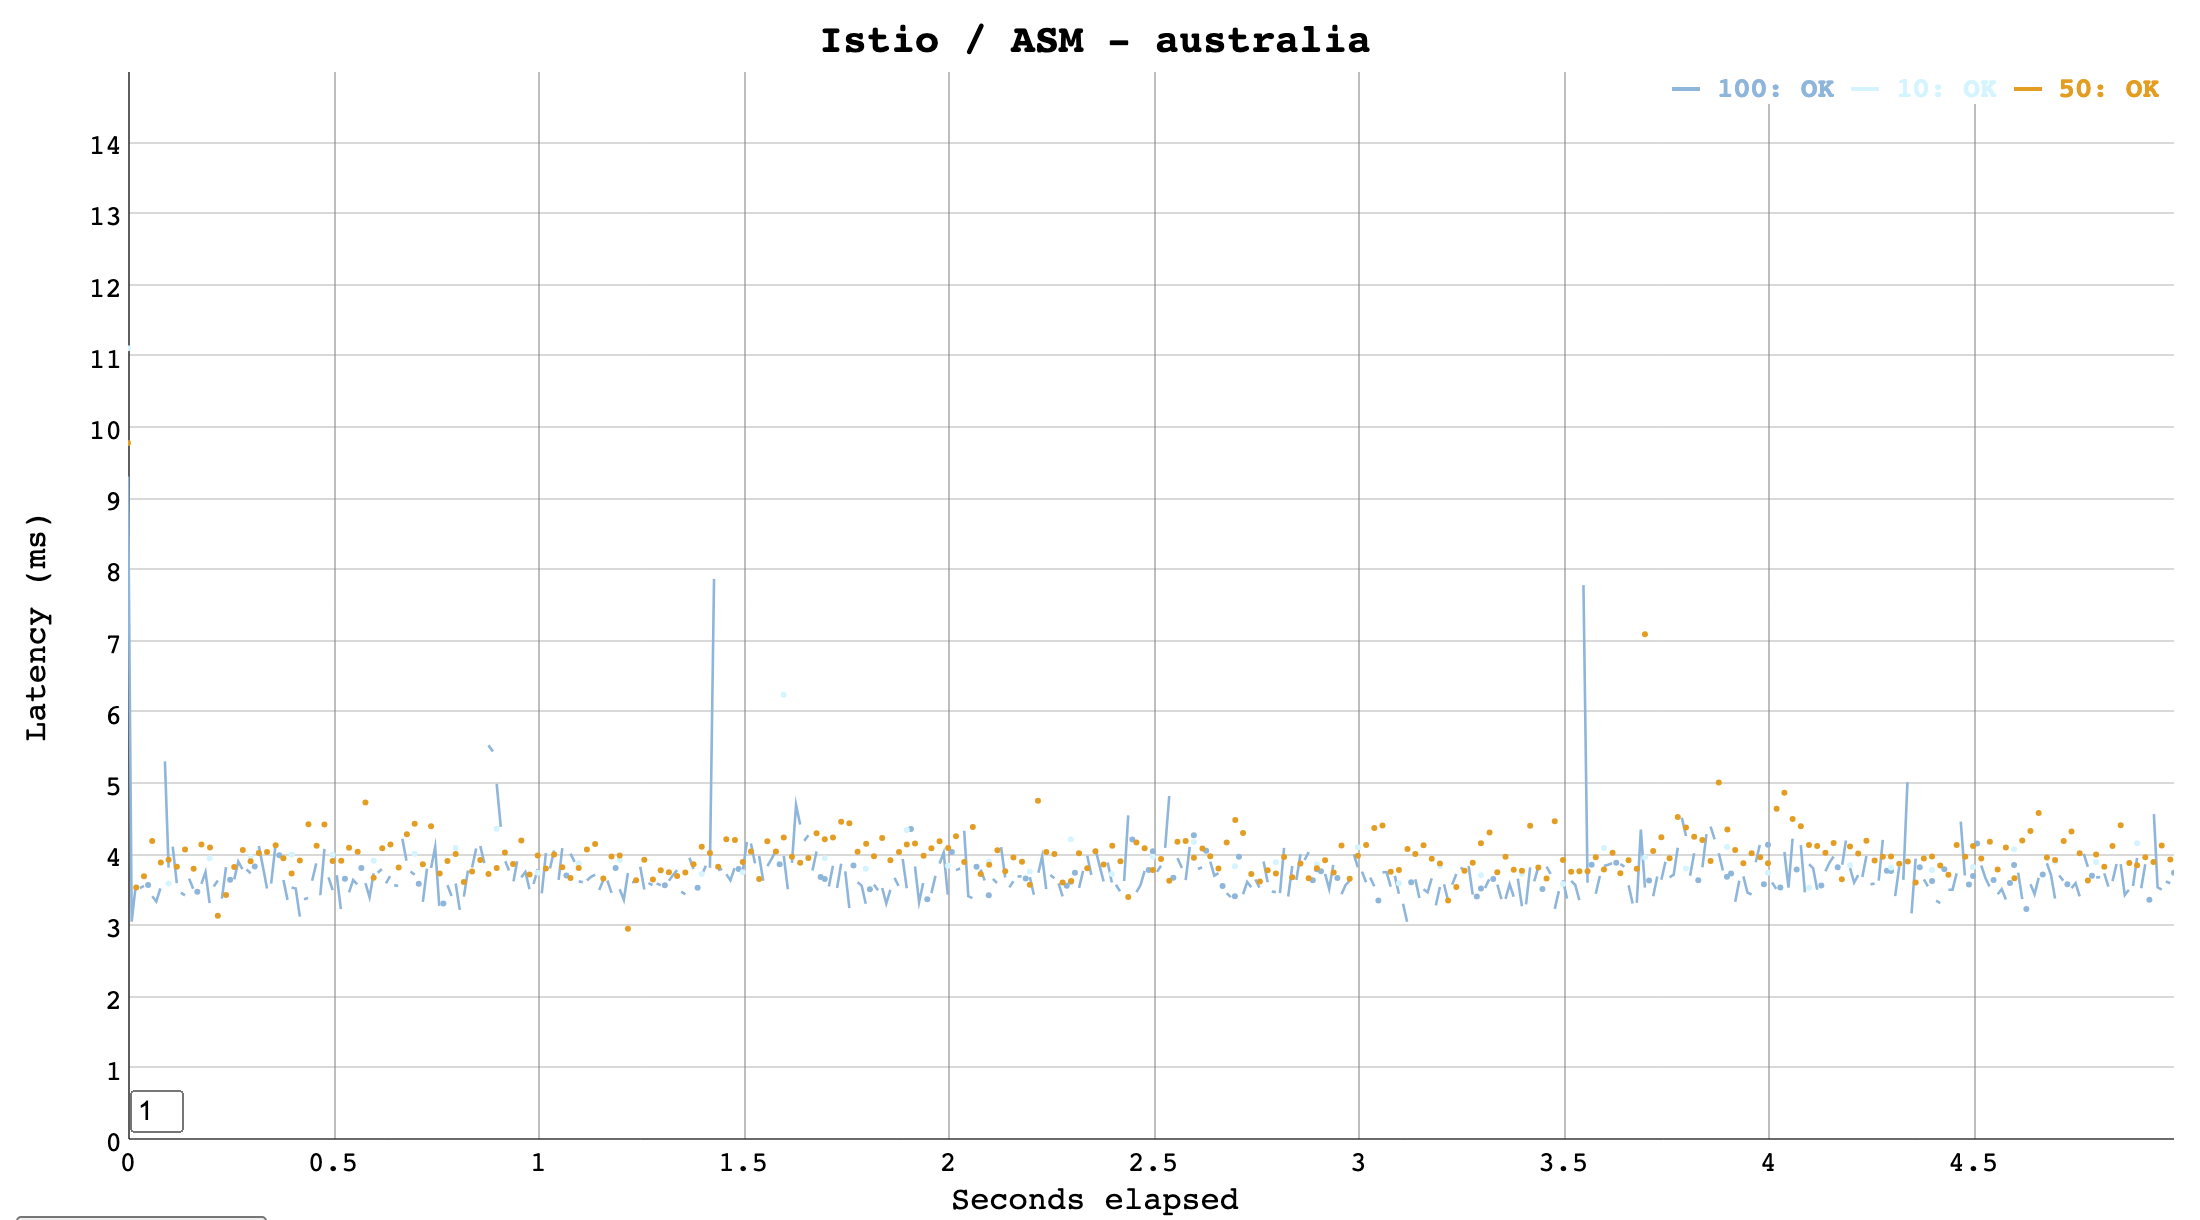
\includegraphics[width=1\textwidth]{assets/plots/asm-aus-2.png}
	\caption{Latency over time of Istio / ASM australia 2.}
	\label{fig:latency-plot-asm-aus-2}
\end{figure}

Further testing shows that the reason Istio / ASM method has a worse overall result is the occurrence of performance outliers, as seen in \autoref{fig:latency-plot-asm-sea-1} and  \autoref{fig:latency-plot-asm-aus-3}, the latency over time for the southeast-asia and australia region, respectively. These outliers produced responses with upwards of 300 milliseconds latency and indicate that the Istio / ASM method is prone to under-performance during high-traffic situations. This can be explained by the slow server recovery time shown in \autoref{tab:reliability-single-cluster-results}, where the failed responses must be redirected to a server with a nonoptimal geographic distance.

\begin{figure}
	\centering
	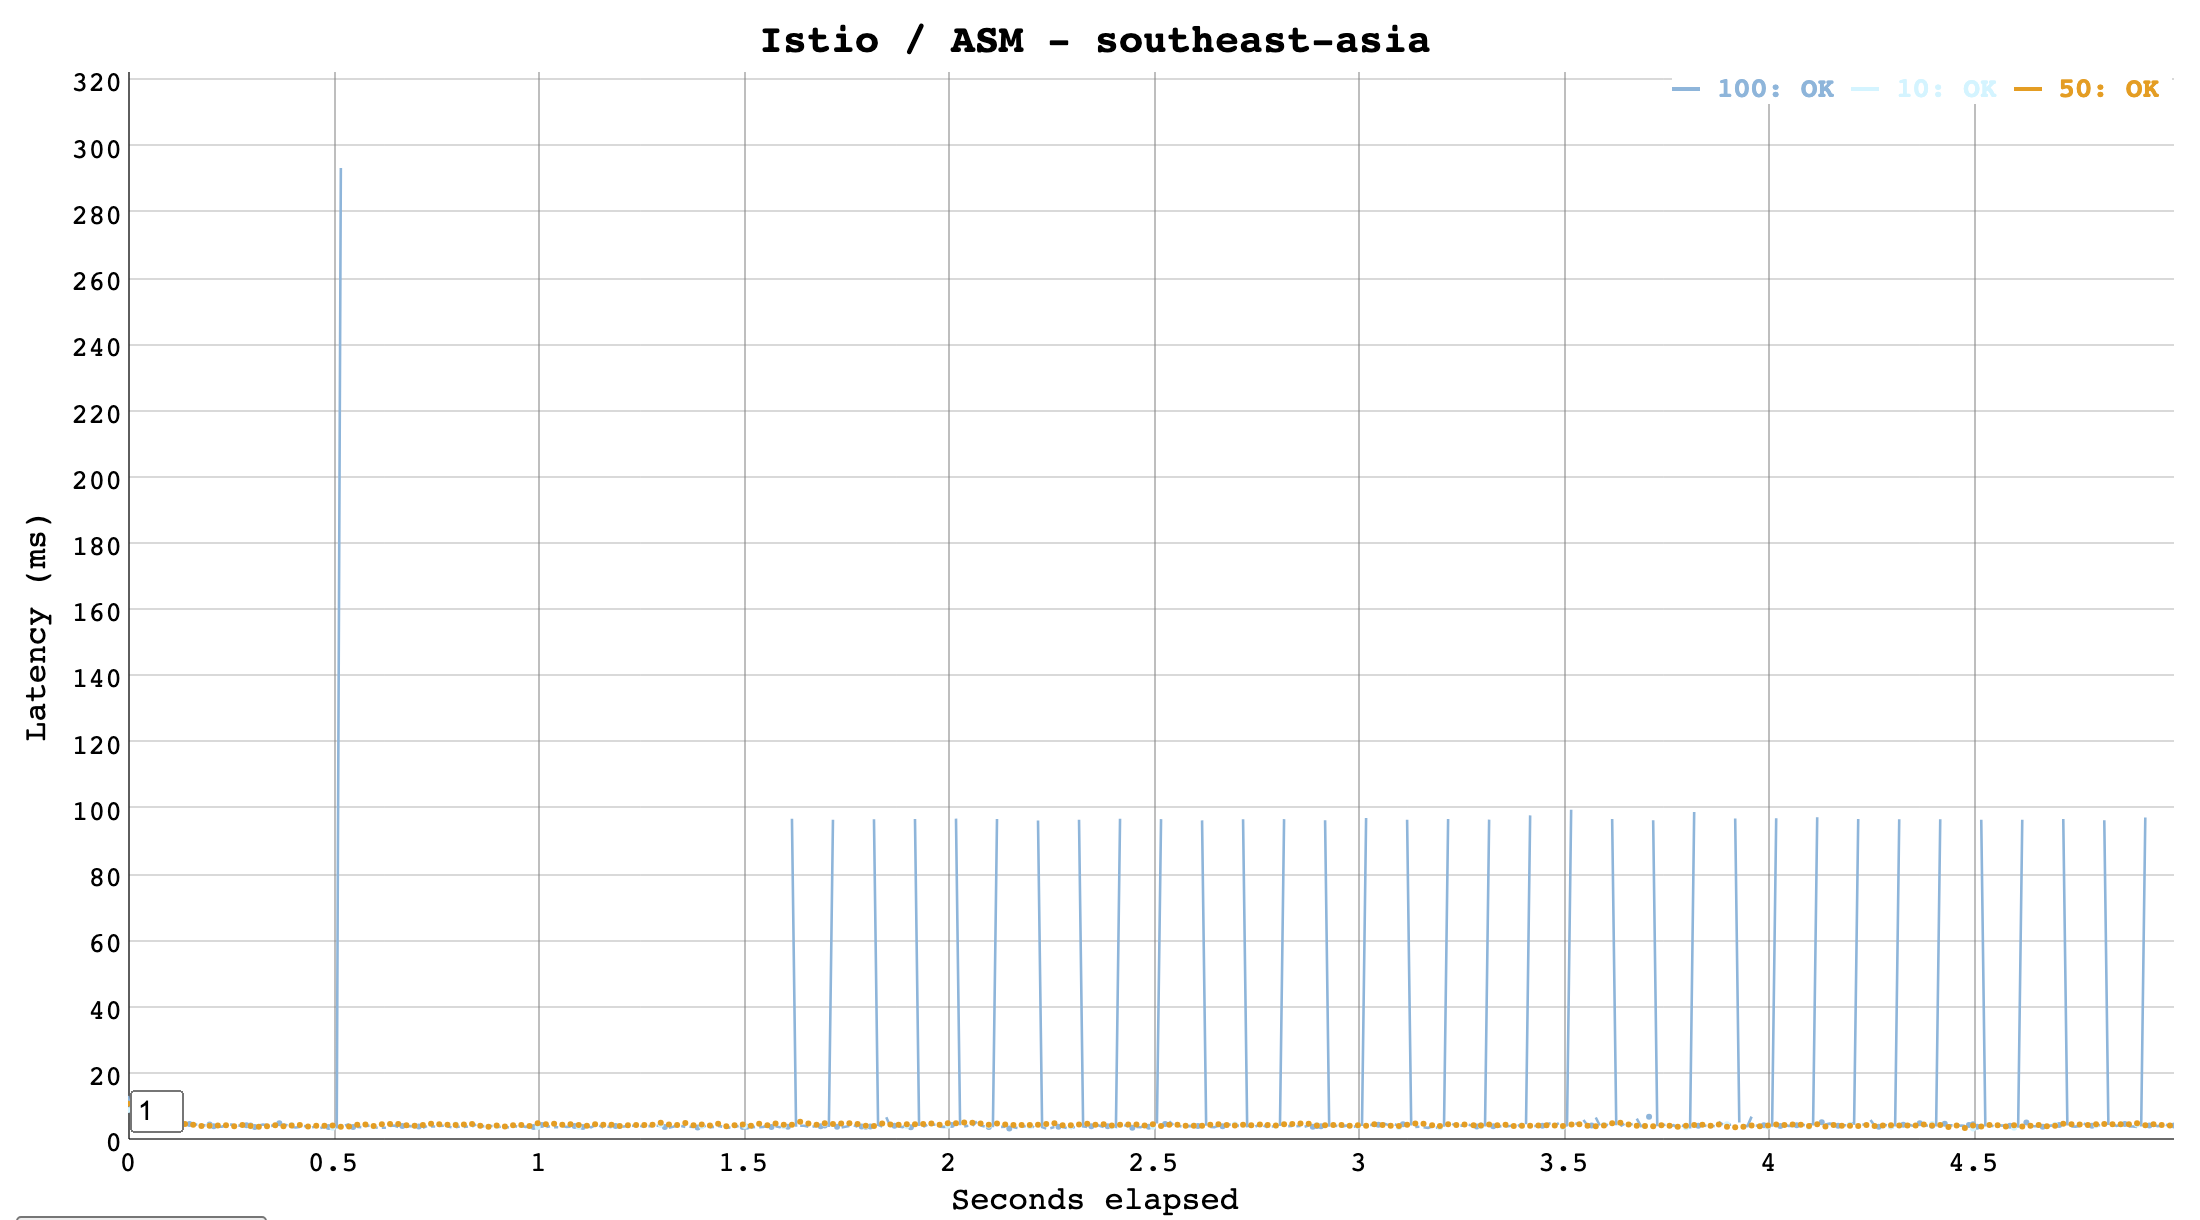
\includegraphics[width=1\textwidth]{assets/plots/asm-sea-1.png}
    \caption{Latency over time of Istio / ASM southeast-asia 1.}
	\label{fig:latency-plot-asm-sea-1}
\end{figure}

\begin{figure}
	\centering
	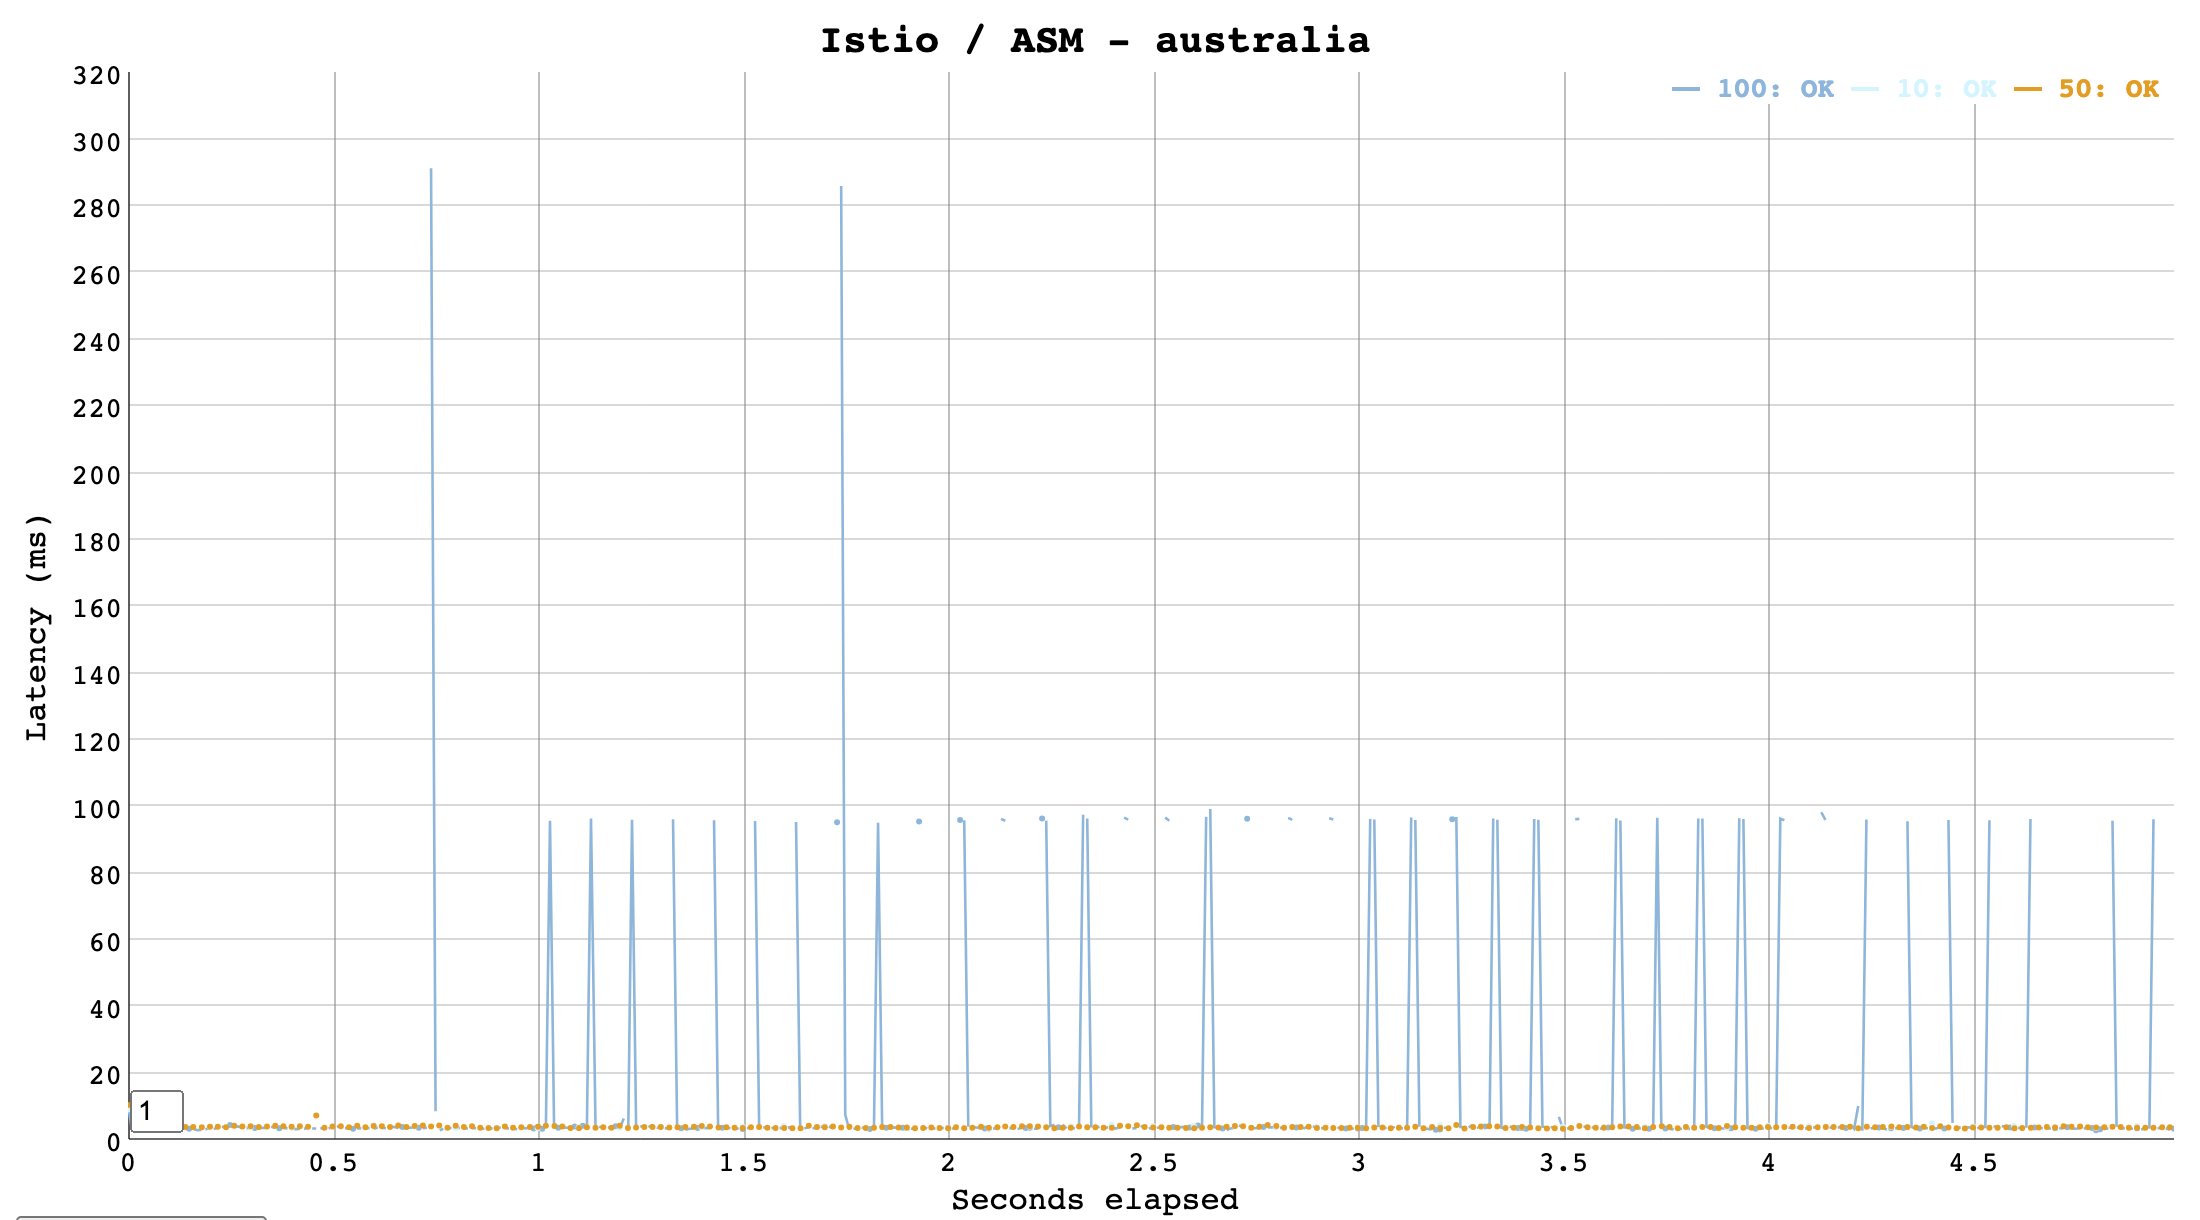
\includegraphics[width=1\textwidth]{assets/plots/asm-aus-3.png}
	\caption{Latency over time of Istio / ASM australia 3.}
	\label{fig:latency-plot-asm-aus-3}
\end{figure}

Conversely, test results from MCS with MCI as seen in \autoref{fig:latency-plot-mc-aus-1} and \autoref{fig:latency-plot-mc-sea-1} show its consistency as it is able to maintain its performance through multiple experiments. There hasn't been an occurrence where MCS with MCI takes longer than 15 milliseconds to respond. This can be explained by MCS with MCI's excellent single-cluster performance, as its server is able to recover from failure in a short amount of time. Furthermore, a single-cluster MCS with MCI outperforms a multi-cluster Istio / ASM configuration in overall latency with an equivalently flawless success ratio.

\begin{figure}
	\centering
	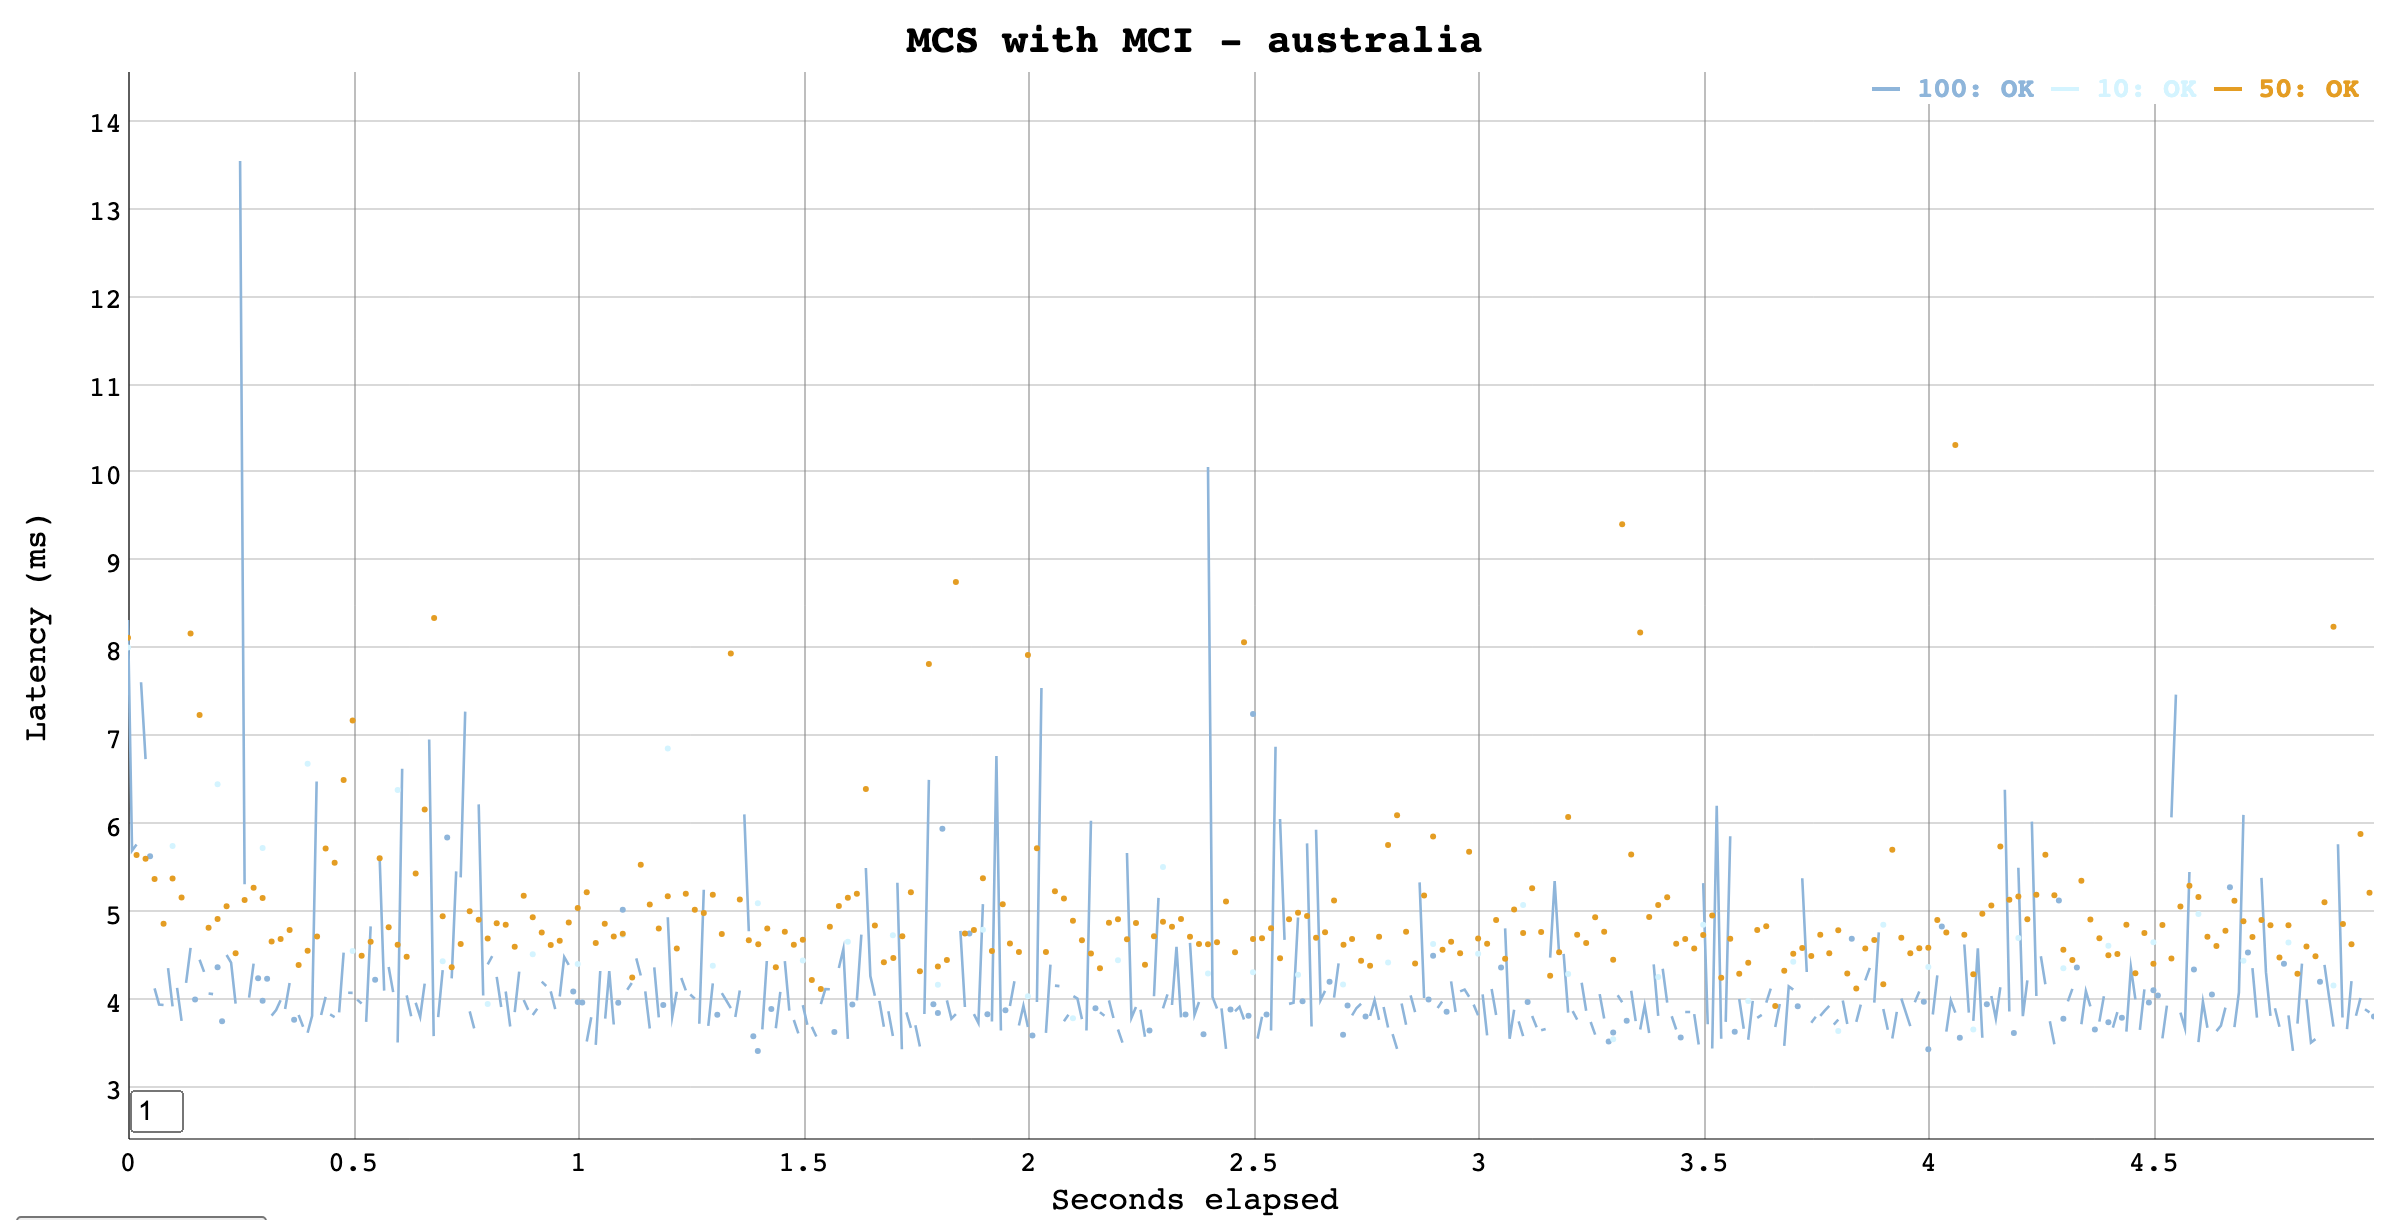
\includegraphics[width=1\textwidth]{assets/plots/mc-aus-1.png}
    \caption{Latency over time of MCS with MCI australia 1.}
	\label{fig:latency-plot-mc-aus-1}
\end{figure}

\begin{figure}
	\centering
	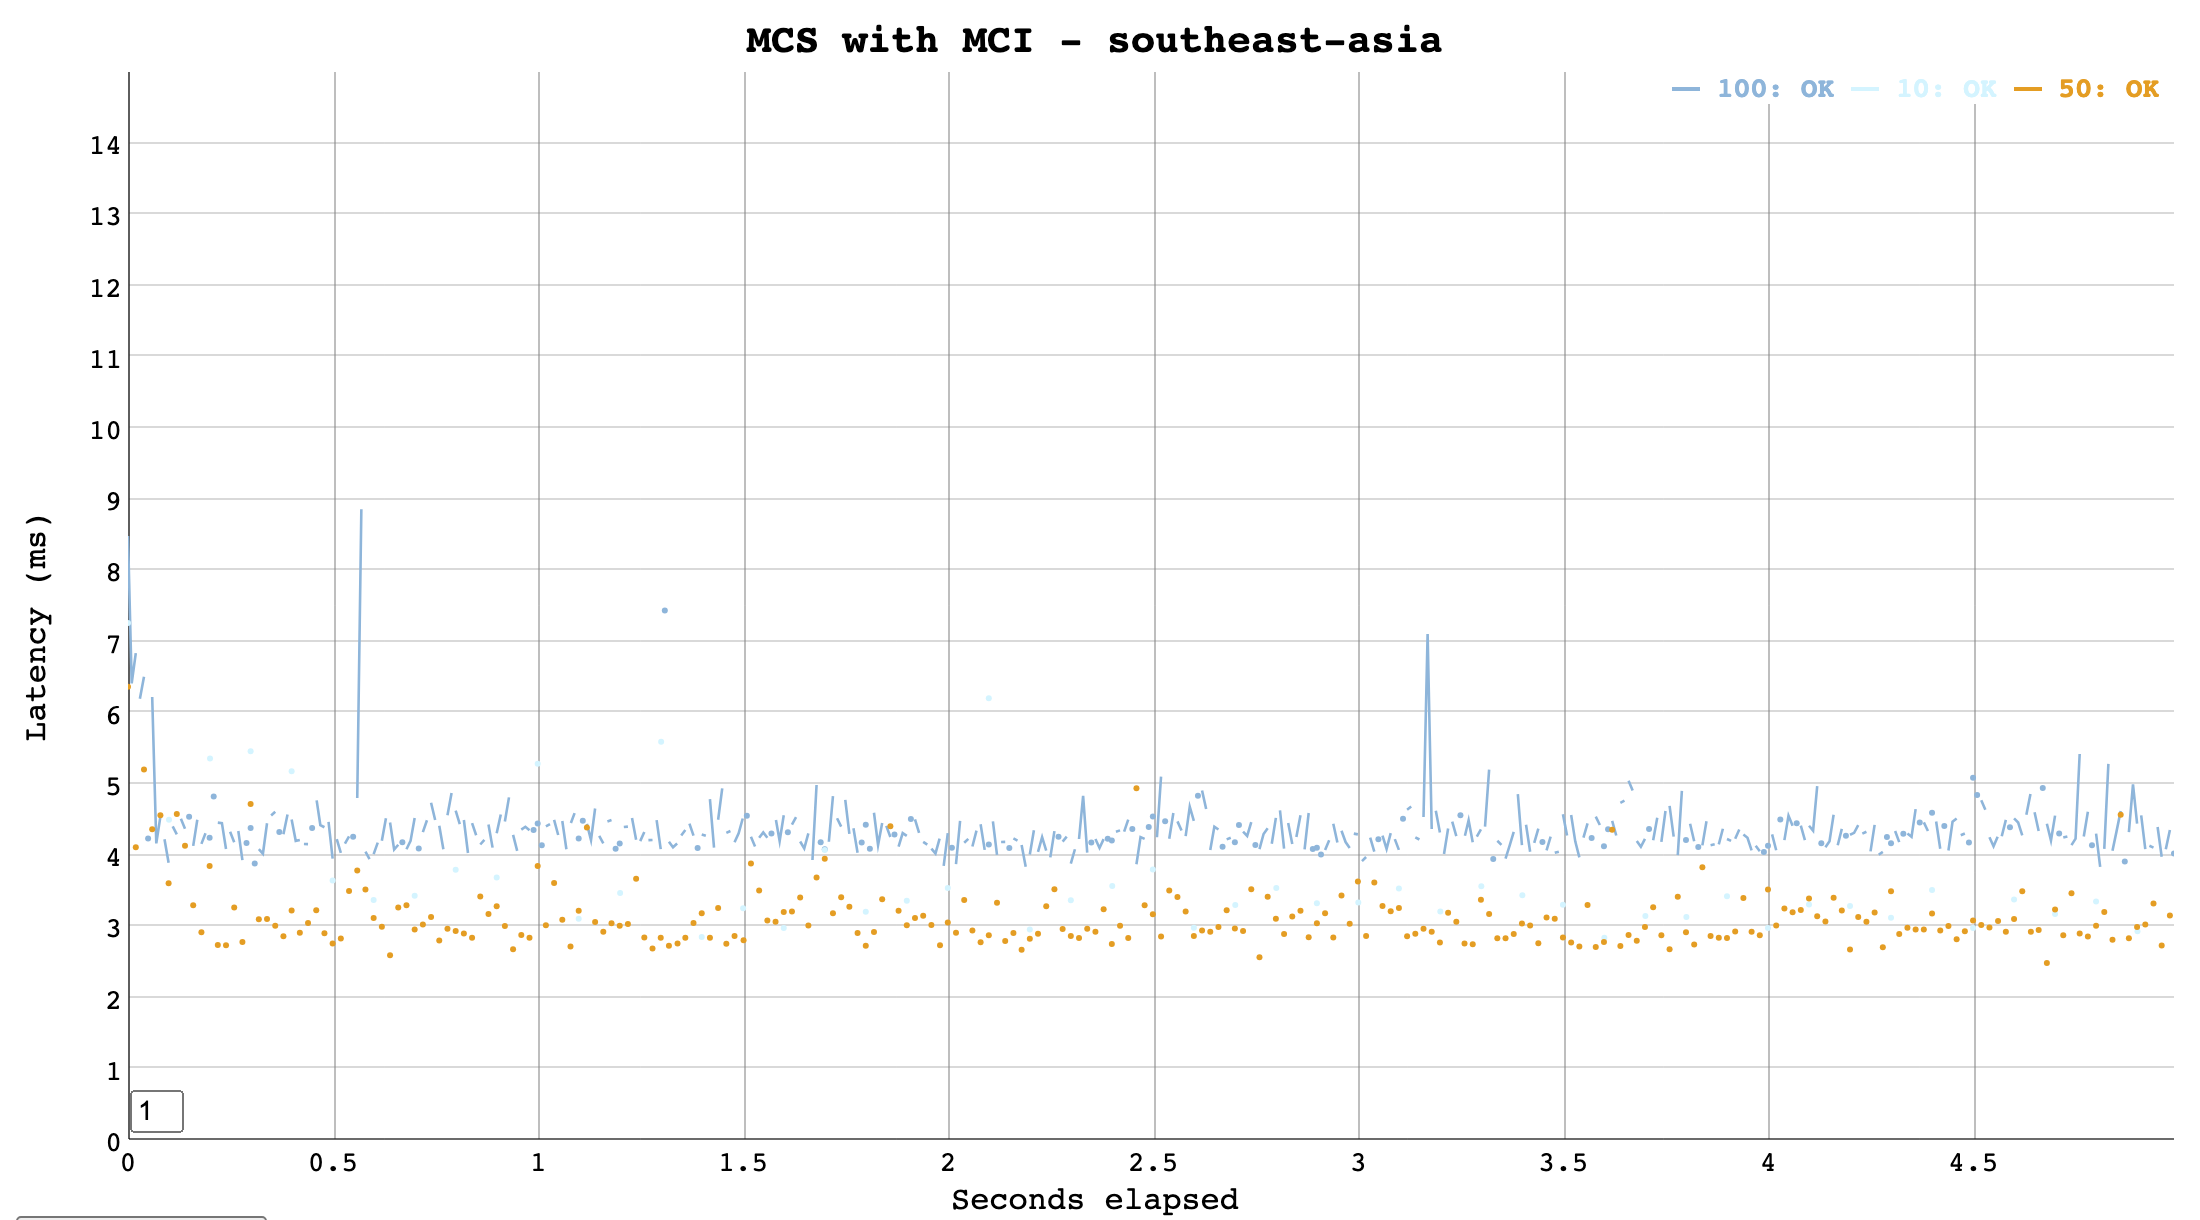
\includegraphics[width=1\textwidth]{assets/plots/mc-sea-1.png}
	\caption{Latency over time of MCS with MCI southeast-asia 1.}
	\label{fig:latency-plot-mc-sea-1}
\end{figure}


To further compare these two approaches, we can compare their latency percentile distribution in order to draw a conclusion. From \autoref{fig:percentile-asm-aus-1-mc-aus-1} and \autoref{fig:percentile-asm-aus-2-mc-aus-2}, it can be seen that Istio / ASM has a lower latency when comparing their 50th and 95th percentile.

\begin{figure}
	\centering
	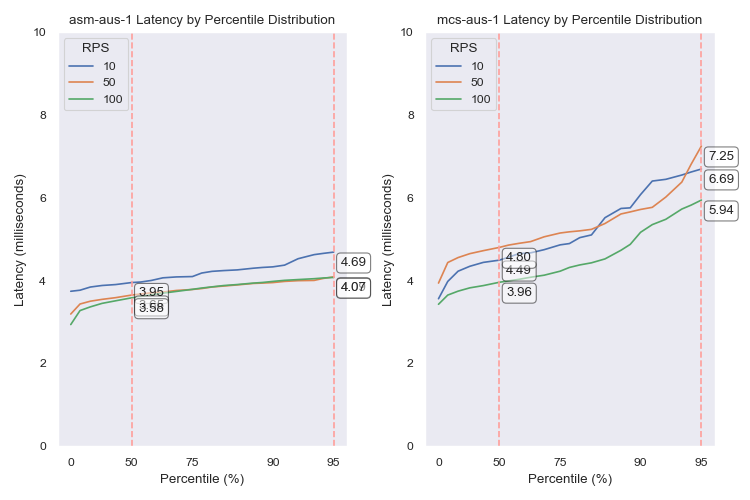
\includegraphics[width=1\textwidth]{assets/plots/percentile-asm-aus-1-mc-aus-1.png}
    \caption{Latency percentile distribution of Istio / ASM and MCS with MCI australia 1.}
	\label{fig:percentile-asm-aus-1-mc-aus-1}
\end{figure}

% \begin{figure}
% 	\centering
% 	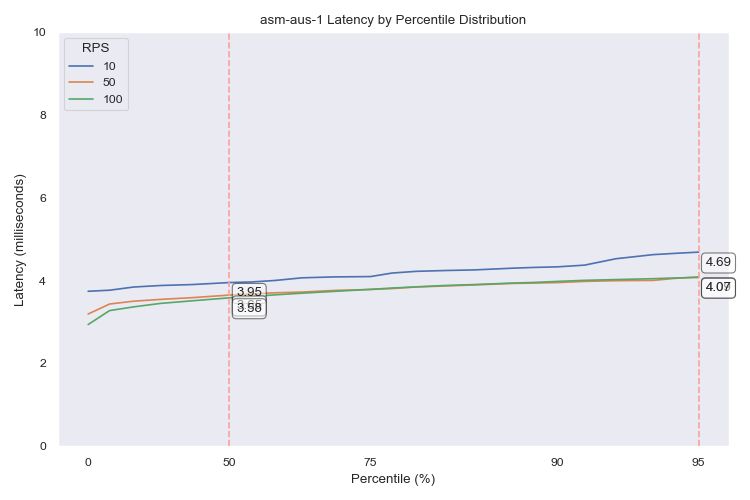
\includegraphics[width=1\textwidth]{assets/plots/percentile-asm-aus-1.png}
%     \caption{Latency percentile distribution of Istio / ASM australia 1.}
% 	\label{fig:percentile-asm-aus-1}
% \end{figure}

% \begin{figure}
% 	\centering
% 	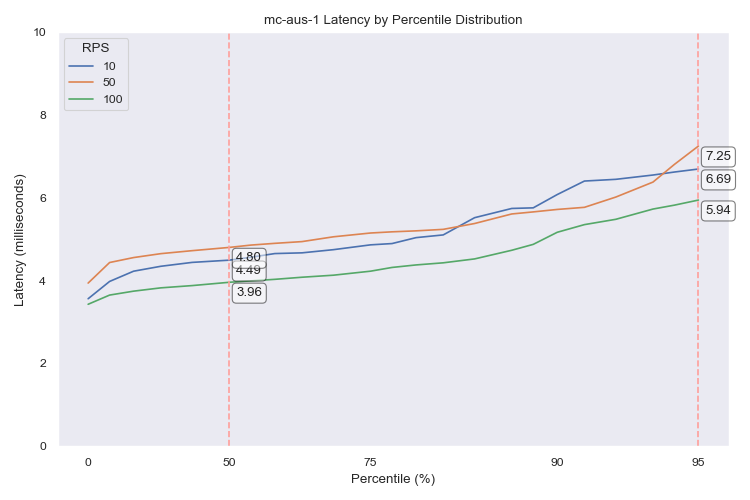
\includegraphics[width=1\textwidth]{assets/plots/percentile-mc-aus-1.png}
% 	\caption{Latency percentile distribution of MCS with MCI australia 1.}
% 	\label{fig:percentile-mc-aus-1}
% \end{figure}

\begin{figure}
	\centering
	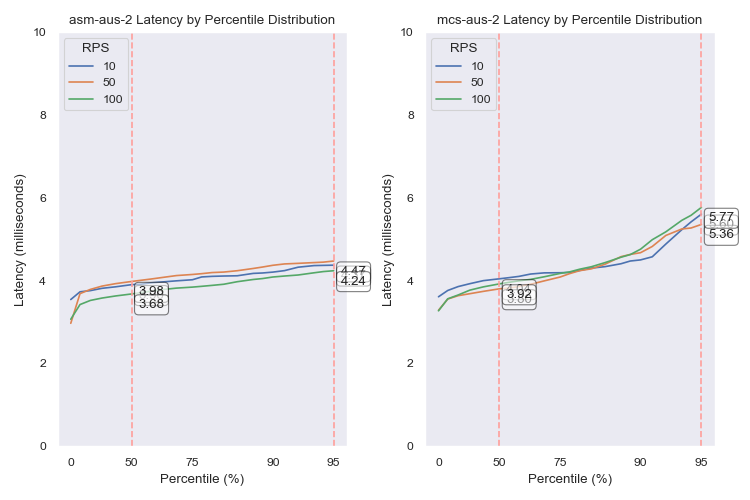
\includegraphics[width=1\textwidth]{assets/plots/percentile-asm-aus-2-mc-aus-2.png}
    \caption{Latency percentile distribution of Istio / ASM and MCS with MCI australia 2.}
	\label{fig:percentile-asm-aus-2-mc-aus-2}
\end{figure}

% \begin{figure}
% 	\centering
% 	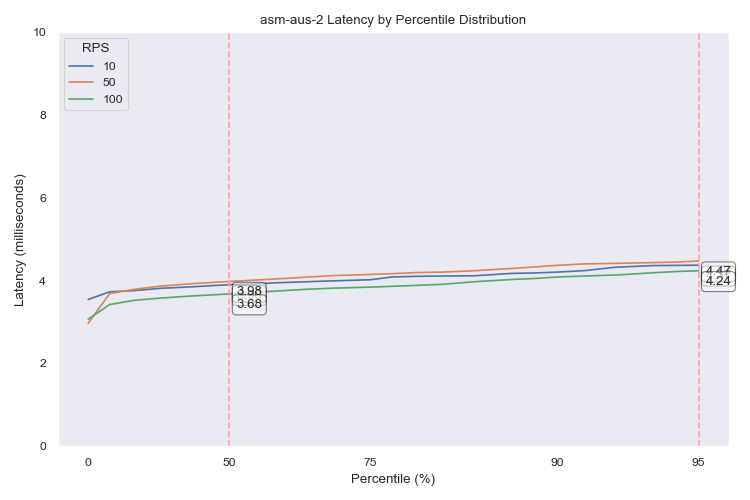
\includegraphics[width=1\textwidth]{assets/plots/percentile-asm-aus-2.png}
%     \caption{Latency percentile distribution of Istio / ASM australia 2.}
% 	\label{fig:percentile-asm-aus-2}
% \end{figure}

% \begin{figure}
% 	\centering
% 	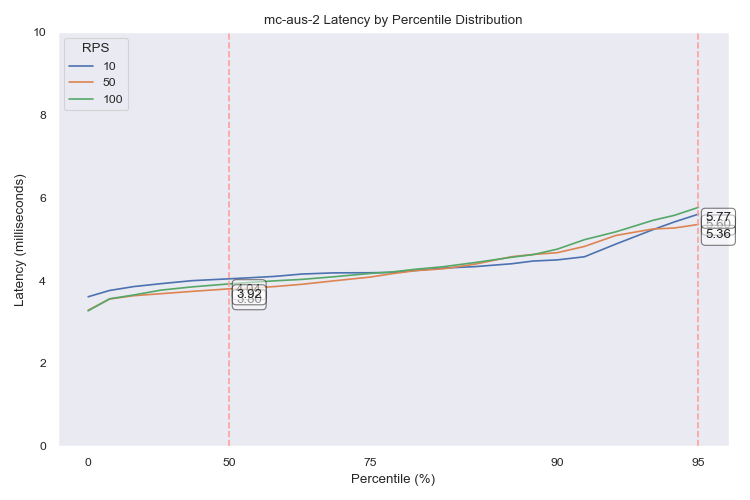
\includegraphics[width=1\textwidth]{assets/plots/percentile-mc-aus-2.png}
% 	\caption{Latency percentile distribution of MCS with MCI australia 2.}
% 	\label{fig:percentile-mc-aus-2}
% \end{figure}

The same result can be seen in the southeast region, where comparing \autoref{fig:percentile-asm-sea-3-mc-sea-3} shows that Istio / ASM has a lower overall latency. We compare the 50th percentile (median) as it is useful to represent what the majority of the response latency looks like. On the other hand, the lower 95th latency percentile and an overall more stable increase compared to the 50th percentile in Istio / ASM tell us that even the small extreme-end of responses that performed worse than normal is still within an acceptable latency.

\begin{figure}
	\centering
	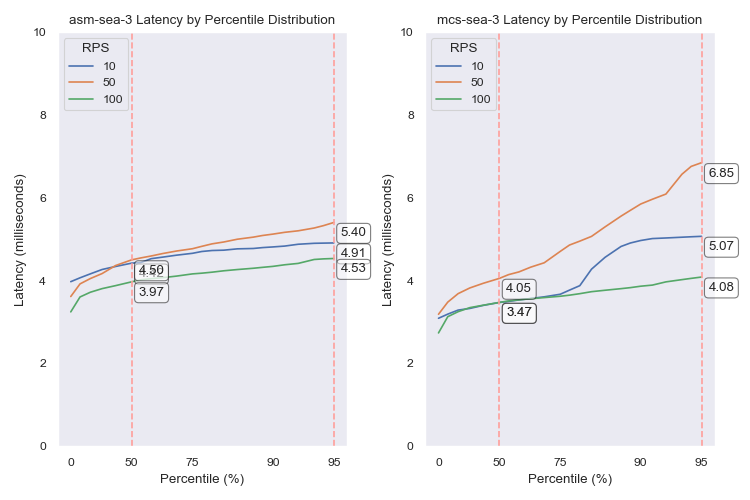
\includegraphics[width=1\textwidth]{assets/plots/percentile-asm-sea-3-mc-sea-3.png}
    \caption{Latency percentile distribution of Istio / ASM and MCS with MCI southeast-asia 3.}
	\label{fig:percentile-asm-sea-3-mc-sea-3}
\end{figure}

% \begin{figure}
% 	\centering
% 	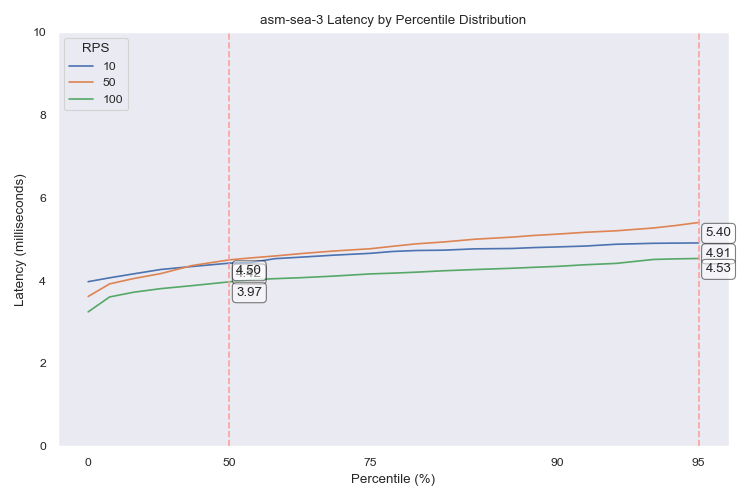
\includegraphics[width=1\textwidth]{assets/plots/percentile-asm-sea-3.png}
%     \caption{Latency percentile distribution of Istio / ASM southeast-asia 3.}
% 	\label{fig:percentile-asm-sea-3}
% \end{figure}

% \begin{figure}
% 	\centering
% 	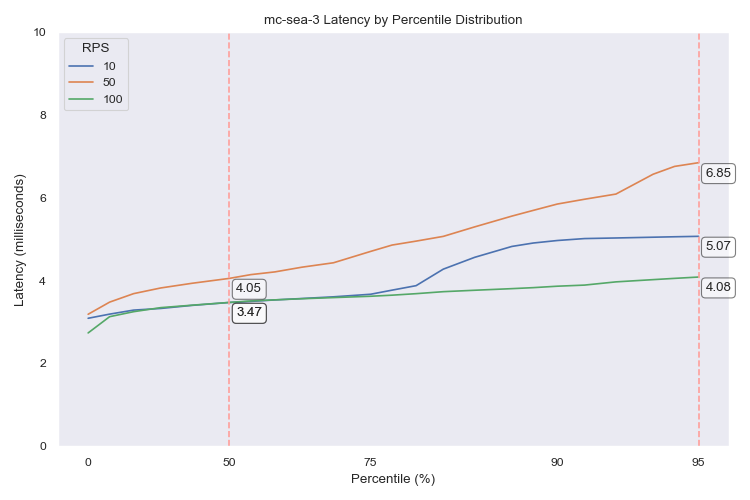
\includegraphics[width=1\textwidth]{assets/plots/percentile-mc-sea-3.png}
% 	\caption{Latency percentile distribution of MCS with MCI southeast-asia 3.}
% 	\label{fig:percentile-mc-sea-3}
% \end{figure}

However, it can't be denied that Istio / ASM suffers from its occasional under-performance, as seen in \autoref{fig:percentile-asm-sea-1-asm-aus-3}, where the jump from the 50th percentile latency to the 95th percentile latency is enormous. This appears to be caused by a combination of  Istio / ASM's slow recovery time and slow failover mechanism, which is not a problem inside an MCS with MCI method.

\begin{figure}
	\centering
	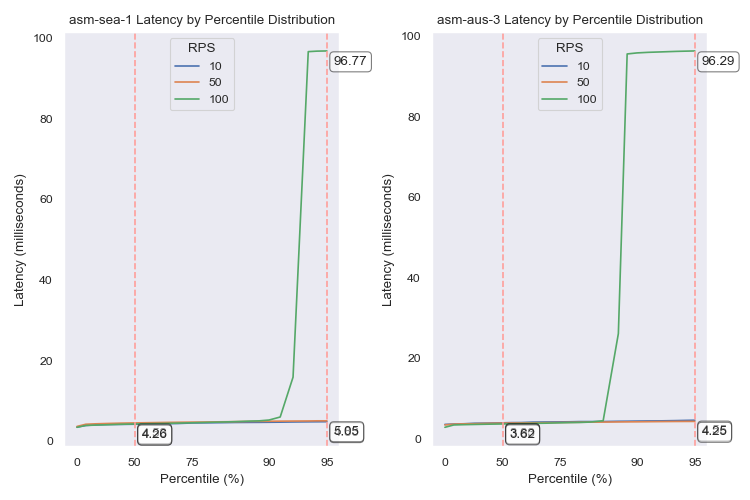
\includegraphics[width=1\textwidth]{assets/plots/percentile-asm-sea-1-asm-aus-3.png}
    \caption{Latency percentile distribution of Istio / ASM southeast-asia 1 and Istio / ASM australia 3.}
	\label{fig:percentile-asm-sea-1-asm-aus-3}
\end{figure}

% \begin{figure}
% 	\centering
% 	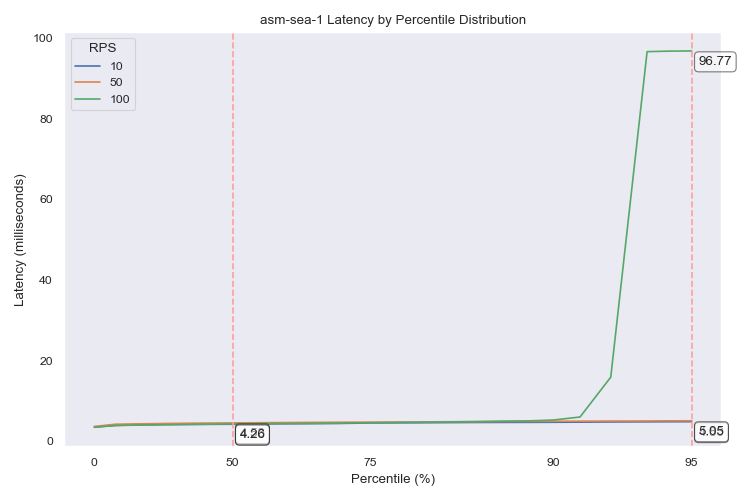
\includegraphics[width=1\textwidth]{assets/plots/percentile-asm-sea-1.png}
%     \caption{Latency percentile distribution of Istio / ASM southeast-asia 1.}
% 	\label{fig:percentile-asm-aus-3}
% \end{figure}

% \begin{figure}
% 	\centering
% 	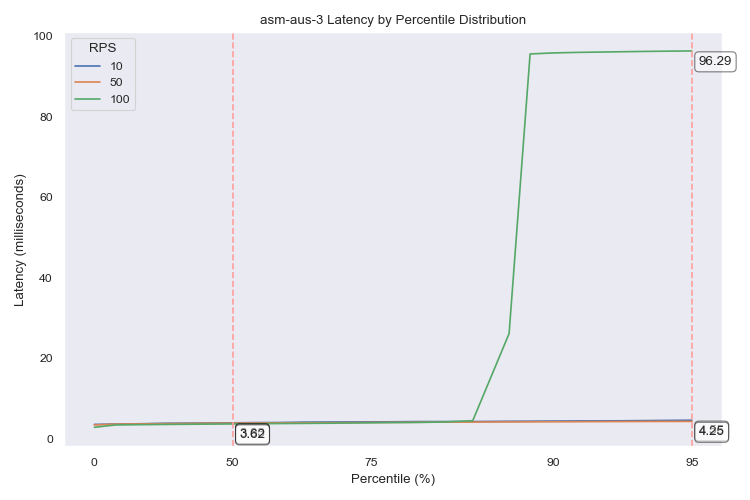
\includegraphics[width=1\textwidth]{assets/plots/percentile-asm-aus-3.png}
% 	\caption{Latency percentile distribution of Istio / ASM australia 3.}
% 	\label{fig:percentile-mc-aus-3}
% \end{figure}

Moreover, comparing the latency's 50th and 90th percentile, as seen in \autoref{tab:multi-cluster-performance-results}, shows that Istio / ASM has the better overall latency, as it has a lower 95th percentile latency in 12 out of 18 experiments with a 1.4-millisecond difference on average compared to the MCS with MCI approach. The MCS with MCI approach has the advantage in 50th percentile performance, however, as it outperforms Istio / ASM 10 out of 18 times with a 10-millisecond difference on average.
% As a result of having a lower 95th percentile latency, Istio / ASM has the better performance. his means that the Istio / ASM approach has a better performance, it is not a significant improvement.


% \clearpage

% Overall, it is true that MCS with MCI has better performance and is a more suitable method for high-traffic scenarios as it consistently handles requests with low-latency responses. This is not to say that Istio / ASM is an objectively worse approach, as it has a diverse amount of features that MCS with MCI doesn't have, such as canary release and rate limiting.

In conclusion, Istio / ASM performs better than MCS with MCI as it is able to handle a wider number of requests with slightly lower latency, despite its outliers. It is advisable to have multiple replicas of each server to avoid long recovery times. Despite this, the difference in median latency is negligible, making MCS with MCI a viable alternative. In addition, an improvement to the failure mechanism can be done by having more clusters to reduce the physical distance between a cluster and its failover destination.

Additionally, it can be seen from \autoref{tab:multi-cluster-performance-results} that Istio / ASM has a lower latency in the australia region while the same can be said with the MCS with MCI method on the southeast-asia region. This is possibly the effect of timezone differences, as the tests were done one after another, which results in different actual local time for each of the region.
\clearchapter
%---------------------------------------------------------------
\chapter{\kesimpulan}
\label{bab:6}
%---------------------------------------------------------------
% Pada bab ini, Penulis akan memaparkan kesimpulan penelitian dan saran untuk penelitian berikutnya.
This chapter discusses the conclusions that resulted from the research conducted, which answers . In addition, this chapter also gives suggestions to further this research.


%---------------------------------------------------------------
\section{Conclusion}
\label{sec:kesimpulan}
%---------------------------------------------------------------
% This research has the following conclusions:

From this research, there are several conclusions that can be made. First of all, the geo-distributed Kubernetes clusters architecture improves the reliability of worldwide applications. Experiment results show that both MCS with MCI and Istio / ASM methods reliably perform at 100\% success rate, making either one a viable choice for application reliabilty. For limited resources, however, MCS with MCI shows better reliability keeping its flawless success rate even with just a single cluster deployed. It is advisable to use the Istio / ASM method with multiple clusters deployed to take advantage if its failover mechanism, as it suffers from slow recovery time, which appears to be the bottleneck for single-cluster reliability.

In addition, Istio / ASM improves application performance. Both MCS with MCI and Istio / ASM methods correctly and efficiently route requests to the cluster with minimal physical distance, which minimizes the overall latency. However, it appears that Istio / ASM is the better choice for application performance as it outperforms MCS with MCI in the 95th percentile of latency on most experiments, which means that its a much more predictable performance, as it is able to deliver lower latency to the vast majority of requests. Despite this, Istio / ASM suffers from outlier performances due to its slow recover and failover time.

% \begin{enumerate}
% 	\item \bo{Multi-cluster load balancing improves the reliability of worldwide applications} \\
% 	Experiment results show that both MCS with MCI and Istio / ASM methods reliably perform at 100\% success rate, making either one a viable choice for application reliabilty. For limited resources, however, MCS with MCI shows better reliability keeping its flawless success rate even with just a single cluster deployed. It is advisable to use the Istio / ASM method with multiple clusters deployed to take advantage if its failover mechanism, as it suffers from slow recovery time, which appears to be the bottleneck for single-cluster reliability.
% 	\item \bo{Istio improves the performance of worldwide application} \\
% 	Both MCS with MCI and Istio / ASM methods correctly and efficiently route requests to the cluster with minimal physical distance, which minimizes the overall latency. However, it appears that Istio / ASM is the better choice for application performance as it outperforms MCS with MCI in the 95th percentile of latency on most experiments, which means that its a much more predictable performance, as it is able to deliver lower latency to the vast majority of requests. Despite this, Istio / ASM suffers from outlier performances due to its slow recover and failover time.
% \end{enumerate}

% Berikut ini adalah kesimpulan terkait pekerjaan yang dilakukan dalam penelitian ini:
% \begin{enumerate}
% 	\item \bo{Poin pertama} \\
% 	Penjelasan poin pertama.
% 	\item \bo{Poin kedua} \\
% 	Penjelasan poin kedua.
% \end{enumerate}

% Tulis kalimat penutup di sini.
Overall, both geo-distributed methods are viable options for worldwide application usage in terms of both reliability and performance. MCS with MCI has its upsides of consistently performing within normal latency ranges while Istio / ASM has a slightly better performance for the majority of the requests but suffers from latency spikes in small cases.

%---------------------------------------------------------------
\section{Suggestions}
\label{sec:saran}
% %---------------------------------------------------------------
% Berdasarkan hasil penelitian ini, berikut ini adalah saran untuk pengembangan penelitian berikutnya:
% \begin{enumerate}
% 	\item Saran 1.
% 	\item Saran 2.
% \end{enumerate}

From this research, there are several suggestions that can be done in further studies, one of which, is to study the effects of increasing the replicas of each server. Since Istio / ASM adds complexity to a Kubernetes architecture, it would be useful to research about the effects of horizontal scaling on its overall performance. In addition, further research should be done on other cloud platforms as well, as Google Cloud Platform is only one of many other available cloud service providers such as AWS and Azure. Comparisons between different cloud service providers can be useful to share knowledge about prices between providers as well as overall ease of use for the average developer. In addition, a wider variety of cloud services can be used as different client origins to study the effects of intra-cloud and inter-cloud web performance. Furthermore, future researches should also explore different and/or more regions to measure reliability and performance on a wider geographical scale.

In addition, it would be beneficial to do research on other open-sourced service mesh such as Linkerd and Consul to help understand the benefits and drawbacks of each service mesh implementation and its various features. Furthermore, studies on geo-distributed databases should be explored, as it is one of the most important part of a web application. It is, however, a complex topic that introduces geo-distributed partitioning and replica replacement.
 % Moreover, adding a more 
\clearchapter

%
% Daftar Pustaka
\CAPinToC % All entries in ToC will be CAPITALIZED from here on
%
% Daftar Pustaka
%

%
% Tambahkan pustaka yang digunakan setelah perintah berikut.
%
\phantomsection %hack to add clickable section for pustaka
\bibliography{config/references}

\clearchapter
\noCAPinToC % Revert to original \addcontentsline formatting

%
% Lampiran
%
\begin{appendix}
	\newcounter{pagetemp}
	\setcounter{pagetemp}{\thepage}
	%
% @author  Andreas Febrian
% @version 1.00
%
% Hanya sebuah pembatas bertuliskan LAMPIRAN ditengah halaman.
%

\begin{titlepage}
\centering
\vspace*{6cm}
\noindent \Huge{LAMPIRAN}
\end{titlepage}

	\clearchapter
	\setcounter{page}{\thepagetemp}
	\stepcounter{page}
	% %-----------------------------------------------------------------------------%
% \addappendix{CHANGELOG}
% \chapter*{Lampiran 1: CHANGELOG}
% \label{appendix:changelog}
% %-----------------------------------------------------------------------------%
% \todo{Silakan hapus lampiran ini ketika Anda mulai menggunakan \f{template}.}

% \f{Template} versi terbaru bisa didapatkan di \url{https://gitlab.com/ichlaffterlalu/latex-skripsi-ui-2017}. Daftar perubahan pada \f{template} hingga versi ini:
% \begin{itemize}
% 	\item versi 1.0.3 (3 Desember 2010):
% 		\begin{itemize}
% 			\item \f{Template} Skripsi/Tesis sesuai ketentuan \f{formatting} tahun 2008.
% 			\item Bisa diakses di \url{https://github.com/edom/uistyle}.
% 		\end{itemize}
% 	\item versi 2.0.0 (29 Januari 2020):
% 		\begin{itemize}
% 			\item \f{Template} Skripsi/Tesis sesuai ketentuan \f{formatting} tahun 2017.
% 			\item Menggunakan BibTeX untuk sitasi, dengan format \f{default} sitasi IEEE.
% 			\item \f{Template} kini bisa ditambahkan kode sumber dengan \f{code highlighting} untuk bahasa pemrograman populer seperti Java atau Python.
% 		\end{itemize}
% 	\item versi 2.0.1 (8 Mei 2020):
% 		\begin{itemize}
% 			\item Menambahkan dan menyesuaikan tutorial dari versi 1.0.3, beserta cara kontribusi ke template.
% 		\end{itemize}
% 	\item versi 2.0.2 (14 September 2020):
% 		\begin{itemize}
% 			\item Versi ini merupakan hasil \f{feedback} dari peserta skripsi di lab \f{Reliable Software Engineering} (RSE) Fasilkom UI, semester genap 2019/2020.
% 			\item BibTeX kini menggunakan format sitasi APA secara \f{default}.
% 			\item Penambahan tutorial untuk \code{longtable}, agar tabel bisa lebih dari 1 halaman dan header muncul di setiap halaman.
% 			\item Menambahkan tutorial terkait penggunaan BibTeX dan konfigurasi \f{header}/\f{footer} untuk pencetakan bolak-balik.
% 			\item Label "Universitas Indonesia" kini berhasil muncul di halaman pertama tiap bab dan di bagian abstrak - daftar kode program.
% 			\item \f{Hyphenation} kini menggunakan \code{babel} Bahasa Indonesia. Aktivasi dilakukan di \code{hype-indonesia.tex}.
% 			\item Minor adjustment untuk konsistensi \f{license} dari template.
% 		\end{itemize}
% 	\item versi 2.0.3 (15 September 2020):
% 		\begin{itemize}
% 			\item Menambahkan kemampuan orientasi \f{landscape} beserta tutorialnya.
% 			\item \code{\bslash{}captionsource} telah diperbaiki agar bisa dipakai untuk \code{longtable}.
% 			\item Daftar lampiran kini telah tersedia, lampiran sudah tidak masuk daftar isi lagi.
% 			\item Nomor halaman pada lampiran dilanjutkan dari halaman terakhir konten (daftar referensi).
% 			\item Kini sudah bisa menambahkan daftar isi baru untuk jenis objek tertentu (custom), seperti: "Daftar Aturan Transformasi". Sudah termasuk mekanisme \f{captioning} dan tutorialnya.
% 			\item Perbaikan minor pada tutorial.
% 		\end{itemize}
% 	\item versi 2.1.0 (8 September 2021):
% 		\begin{itemize}
% 			\item Versi ini merupakan hasil \f{feedback} dari peserta skripsi dan tesis di lab \f{Reliable Software Engineering} (RSE) Fasilkom UI, semester genap 2020/2021.
% 			\item Minor edit: "Lembar Pengesahan", dsb. di daftar isi menjadi all caps.
% 			\item Experimental multi-language support (Chinese, Japanese, Korean).
% 			\item Support untuk justifikasi dan word-wrapping pada tabel.
% 			\item Penggunaan suffix "(sambungan)" untuk tabel lintas halaman. Tambahan support suffix untuk \code{\bslash{}captionsource}.
% 		\end{itemize}
% 	\item versi 2.1.1 (7 Februari 2022):
% 		\begin{itemize}
% 			\item Update struktur mengikuti fork template versi 1.0.3 di \url{https://github.com/rkkautsar/edom/ui-thesis-template}.
% 			\item Support untuk simbol matematis \code{amsfonts}.
% 			\item Kontribusi komunitas terkait improvement GitLab CI, atribusi, dan format sitasi APA bahasa Indonesia.
% 			\item Perbaikan tutorial berdasarkan perubahan terbaru pada versi 2.1.0 dan 2.1.1.
% 		\end{itemize}
% 	\item versi 2.1.2 (13 Agustus 2022):
% 		\begin{itemize}
% 			\item Modifikasi penamaan beberapa berkas.
% 			\item Perbaikan beberapa halaman depan (halaman persetujuan, halaman orisinalitas, dsb.).
% 			\item Support untuk lembar pengesahan yang berbeda dengan format standar, seperti Laporan Kerja Praktik dan Disertasi.
% 			\item Kontribusi komunitas terkait kesesuaian dengan format Tugas Akhir UI, kelengkapan dokumen, perbaikan format sitasi, dan \f{quality-of-life}.
% 			\item Perbaikan tutorial.
% 		\end{itemize}
% \end{itemize}

% %-----------------------------------------------------------------------------%
% \addappendix{Judul Lampiran 2}
% \chapter*{Lampiran 2: Judul Lampiran 2}
% \label{appendix:sample}
% %-----------------------------------------------------------------------------%
% Lampiran hadir untuk menampung hal-hal yang dapat menunjang pemahaman terkait tugas akhir, namun akan mengganggu \f{flow} bacaan sekiranya dimasukkan ke dalam bacaan.
% Lampiran bisa saja berisi data-data tambahan, analisis tambahan, penjelasan istilah, tahapan-tahapan antara yang bukan menjadi fokus utama, atau pranala menuju halaman luar yang penting.

% %-----------------------------------------------------------------------------%
% \section*{Subbab dari Lampiran 2}
% \label{appendix:sampleSubchap}
% %-----------------------------------------------------------------------------%
% \todo{Isi subbab ini sesuai keperluan Anda. Anda bisa membuat lebih dari satu judul lampiran, dan tentunya lebih dari satu subbab.}

\end{appendix}

\end{document}